\documentclass[cn,11pt,twocol]{elegantbook}

\usepackage{graphicx}
\usepackage{subfigure}
\usepackage{multirow}
\usepackage{animate}

\lstset{
    columns=fixed,       
    numbers=left,                                        % 在左侧显示行号
    frame=none,                                          % 不显示背景边框
    backgroundcolor=\color[RGB]{245,245,244},            % 设定背景颜色
    keywordstyle=\color[RGB]{40,40,255},                 % 设定关键字颜色
    numberstyle=\footnotesize\color{darkgray},           % 设定行号格式
    commentstyle=\it\color[RGB]{0,96,96},                % 设置代码注释的格式
    stringstyle=\rmfamily\slshape\color[RGB]{128,0,0},   % 设置字符串格式
    showstringspaces=false,                              % 不显示字符串中的空格
    language=Python,                                     % 设置语言
}

\title{深度学习:零基础入门}
\subtitle{从零实现深度学习(Python版)}

% \author{Bingtao Han\& Deans Yu}
\author{Bingtao Han}
\institute{Open Access}
\date{\today}
\version{0.09}

\extrainfo{Victory won\rq t come to us unless we go to it. --- M. Moore}

\logo{dl.jpg}
\cover{cover3.jpg}
% \logo{seulogo.png}
% \cover{cover.jpg}

\begin{document}

\maketitle

\tableofcontents

\mainmatter
\hypersetup{pageanchor=true}


\chapter*{引言}

无论即将到来的是大数据时代还是人工智能时代,亦或是传统行业使用人工智能在云上处理大数据的时代,作为一个有理想有追求的程序员,不懂深度学习(Deep Learning)这个超热的技术,会不会感觉马上就out了?现在救命稻草来了,《零基础入门深度学习》系列文章旨在讲帮助爱编程的你从零基础达到入门级水平。零基础意味着你不需要太多的数学知识,只要会写程序就行了,没错,这是专门为程序员写的文章。虽然文中会有很多公式你也许看不懂,但同时也会有更多的代码,程序员的你一定能看懂的(我周围是一群狂热的Clean Code程序员,所以我写的代码也不会很差)。

这个笔记主要是 Bingtao Han\footnote{\textbf{版权:}本文的版权归Bingtao Han所有。} \href{https://www.zybuluo.com/hanbingtao/note/433855}{《零基础入门深度学习》}的 \LaTeX{} 版本,文中的所有代码都发布\href{https://github.com/hanbt/learn_dl}{\textbf{Github}}上。




\chapter{感知器}\label{chap:Per}

\begin{introduction}
	\item 深度学习是啥~\ref{Per:1}
	\item 感知器~\ref{Per:2}
	\item 感知器的定义~\ref{Per:3}
	\item 感知器还能做什么~\ref{Per:4}
	\item 编程实战:实现感知器~\ref{Per:5}
\end{introduction}

\section{深度学习是啥}\label{Per:1}

在人工智能领域,有一个方法叫机器学习。在机器学习这个方法里,有一类算法叫神经网络。神经网络如下图所示:

\begin{figure}[htbp]
	\centering
	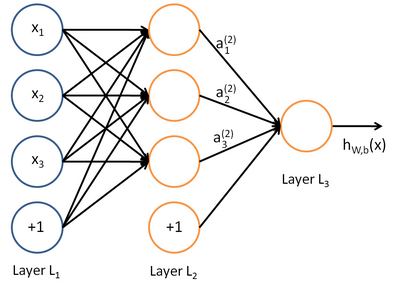
\includegraphics[width=0.5\textwidth]{Perceptron1.png}
	\caption{神经网络}
	\label{fig:Per0}
\end{figure}

图\ref{fig:Per0}中每个圆圈都是一个神经元,每条线表示神经元之间的连接。我们可以看到,上面的神经元被分成了多层,层与层之间的神经元有连接,而层内之间的神经元没有连接。最左边的层叫做\textbf{输入层},这层负责接收输入数据;最右边的层叫\textbf{输出层},我们可以从这层获取神经网络输出数据。输入层和输出层之间的层叫做\textbf{隐藏层}。

隐藏层比较多(大于2)的神经网络叫做深度神经网络。而深度学习,就是使用深层架构(比如,深度神经网络)的机器学习方法。

那么深层网络和浅层网络相比有什么优势呢?简单来说深层网络能够表达力更强。事实上,一个仅有一个隐藏层的神经网络就能拟合任何一个函数,但是它需要很多很多的神经元。而深层网络用少得多的神经元就能拟合同样的函数。也就是为了拟合一个函数,要么使用一个浅而宽的网络,要么使用一个深而窄的网络。而后者往往更节约资源。

深层网络也有劣势,就是它不太容易训练。简单的说,你需要大量的数据,很多的技巧才能训练好一个深层网络。这是个手艺活。


\section{感知器}\label{Per:2}
看到这里,如果你还是一头雾水,那也是很正常的。为了理解神经网络,我们应该先理解神经网络的组成单元------\textbf{神经元}。神经元也叫做\textbf{感知器}。感知器算法在上个世纪50-70年代很流行,也成功解决了很多问题。并且,感知器算法也是非常简单的。

\subsection{感知器的定义}\label{Per:3}

下图是一个感知器:

\begin{figure}[htbp]
	\centering
	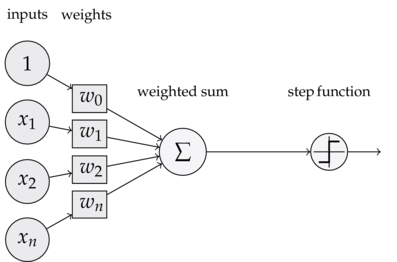
\includegraphics[width=0.5\textwidth]{Perceptron2.png}
	\caption{感知器}
\end{figure}

可以看到,一个感知器有如下组成部分:

\begin{itemize}
	\item
	      \textbf{输入权值}
	      一个感知器可以接收多个输入$(x_1, x_2,...,x_n\mid x_i\in\Re)$,每个输入上有一个\textbf{权值}$w_i\in\Re$,此外还有一个\textbf{偏置项}$b\in\Re$,就是上图中$w_0$。
	\item
	      \textbf{激活函数}
	      感知器的激活函数可以有很多选择,比如我们可以选择下面这个\textbf{阶跃函数}$f$来作为激活函数:
	      \begin{equation*}
		      f(x)=\left\{
		      \begin{aligned}
			      1 & \quad z>0       \\
			      0 & \quad otherwise
		      \end{aligned}
		      \right.
	      \end{equation*}
	\item
	      \textbf{输出} 感知器的输出由下面这个公式来计算
	      \begin{equation}
		      \label{eq:Per1}
		      y=f(w \bullet x + b)
	      \end{equation}
\end{itemize}

如果看完上面的公式一下子就晕了,不要紧,我们用一个简单的例子来帮助理解。

\begin{example}
	用感知器实现 \textcolor{main}{\textbf{and}} 函数
\end{example}

我们设计一个感知器,让它来实现 \textcolor{main}{\textbf{and}} 运算。程序员都知道,\textcolor{main}{\textbf{and}} 是一个二元函数(带有两个参数$x_1$和$x_2$),下面是它的\textbf{真值表}:


\begin{table}[htbp]
	\centering
	\setlength{\tabcolsep}{10mm}
	\caption{\textcolor{main}{\textbf{and}}真值表}
	\begin{tabular}{ccc}
		\hline
		$x_1$ & $x_2$ & $y$ \\ \hline
		0     & 0     & 0   \\
		0     & 1     & 0   \\
		1     & 0     & 0   \\
		1     & 1     & 1   \\ \hline
	\end{tabular}
	\label{tab:Per1}
\end{table}

为了计算方便,我们用0表示\textbf{false},用1表示\textbf{true}。这没什么难理解的,对于C语言程序员来说,这是天经地义的。

我们令$w_1=0.5;w_2=0.5;b=-0.8$,而激活函数$f$就是前面写出来的\textbf{阶跃函数},这时,感知器就相当于\textcolor{main}{\textbf{and}} 函数。不明白?我们验算一下:

输入上面真值表的第一行,即$x_1=0;x_2=0$,那么根据公式\ref{eq:Per1},计算输出:
\begin{align*}
	y & =f(w \bullet x + b) = f(w_1x_1+w_2x_2+b)    \\
	  & =f(0.5\times0+0.5\times0-0.8) = f(-0.8) = 0
\end{align*}
也就是当$x_1, x_2$都为0的时候,$y$为0,这就是表\ref{tab:Per1}的第一行。读者可以自行验证上述真值表的第二、三、四行。

\begin{example}
	用感知器实现 \textcolor{main}{\textbf{or}} 函数
\end{example}

同样,我们也可以用感知器来实现\textcolor{main}{\textbf{or}}运算。仅仅需要把偏置项$b$的值设置为$-0.3$就可以了。我们验算一下,下面是\textcolor{main}{\textbf{or}}运算的\textbf{真值表}:


\begin{table}[htbp]
	\centering
	\setlength{\tabcolsep}{10mm}
	\caption{\textcolor{main}{\textbf{or}}真值表}
	\begin{tabular}{ccc}
		\hline
		$x_1$ & $x_2$ & $y$ \\ \hline
		0     & 0     & 0   \\
		0     & 1     & 1   \\
		1     & 0     & 1   \\
		1     & 1     & 1   \\ \hline
	\end{tabular}
	\label{tab:Per2}
\end{table}


我们来验算第二行,这时的输入是$x_1=0;x_2=1$,带入公式\ref{eq:Per1}:
\begin{align*}
	y & =f(w \bullet x + b) = f(w_1x_1+w_2x_2+b)   \\
	  & =f(0.5\times1+0.5\times0-0.3) = f(0.2) = 1
\end{align*}
也就是当$x_1=0;x_2=1$时,$y$为1,即表\ref{tab:Per2}第二行。读者可以自行验证其它行。


\subsection{感知器还能做什么}\label{Per:4}

事实上,感知器不仅仅能实现简单的布尔运算。它可以拟合任何的线性函数,任何\textbf{线性分类}或\textbf{线性回归}问题都可以用感知器来解决。前面的布尔运算可以看作是\textbf{二分类}问题,即给定一个输入,输出0(属于分类0)或1(属于分类1)。如图\ref{fig:Per1_a}所示,\textcolor{main}{\textbf{and}}运算是一个线性分类问题,即可以用一条直线把分类0(false,红叉表示)和分类1(true,绿点表示)分开。
然而,感知器却不能实现异或运算,如图\ref{fig:Per1_b}所示,异或运算不是线性的,你无法用一条直线把分类0和分类1分开。

\begin{figure}[htbp]
	\centering
	\subfigure[]{
		\begin{minipage}[t]{0.5\linewidth}
			\centering
			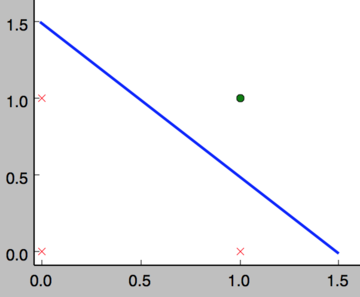
\includegraphics[width=2in]{Perceptron3.png}
			\label{fig:Per1_a}
			%\caption{fig1}
		\end{minipage}%
	}%
	\subfigure[]{
		\begin{minipage}[t]{0.5\linewidth}
			\centering
			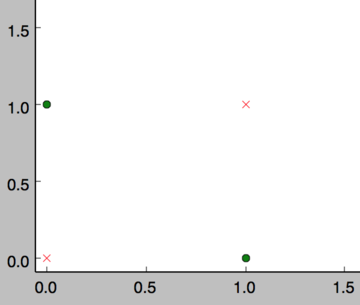
\includegraphics[width=2in]{Perceptron4.png}
			\label{fig:Per1_b}
			%\caption{fig2}
		\end{minipage}%
	}%
	\centering
	\caption{真值图}
	\label{fig:Per1}
\end{figure}


\subsection{感知器的训练}\label{Per:4}

现在,你可能困惑前面的权重项和偏置项的值是如何获得的呢?这就要用到感知器训练算法:将权重项和偏置项初始化为0,然后,利用下面的\textbf{感知器规则}迭代的修改$w_i$和$b$,直到训练完成。
\begin{align*}
	w_i & \gets w_i+\Delta w_i \\
	b   & \gets b+\Delta b
\end{align*}
其中:
\begin{align*}
	\Delta w_i & =\eta(t-y)x_i \\
	\Delta b   & =\eta(t-y)
\end{align*}

$w_i$是与输入$x_i$对应的权重项,$b$是偏置项。事实上,可以把$b$看作是值永远为1的输入$x_b$所对应的权重。$t$是训练样本的\textbf{实际值},一般称之为\textbf{label}。而$y$是感知器的输出值,它是根据公式\ref{eq:Per1}计算得出。$\eta$是一个称为\textbf{学习速率}的常数,其作用是控制每一步调整权的幅度。

每次从训练数据中取出一个样本的输入向量$x$,使用感知器计算其输出$y$,再根据上面的规则来调整权重。每处理一个样本就调整一次权重。经过多轮迭代后(即全部的训练数据被反复处理多轮),就可以训练出感知器的权重,使之实现目标函数。


\section{编程实战:实现感知器}\label{Per:5}

\begin{note}
	完整代码请参考GitHub: \url{https://github.com/hanbt/learn_dl/blob/master/perceptron.py}
	(python2.7)
\end{note}


对于程序员来说,没有什么比亲自动手实现学得更快了,而且,很多时候一行代码抵得上千言万语。接下来我们就将实现一个感知器。

下面是一些说明:
\begin{itemize}
	\item
	      使用python语言。python在机器学习领域用的很广泛,而且,写python程序真的很轻松。
	\item
	      面向对象编程。面向对象是特别好的管理复杂度的工具,应对复杂问题时,用面向对象设计方法很容易将复杂问题拆解为多个简单问题,从而解救我们的大脑。
	\item
	      没有使用numpy。numpy实现了很多基础算法,对于实现机器学习算法来说是个必备的工具。但为了降低读者理解的难度,下面的代码只用到了基本的python(省去您去学习numpy的时间)。
\end{itemize}


下面是感知器类的实现,非常简单。去掉注释只有27行,而且还包括为了美观(每行不超过60个字符)而增加的很多换行。
\begin{lstlisting}
class Perceptron(object):
    def __init__(self, input_num, activator):
        '''
        初始化感知器,设置输入参数的个数,以及激活函数。
        激活函数的类型为double -> double
        '''
        self.activator = activator
        # 权重向量初始化为0
        self.weights = [0.0 for _ in range(input_num)]
        # 偏置项初始化为0
        self.bias = 0.0
    def __str__(self):
        '''
        打印学习到的权重、偏置项
        '''
        return 'weights\t:%s\nbias\t:%f\n' % (self.weights, self.bias)
    def predict(self, input_vec):
        '''
        输入向量,输出感知器的计算结果
        '''
        # 把input_vec[x1,x2,x3...]和weights[w1,w2,w3,...]打包在一起
        # 变成[(x1,w1),(x2,w2),(x3,w3),...]
        # 然后利用map函数计算[x1*w1, x2*w2, x3*w3]
        # 最后利用reduce求和
        return self.activator(
            reduce(lambda a, b: a + b,
                   map(lambda (x, w): x * w,  
                       zip(input_vec, self.weights))
                , 0.0) + self.bias)
    def train(self, input_vecs, labels, iteration, rate):
        '''
        输入训练数据:一组向量、与每个向量对应的label;以及训练轮数、学习率
        '''
        for i in range(iteration):
            self._one_iteration(input_vecs, labels, rate)
    def _one_iteration(self, input_vecs, labels, rate):
        '''
        一次迭代,把所有的训练数据过一遍
        '''
        # 把输入和输出打包在一起,成为样本的列表[(input_vec, label), ...]
        # 而每个训练样本是(input_vec, label)
        samples = zip(input_vecs, labels)
        # 对每个样本,按照感知器规则更新权重
        for (input_vec, label) in samples:
            # 计算感知器在当前权重下的输出
            output = self.predict(input_vec)
            # 更新权重
            self._update_weights(input_vec, output, label, rate)
    def _update_weights(self, input_vec, output, label, rate):
        '''
        按照感知器规则更新权重
        '''
        # 把input_vec[x1,x2,x3,...]和weights[w1,w2,w3,...]打包在一起
        # 变成[(x1,w1),(x2,w2),(x3,w3),...]
        # 然后利用感知器规则更新权重
        delta = label - output
        self.weights = map(
            lambda (x, w): w + rate * delta * x,
            zip(input_vec, self.weights))
        # 更新bias
        self.bias += rate * delta
\end{lstlisting}


接下来,我们利用这个感知器类去实现\textcolor{main}{\textbf{and}}函数。
\begin{lstlisting}
def f(x):
    '''
    定义激活函数f
    '''
    return 1 if x > 0 else 0
def get_training_dataset():
    '''
    基于and真值表构建训练数据
    '''
    # 构建训练数据
    # 输入向量列表
    input_vecs = [[1,1], [0,0], [1,0], [0,1]]
    # 期望的输出列表,注意要与输入一一对应
    # [1,1] -> 1, [0,0] -> 0, [1,0] -> 0, [0,1] -> 0
    labels = [1, 0, 0, 0]
    return input_vecs, labels    
def train_and_perceptron():
    '''
    使用and真值表训练感知器
    '''
    # 创建感知器,输入参数个数为2(因为and是二元函数),激活函数为f
    p = Perceptron(2, f)
    # 训练,迭代10轮, 学习速率为0.1
    input_vecs, labels = get_training_dataset()
    p.train(input_vecs, labels, 10, 0.1)
    #返回训练好的感知器
    return p
if __name__ == '__main__': 
    # 训练and感知器
    and_perception = train_and_perceptron()
    # 打印训练获得的权重
    print and_perception
    # 测试
    print '1 and 1 = %d' % and_perception.predict([1, 1])
    print '0 and 0 = %d' % and_perception.predict([0, 0])
    print '1 and 0 = %d' % and_perception.predict([1, 0])
    print '0 and 1 = %d' % and_perception.predict([0, 1])
\end{lstlisting}

将上述程序保存为perceptron.py文件,通过命令行执行这个程序,其运行结果为:

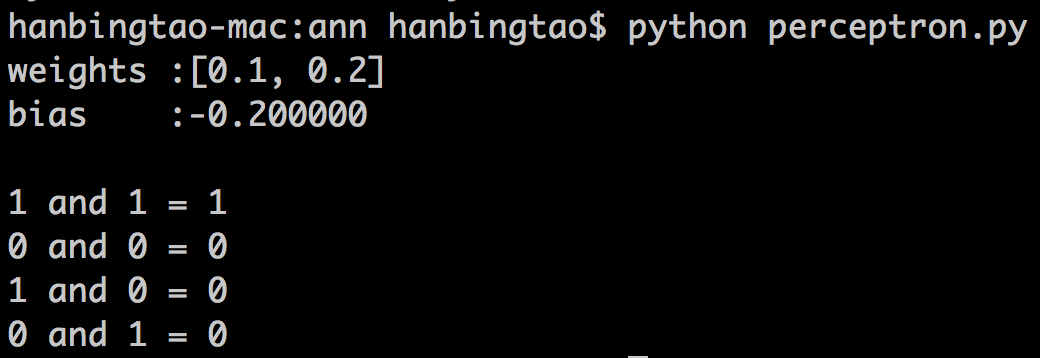
\includegraphics[width=0.8\textwidth]{Perceptron5.png}

神奇吧!感知器竟然完全实现了\textcolor{main}{\textbf{and}}函数。读者可以尝试一下利用感知器实现其它函数。

\section{小结}

终于看(写)到小结了...,大家都累了。对于零基础的你来说,走到这里应该已经很烧脑了吧。没关系,休息一下。值得高兴的是,你终于已经走出了深度学习入门的第一步,这是巨大的进步;坏消息是,这仅仅是最简单的部分,后面还有无数艰难险阻等着你。不过,你学的困难往往意味着别人学的也困难,掌握一门高门槛的技艺,进可糊口退可装逼,是很值得的。

下一篇文章,我们将讨论另外一种感知器:\textbf{线性单元},并由此引出一种可能是最最重要的优化算法:\textbf{梯度下降}算法。
\chapter{线性单元和梯度下降}\label{chap:Line}

\begin{introduction}
	\item 线性单元是啥~\ref{Line:1}
	\item 线性单元的模型~\ref{Line:2}
	\item 监督学习和无监督学习~\ref{Line:3}
	\item 线性单元的目标函数~\ref{Line:4}
	\item 梯度下降优化算法~\ref{Line:5}
	\item $\nabla{E}({w})$的推导~\ref{Line:6}
	\item 随机梯度下降算法~\ref{Line:7}
	\item 编程实战:实现线性单元~\ref{Line:8}
\end{introduction}


在上一篇文章中,我们已经学会了编写一个简单的感知器,并用它来实现一个线性分类器。你应该还记得用来训练感知器的『感知器规则』。然而,我们并没有关心这个规则是怎么得到的。本文通过介绍另外一种『感知器』,也就是『线性单元』,来说明关于机器学习一些基本的概念,比如模型、目标函数、优化算法等等。这些概念对于所有的机器学习算法来说都是通用的,掌握了这些概念,就掌握了机器学习的基本套路。

\section{线性单元是啥}\label{Line:1}
感知器有一个问题,当面对的数据集不是\textbf{线性可分}的时候,『感知器规则』可能无法收敛,这意味着我们永远也无法完成一个感知器的训练。为了解决这个问题,我们使用一个\textbf{可导}的\textbf{线性函数}来替代感知器的\textbf{阶跃函数},这种感知器就叫做\textbf{线性单元}。线性单元在面对线性不可分的数据集时,会收敛到一个最佳的近似上。

为了简单起见,我们可以设置线性单元的激活函数$f$为$f(x)=x$, 这样的线性单元如图\ref{fig:Line1}所示,对比此前我们讲过的感知器如图\ref{fig:Line2}所示

\begin{figure}[h]
	\centering
	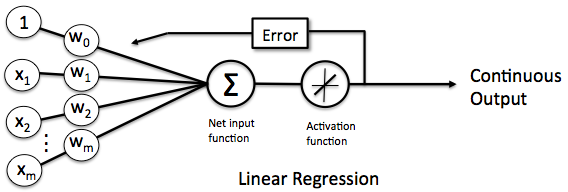
\includegraphics[width=0.7\textwidth]{Line1.png}
	\caption{线性单元}
	\label{fig:Line1}
\end{figure}

\begin{figure}[h]
	\centering
	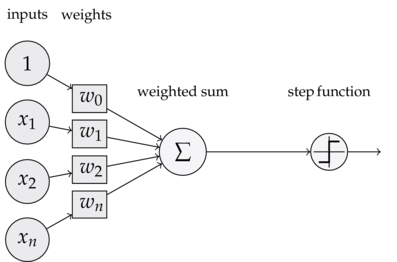
\includegraphics[width=0.5\textwidth]{Line2.png}
	\caption{感知器}
	\label{fig:Line2}
\end{figure}

这样替换了激活函数$f$之后,\textbf{线性单元}将返回一个\textbf{实数值}而不是\textbf{0, 1分类}。因此线性单元用来解决\textbf{回归}问题而不是\textbf{分类}问题。

\subsection{线性单元的模型}\label{Line:2}

当我们说\textbf{模型}时,我们实际上在谈论根据输入$x$预测输出$y$的\textbf{算法}。比如,$x$可以是一个人的工作年限,$y$可以是他的月薪,我们可以用某种算法来根据一个人的工作年限来预测他的收入。比如:
\[y=h(x)=w*x+b\]

函数$h(x)$叫做\textbf{假设},而$w$、$b$是它的\textbf{参数}。我们假设参数$w=1000$,参数$b=500$,如果一个人的工作年限是5年的话,我们的模型会预测他的月薪为
\[y=h(x)=1000*5+500=5500(\mbox{元})\]

你也许会说,这个模型太不靠谱了。是这样的,因为我们考虑的因素太少了,仅仅包含了工作年限。如果考虑更多的因素,比如所处的行业、公司、职级等等,可能预测就会靠谱的多。我们把工作年限、行业、公司、职级这些信息,称之为\textbf{特征}。对于一个工作了5年,在IT行业,百度工作,职级T6这样的人,我们可以用这样的一个特征向量来表示他
\[
	x = (\emph{5, IT, 百度, T6})
\]


既然输入$x$变成了一个具备四个特征的向量,相对应的,仅仅一个参数$w$就不够用了,我们应该使用4个参数\(w_1,w_2,w_3,w_4\),每个特征对应一个。这样,我们的模型就变成
\[y=h(x)=w_1*x_1+w_2*x_2+w_3*x_3+w_4*x_4+b\]

其中,\(x_1\)对应工作年限,\(x_2\)对应行业,\(x_3\)对应公司,\(x_4\)对应职级。

为了书写和计算方便,我们可以令\(w_0\)等于\(b\),同时令\(w_0\)对应于特征\(x_0\)。由于\(x_0\)其实并不存在,我们可以令它的值永远为1。也就是说
\[
	b = w_0 * x_0\qquad \mbox{其中} x_0=1
\]

这样上面的式子就可以写成
\begin{align*}
	y=h(x) & =w_1*x_1+w_2*x_2+w_3*x_3+w_4*x_4+b       \\
	       & =w_0*x_0+w_1*x_1+w_2*x_2+w_3*x_3+w_4*x_4
\end{align*}


我们还可以把上式写成向量的形式
\begin{equation}
	\label{eq:Line1}
	y=h(x)=w^Tx
\end{equation}



长成这种样子模型就叫做\textbf{线性模型},因为输出\(y\)就是输入特征\(x_1,x_2,x_3,...\)的\textbf{线性组合}。



\subsection{监督学习和无监督学习}\label{Line:3}

接下来,我们需要关心的是这个模型如何训练,也就是参数\(w\)取什么值最合适。

机器学习有一类学习方法叫做\textbf{监督学习},它是说为了训练一个模型,我们要提供这样一堆训练样本:每个训练样本既包括输入特征\(x\),也包括对应的输出\(y\)(\(y\)也叫做\textbf{标记,label})。也就是说,我们要找到很多人,我们既知道他们的特征(工作年限,行业...),也知道他们的收入。我们用这样的样本去训练模型,让模型既看到我们提出的每个问题(输入特征\(x\)),也看到对应问题的答案(标记\(y\))。当模型看到足够多的样本之后,它就能总结出其中的一些规律。然后,就可以预测那些它没看过的输入所对应的答案了。

另外一类学习方法叫做\textbf{无监督学习},这种方法的训练样本中只有\(x\)而没有\(y\)。模型可以总结出特征\(x\)的一些规律,但是无法知道其对应的答案\(y\)。

很多时候,既有\(x\)又有\(y\)的训练样本是很少的,大部分样本都只有\(x\)。比如在语音到文本(STT)的识别任务中,\(x\)是语音,\(y\)是这段语音对应的文本。我们很容易获取大量的语音录音,然而把语音一段一段切分好并\textbf{标注}上对应文字则是非常费力气的事情。这种情况下,为了弥补带标注样本的不足,我们可以用\textbf{无监督学习方法}先做一些\textbf{聚类},让模型总结出哪些音节是相似的,然后再用少量的带标注的训练样本,告诉模型其中一些音节对应的文字。这样模型就可以把相似的音节都对应到相应文字上,完成模型的训练。

\subsection{线性单元的目标函数}\label{Line:4}

现在,让我们只考虑\textbf{监督学习}。

在监督学习下,对于一个样本,我们知道它的特征\(x\),以及标记\(y\)。同时,我们还可以根据模型\(h(x)\)计算得到输出\(\bar{y}\)。注意这里面我们用\(y\)表示训练样本里面的\textbf{标记},也就是\textbf{实际值};用带上划线的\(\bar{y}\)表示模型计算的出来的\textbf{预测值}。我们当然希望模型计算出来的\(\bar{y}\)和\(y\)越接近越好。

数学上有很多方法来表示的\(\bar{y}\)和\(y\)的接近程度,比如我们可以用\(\bar{y}\)和\(y\)的差的平方的\(\frac{1}{2}\)来表示它们的接近程度
\[
	e=\frac{1}{2}(y-\bar{y})^2
\]

我们把\(e\)叫做\textbf{单个样本}的\textbf{误差}。至于为什么前面要乘\(\frac{1}{2}\),是为了后面计算方便。

训练数据中会有很多样本,比如\(N\)个,我们可以用训练数据中\textbf{所有样本}的误差的\textbf{和},来表示模型的误差\(E\),也就是
\[
	E=e^{(1)}+e^{(2)}+e^{(3)}+...+e^{(n)}
\]

上式的\(e^{(1)}\)表示第一个样本的误差,\(e^{(2)}\)表示第二个样本的误差......。

我们还可以把上面的式子写成和式的形式。使用和式,不光书写起来简单,逼格也跟着暴涨,一举两得。所以一定要写成下面这样

\begin{equation}
	\label{eq:Line2}
	E = e^{(1)}+e^{(2)}+e^{(3)}+...+e^{(n)}=\sum_{i=1}^{n}e^{(i)} =\frac{1}{2}\sum_{i=1}^{n}(y^{(i)}-\bar{y}^{(i)})^2
\end{equation}


其中
\begin{align*}
	\bar{y}^{(i)} =h(x^{(i)}) = w^T{x^{(i)}}
\end{align*}

公式\ref{eq:Line2}中,\(x^{(i)}\)表示第\(i\)个训练样本的\textbf{特征},\(y^{(i)}\)表示第\(i\)个样本的\textbf{标记},我们也可以用\textbf{元组}\((x^{(i)},y^{(i)})\)表示第\(i\)\textbf{训练样本}。\(\bar{y}^{(i)}\)则是模型对第\(i\)个样本的\textbf{预测值}。


我们当然希望对于一个训练数据集来说,误差最小越好,也就是公式\ref{eq:Line2}的值越小越好。对于特定的训练数据集来说,\((x^{(i)},y^{(i)})\)的值都是已知的,所以公式\ref{eq:Line2}其实是参数\({w}\)的函数。
\begin{align*}
	E({w}) =\frac{1}{2}\sum_{i=1}^{n}(y^{(i)}-\bar{y}^{(i)})^2 =\frac{1}{2}\sum_{i=1}^{n}({y^{(i)}-{w}^Tx^{(i)}})^2
\end{align*}


由此可见,模型的训练,实际上就是求取到合适的\({w}\),使(式2)取得最小值。这在数学上称作\textbf{优化问题},而\(E({w})\)就是我们优化的目标,称之为\textbf{目标函数}。


\subsection{梯度下降优化算法}\label{Line:5}

大学时我们学过怎样求函数的极值。函数\(y=f(x)\)的极值点,就是它的导数\(f'(x)=0\)的那个点。因此我们可以通过解方程\(f'(x)=0\),求得函数的极值点\((x_0,y_0)\)。

不过对于计算机来说,它可不会解方程。但是它可以凭借强大的计算能力,一步一步的去把函数的极值点『试』出来。如图\ref{fig:Line3}所示:


\begin{figure}[htbp]
	\centering
	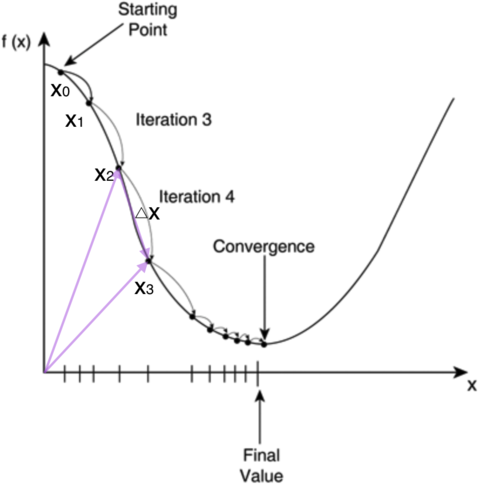
\includegraphics[width=0.6\textwidth]{Line3.png}
	\caption{极值点搜索图}
	\label{fig:Line3}
\end{figure}

首先,我们随便选择一个点开始,比如上图的\(x_0\)点。接下来,每次迭代修改\(x\)的为\(x_1,x_2,x_3,...\),经过数次迭代后最终达到函数最小值点。

你可能要问了,为啥每次修改\(x\)的值,都能往函数最小值那个方向前进呢?这里的奥秘在于,我们每次都是向函数\(y=f(x)\)的\textbf{梯度}的\textbf{相反方向}来修改\(x\)。什么是\textbf{梯度}呢?翻开大学高数课的课本,我们会发现\textbf{梯度}是一个向量,它指向\textbf{函数值上升最快}的方向。显然,梯度的反方向当然就是函数值下降最快的方向了。我们每次沿着梯度相反方向去修改\(x\)的
值,当然就能走到函数的最小值附近。之所以是最小值附近而不是最小值那个点,是因为我们每次移动的步长不会那么恰到好处,有可能最后一次迭代走远了越过了
最小值那个点。步长的选择是门手艺,如果选择小了,那么就会迭代很多轮才能走到最小值附近;如果选择大了,那可能就会越过最小值很远,收敛不到一个好的点
上。

按照上面的讨论,我们就可以写出梯度下降算法的公式
\[
	{x}_{new}={x}_{old}-\eta\nabla{f(x)}
\]
其中,\(\nabla\)是\textbf{梯度算子},\(\nabla{f(x)}\)就是指{}\(f(x)\)的梯度。\(\eta\)是步长,也称作\textbf{学习速率}。

对于上一节列出的目标函数(公式\ref{eq:Line2})
\[
	E({w})=\frac{1}{2}\sum_{i=1}^{n}({y^{(i)}-\bar{y}^{(i)}})^2
\]

梯度下降算法可以写成
\[
	{w}_{new}={w}_{old}-\eta\nabla{E({w})}
\]
聪明的你应该能想到,如果要求目标函数的\textbf{最大值},那么我们就应该用\textbf{梯度上升}算法,它的参数修改规则是
\[
	{w}_{new}={w}_{old}+\eta\nabla{E({w})}
\]

下面,请先做几次深呼吸,让你的大脑补充足够的新鲜的氧气,我们要来求取\(\nabla{E}({w})\),然后带入上式,就能得到线性单元的参数修改规则。

关于\(\nabla{E({w})}\)的推导过程,我单独把它们放到一节中。您既可以选择慢慢看,也可以选择无视。在这里,您只需要知道,经过一大串推导,目标函数\(E(w)\)的梯度是
\[
	\nabla{E({w})}=-\sum_{i=1}^{n}(y^{(i)}-\bar{y}^{(i)}){x}^{(i)}
\]

因此,线性单元的参数修改规则最后是这个样子
\begin{equation}
	{w}_{new}={w}_{old}+\eta\sum_{i=1}^{n}(y^{(i)}-\bar{y}^{(i)}){x}^{(i)}
	\label{eq:Line3}
\end{equation}


有了上面这个式子,我们就可以根据它来写出训练线性单元的代码了。

需要说明的是,如果每个样本有M个特征,则上式中的\({x},{w}\)都是M+1维\textbf{向量}(因为我们加上了一个恒为1的虚拟特征\(x_0\),参考前面的内容),而\(y\)是\textbf{标量}。用高逼格的数学符号表示,就是
\[
	{x},{w}\in\Re^{(M+1)},
	y\in\Re^1
\]

为了让您看明白说的是啥,我吐血写下下面这个解释(写这种公式可累可累了)。因为{}\({w},{x}\)是M+1维\textbf{列向量},所以(公式\ref{eq:Line3})可以写成
\begin{equation*}
	\begin{bmatrix}
		w_0 \\
		w_1 \\
		w_2 \\
		... \\
		w_m \\
	\end{bmatrix}_{new}=
	\begin{bmatrix}
		w_0 \\
		w_1 \\
		w_2 \\
		... \\
		w_m \\
	\end{bmatrix}_{old}+\eta\sum_{i=1}^{n}(y^{(i)}-\bar{y}^{(i)})
	\begin{bmatrix}
		1         \\
		x_1^{(i)} \\
		x_2^{(i)} \\
		...       \\
		x_m^{(i)} \\
	\end{bmatrix}
\end{equation*}
如果您还是没看明白,建议您也吐血再看一下大学时学过的《线性代数》吧。

\subsection{$\nabla{E}({w})$的推导}\label{Line:6}

这一节你尽可以跳过它,并不太会影响到全文的理解。当然如果你非要弄明白每个细节,那恭喜你骚年,机器学习的未来一定是属于你的。

首先,我们先做一个简单的前戏。我们知道函数的梯度的定义就是它相对于各个变量的\textbf{偏导数},所以我们写下下面的式子
\begin{align*}
	\nabla{E({w})} =\frac{\partial}{\partial{w}}E({w}) =\frac{\partial}{\partial{w}}\frac{1}{2}\sum_{i=1}^{n}(y^{(i)}-\bar{y}^{(i)})^2
\end{align*}
可接下来怎么办呢?我们知道和的导数等于导数的和,所以我们可以先把求和符号\(\sum\)里面的导数求出来,然后再把它们加在一起就行了,也就是
\begin{align*}
	\frac{\partial}{\partial{w}}\frac{1}{2}\sum_{i=1}^{n}(y^{(i)}-\bar{y}^{(i)})^2 = \frac{1}{2}\sum_{i=1}^{n}\frac{\partial}{\partial{w}}(y^{(i)}-\bar{y}^{(i)})^2
\end{align*}
现在我们可以不管高大上的\(\sum\)了,先专心把里面的导数求出来。
\begin{align*}
	\frac{\partial}{\partial{w}}(y^{(i)}-\bar{y}^{(i)})^2 = \frac{\partial}{\partial{w}}(y^{(i)2}-2\bar{y}^{(i)}y^{(i)}+\bar{y}^{(i)2})
\end{align*}
我们知道,\(y\)是与\({w}\)无关的常数,而\(\bar{y}={w}^T{x}\),下面我们根据链式求导法则来求导(上大学时好像叫复合函数求导法则)
\[
	\frac{\partial{E({w})}}{\partial{w}}=\frac{\partial{E(\bar{y})}}{\partial\bar{y}}\frac{\partial{\bar{y}}}{\partial{w}}
\]

我们分别计算上式等号右边的两个偏导数
\begin{align*}
	\frac{\partial{E({w})}}{\partial\bar{y}}=
	 & \frac{\partial}{\partial\bar{y}}(y^{(i)2}-2\bar{y}^{(i)}y^{(i)}+\bar{y}^{(i)2}) = -2y^{(i)}+2\bar{y}^{(i)} \\
	\frac{\partial{\bar{y}}}{\partial{w}}=
	 & \frac{\partial}{\partial{w}}{w}^T{x}= {x}
\end{align*}


代入,我们求得\(\sum\)里面的偏导数是
\begin{align*}
	\frac{\partial}{\partial{w}}(y^{(i)}-\bar{y}^{(i)})^2 = 2(-y^{(i)}+\bar{y}^{(i)}){x}
\end{align*}


最后代入\(\nabla{E}({w})\),求得
\begin{align*}
	\nabla{E({w})} =\frac{1}{2}\sum_{i=1}^{n}\frac{\partial}{\partial{w}}(y^{(i)}-\bar{y}^{(i)})^2 =\frac{1}{2}\sum_{i=1}^{n}2(-y^{(i)}+\bar{y}^{(i)}){x} =-\sum_{i=1}^{n}(y^{(i)}-\bar{y}^{(i)}){x}
\end{align*}


至此,大功告成。

\subsection{随机梯度下降算法}\label{Line:7}

如果我们根据(公式\ref{eq:Line3})来训练模型,那么我们每次更新\({w}\)的迭代,要遍历训练数据中所有的样本进行计算,我们称这种算法叫做\textbf{批梯度下降(Batch Gradient Descent)}。如果我们的样本非常大,比如数百万到数亿,那么计算量异常巨大。因此,实用的算法是SGD算法。在SGD算法中,每次更新\({w}\)的迭代,只计算一个样本。这样对于一个具有数百万样本的训练数据,完成一次遍历就会对\({w}\)更新数百万次,效率大大提升。由于样本的噪音和随机性,每次更新\({w}\)并不一定按照减少\(E\)的方向。然而,虽然存在一定随机性,大量的更新总体上沿着减少\(E\)的方向前进的,因此最后也能收敛到最小值附近。下图展示了SGD和BGD的区别

\begin{figure}[htbp]
	\centering
	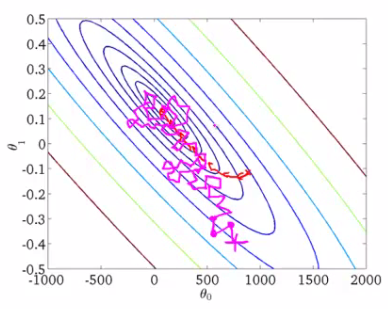
\includegraphics[width=0.7\textwidth]{Line4.png}
	\caption{极值点搜索图}
	\label{fig:Line4}
\end{figure}

如图\ref{fig:Line4},椭圆表示的是函数值的等高线,椭圆中心是函数的最小值点。红色是BGD的逼近曲线,而紫色是SGD的逼近曲线。我们可以看到BGD是一直向着最低点前进的,而SGD明显躁动了许多,但总体上仍然是向最低点逼近的。

最后需要说明的是,SGD不仅仅效率高,而且随机性有时候反而是好事。今天的目标函数是一个『凸函数』,沿着梯度反方向就能找到全局唯一的最小值。然而对于非凸函数来说,存在许多局部最小值。随机性有助于我们逃离某些很糟糕的局部最小值,从而获得一个更好的模型。


\section{编程实战:实现线性单元}\label{Line:8}

\begin{note}
	完整代码请参考GitHub: \url{https://github.com/hanbt/learn_dl/blob/master/linear_unit.py}
	(python2.7)
\end{note}

接下来,让我们撸一把代码。

因为我们已经写了感知器的代码,因此我们先比较一下感知器模型和线性单元模型,看看哪些代码能够复用。

\begin{table}[htbp]
	\centering
	\setlength{\tabcolsep}{7mm}
	\caption{模型函数对比}
	\begin{tabular}{ccc}
		\hline
		算法                                   & 感知器                             & 线性单元                           \\ \hline
		\multirow{2}{*}{\centering 模型$h(x)$} & $y=f(w^Tx)$                        & $y=f(w^Tx)$                        \\
		                                       & f(x) = 1*(z>0)                     & $f(z)=z$                           \\
		训练规则                               & \({w}\gets{w}+\eta(y-\bar{y}){x}\) & \({w}\gets{w}+\eta(y-\bar{y}){x}\) \\ \hline
	\end{tabular}
\end{table}

比较的结果令人震惊,原来除了激活函数\(f\)不同之外,两者的模型和训练规则是一样的(在上表中,线性单元的优化算法是SGD算法)。那么,我们只需要把感知器的激活函数进行替换即可。感知器的代码请参考第\ref{chap:Per}章,这里就不再重复了。对于一个养成良好习惯的程序员来说,重复代码是不可忍受的。大家应该把代码保存在一个代码库中(比如git)。
\begin{lstlisting}
from perceptron import Perceptron
#定义激活函数f
f = lambda x: x
class LinearUnit(Perceptron):
    def __init__(self, input_num):
        '''初始化线性单元,设置输入参数的个数'''
    Perceptron.__init__(self, input_num, f)
\end{lstlisting}

通过继承Perceptron,我们仅用几行代码就实现了线性单元。这再次证明了面向对象编程范式的强大。

接下来,我们用简单的数据进行一下测试。
\begin{lstlisting}
def get_training_dataset():
    '''
    捏造5个人的收入数据
    '''
    # 构建训练数据
    # 输入向量列表,每一项是工作年限
    input_vecs = [[5], [3], [8], [1.4], [10.1]]
    # 期望的输出列表,月薪,注意要与输入一一对应
    labels = [5500, 2300, 7600, 1800, 11400]
    return input_vecs, labels    
def train_linear_unit():
    '''
    使用数据训练线性单元
    '''
    # 创建感知器,输入参数的特征数为1(工作年限)
    lu = LinearUnit(1)
    # 训练,迭代10轮, 学习速率为0.01
    input_vecs, labels = get_training_dataset()
    lu.train(input_vecs, labels, 10, 0.01)
    #返回训练好的线性单元
    return lu
if __name__ == '__main__': 
    '''训练线性单元'''
    linear_unit = train_linear_unit()
    # 打印训练获得的权重
    print linear_unit
    # 测试
    print 'Work 3.4 years, monthly salary = %.2f' % linear_unit.predict([3.4])
    print 'Work 15 years, monthly salary = %.2f' % linear_unit.predict([15])
    print 'Work 1.5 years, monthly salary = %.2f' % linear_unit.predict([1.5])
    print 'Work 6.3 years, monthly salary = %.2f' % linear_unit.predict([6.3])
\end{lstlisting}

程序运行结果如下图:

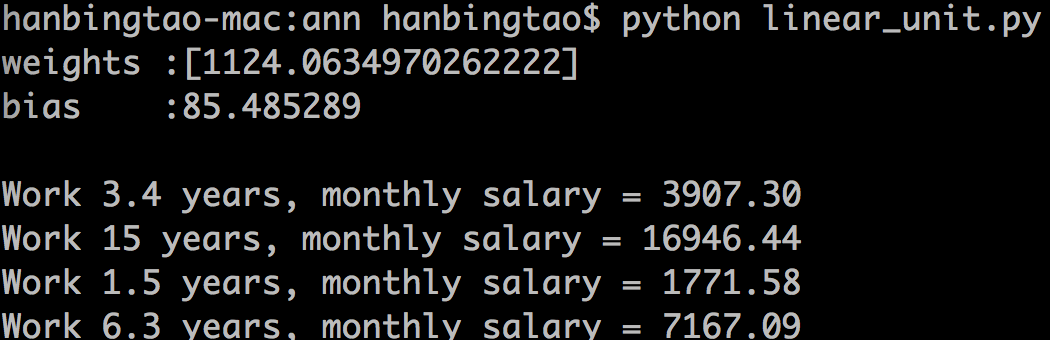
\includegraphics[width=0.7\textwidth]{Line5.png}


拟合的直线如下图:

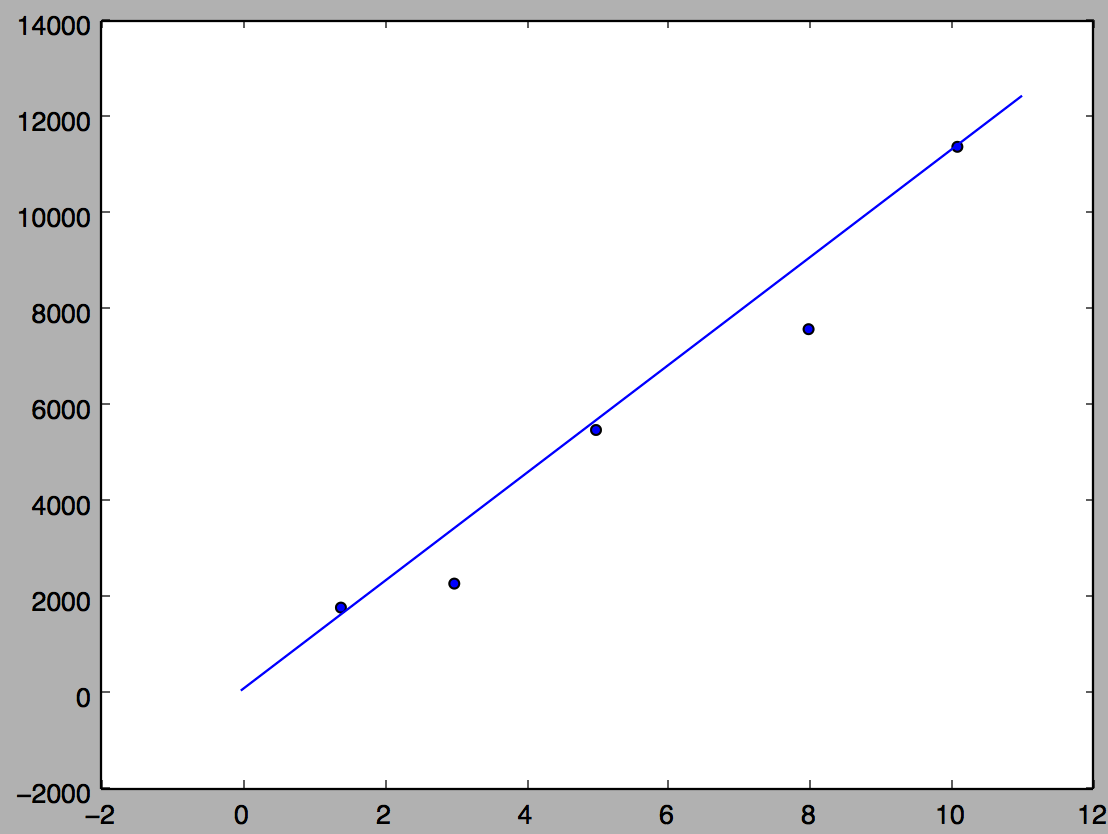
\includegraphics[width=0.7\textwidth]{Line6.png}


\section{小结}

事实上,一个机器学习算法其实只有两部分

\begin{itemize}
	\item
	      \emph{模型} 从输入特征\({x}\)预测输入\(y\)的那个函数\(h(x)\)
	\item
	      \emph{目标函数} 目标函数取最小(最大)值时所对应的参数值,就是模型的参数的\textbf{最优值}。很多时候我们只能获得目标函数的\textbf{局部最小(最大)值},因此也只能得到模型参数的\textbf{局部最优值}。
\end{itemize}

因此,如果你想最简洁的介绍一个算法,列出这两个函数就行了。

接下来,你会用\textbf{优化算法}去求取目标函数的最小(最大)值。\textbf{{[}随机{]}梯度\{下降\textbar 上升\}}算法就是一个\textbf{优化算法}。针对同一个\textbf{目标函数},不同的\textbf{优化算法}会推导出不同的\textbf{训练规则}。我们后面还会讲其它的优化算法。

其实在机器学习中,算法往往并不是关键,真正的关键之处在于选取特征。选取特征需要我们人类对问题的深刻理解,经验、以及思考。而\textbf{神经网络}算法的一个优势,就在于它能够自动学习到应该提取什么特征,从而使算法不再那么依赖人类,而这也是神经网络之所以吸引人的一个方面。

现在,经过漫长的烧脑,你已经具备了学习\textbf{神经网络}的必备知识。下一篇文章,我们将介绍本系列文章的主角:\textbf{神经网络},以及用来训练神经网络的大名鼎鼎的算法:\textbf{反向传播}算法。至于现在,我们应该暂时忘记一切,尽情奖励自己一下吧。




\chapter{神经网络和反向传播算法}\label{chap:Bp}

\begin{introduction}
	\item 神经元~\ref{Bp:1}
	\item 神经网络是啥~\ref{Bp:2}
	\item 计算神经网络的输出~\ref{Bp:3}
	\item 神经网络的矩阵表示~\ref{Bp:4}
	\item 神经网络的训练~\ref{Bp:5}
	\item 反向传播算法~\ref{Bp:6}
	\item 反向传播算法的推导~\ref{Bp:7}
	\item 编程实战:神经网络的实现~\ref{Bp:8},\ref{Bp:12}
	\item 神经网络实战:手写数字识别~\ref{Bp:9}
	\item 超参数的确定~\ref{Bp:10}
	\item 模型的训练和评估~\ref{Bp:11}
	\item 向量化编程~\ref{Bp:13}
\end{introduction}

在上一篇文章中,我们已经掌握了机器学习的基本套路,对模型、目标函数、优化算法这些概念有了一定程度的理解,而且已经会训练单个的感知器或者线性单元了。在这篇文章中,我们将把这些单独的单元按照一定的规则相互连接在一起形成\textbf{神经网络},从而奇迹般的获得了强大的学习能力。我们还将介绍这种网络的训练算法:\textbf{反向传播算法}。最后,我们依然用代码实现一个神经网络。如果您能坚持到本文的结尾,将会看到我们用自己实现的神经网络去识别手写数字。现在请做好准备,您即将双手触及到深度学习的大门。


\section{神经元}\label{Bp:1}

神经元和感知器本质上是一样的,只不过我们说感知器的时候,它的激活函数是\textbf{阶跃函数};而当我们说神经元时,激活函数往往选择为sigmoid函数或tanh函数。如图\ref{fig:Bp1}所示:

\begin{figure}[htbp]
	\centering
	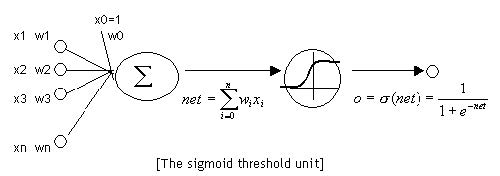
\includegraphics[width=0.7\textwidth]{Bp1.jpg}
	\caption{神经元}
	\label{fig:Bp1}
\end{figure}

计算一个神经元的输出的方法和计算一个感知器的输出是一样的。假设神经元的输入是向量\(\vec{x}\),权重向量是\(\vec{w}\)(偏置项是\(w_0\)),激活函数是sigmoid函数,则其输出\(y\):

\begin{equation}
	\label{eq:Bp1}
	y=sigmoid(\vec{w}^T\centerdot\vec{x})
\end{equation}


sigmoid函数的定义如下:
\[
	sigmoid(x)=\frac{1}{1+e^{-x}}
\]
将其带入前面的式子,得到
\[
	y=\frac{1}{1+e^{-\vec{w}^T\centerdot\vec{x}}}
\]
sigmoid函数是一个非线性函数,值域是(0,1)。函数图像如图\ref{fig:Bp2}所示

\begin{figure}[htbp]
	\centering
	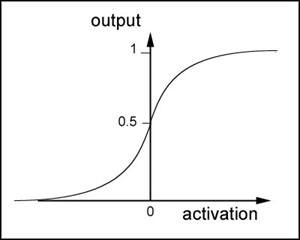
\includegraphics[width=0.5\textwidth]{Bp2.jpg}
	\caption{sigmoid函数}
	\label{fig:Bp2}
\end{figure}

sigmoid函数的导数是:
\begin{align*}
	 & \mbox{令} y=sigmoid(x) \\
	 & \mbox{则} y'=y(1-y)
\end{align*}


可以看到,sigmoid函数的导数非常有趣,它可以用sigmoid函数自身来表示。这样,一旦计算出sigmoid函数的值,计算它的导数的值就非常方便。


\section{神经网络是啥}\label{Bp:2}

\begin{figure}[htbp]
	\centering
	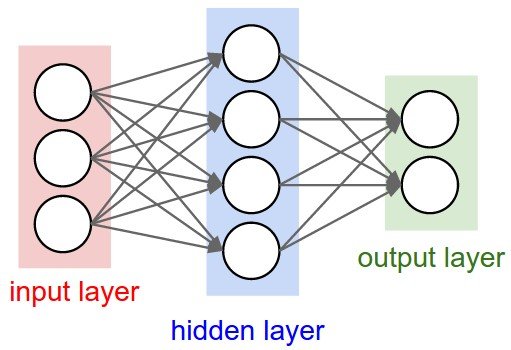
\includegraphics[width=0.5\textwidth]{Bp3.jpeg}
	\caption{Bp神经网络}
	\label{fig:Bp3}
\end{figure}

神经网络其实就是按照\textbf{一定规则}连接起来的多个\textbf{神经元}。图\ref{fig:Bp3}展示了一个\textbf{全连接(full connected, FC)}神经网络,通过观察可以发现它的规则包括:

\begin{itemize}
	\item
	      神经元按照\textbf{层}来布局。最左边的层叫做\textbf{输入层},负责接收输入数据;最右边的层叫\textbf{输出层},我们可以从这层获取神经网络输出数据。输入层和输出层之间的层叫做\textbf{隐藏层},因为它们对于外部来说是不可见的。
	\item
	      同一层的神经元之间没有连接。
	\item
	      第N层的每个神经元和第N-1层的\textbf{所有}神经元相连(这就是full connected的含义),第N-1层神经元的输出就是第N层神经元的输入。
	\item
	      每个连接都有一个\textbf{权值}。
\end{itemize}

上面这些规则定义了全连接神经网络的结构。事实上还存在很多其它结构的神经网络,比如卷积神经网络(CNN)、循环神经网络(RNN),他们都具有不同的连接规则。


\section{计算神经网络的输出}\label{Bp:3}

神经网络实际上就是一个输入向量\(\vec{x}\)到输出向量\(\vec{y}\)的函数,即:
\[
	\vec{y} = f_{network}(\vec{x})
\]

根据输入计算神经网络的输出,需要首先将输入向量\(\vec{x}\)的每个元素{}\(x_i\)的值赋给神经网络的输入层的对应神经元,然后根据公式\ref{eq:Bp1}依次向前计算每一层的每个神经元的值,直到最后一层输出层的所有神经元的值计算完毕。最后,将输出层每个神经元的值串在一起就得到了输出向量\(\vec{y}\)。

接下来举一个例子来说明这个过程,我们先给神经网络的每个单元写上编号。

\begin{figure}[htbp]
	\centering
	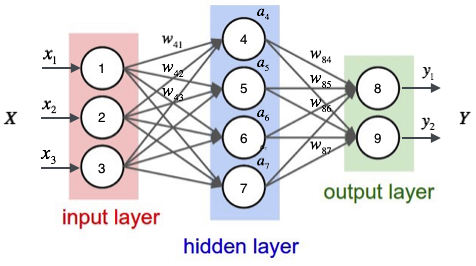
\includegraphics[width=0.7\textwidth]{Bp4.png}
	\caption{神经网络}
	\label{fig:Bp4}
\end{figure}

如上图,输入层有三个节点,我们将其依次编号为1、2、3;隐藏层的4个节点,编号依次为4、5、6、7;最后输出层的两个节点编号为8、9。因为我们这个神经网络是\textbf{全连接}网络,所以可以看到每个节点都和\textbf{上一层的所有节点}有连接。比如,我们可以看到隐藏层的节点4,它和输入层的三个节点1、2、3之间都有连接,其连接上的权重分别为\(w_{41},w_{42},w_{43}\)。那么,我们怎样计算节点4的输出值\(a_4\)呢?

为了计算节点4的输出值,我们必须先得到其所有上游节点(也就是节点1、2、3)的输出值。节点1、2、3是\textbf{输入层}的节点,所以,他们的输出值就是输入向量\(\vec{x}\)本身。按照上图画出的对应关系,可以看到节点1、2、3的输出值分别是\(x_1,x_2,x_3\)。我们要求\textbf{输入向量的维度和输入层神经元个数相同},而输入向量的某个元素对应到哪个输入节点是可以自由决定的,你偏非要把\(x_1\)赋值给节点2也是完全没有问题的,但这样除了把自己弄晕之外,并没有什么价值。

一旦我们有了节点1、2、3的输出值,我们就可以根据公式\ref{eq:Bp1}计算节点4的输出值\(a_4\):
\begin{align*}
	a_4 & =sigmoid(\vec{w}^T\centerdot\vec{x})           \\
	    & =sigmoid(w_{41}x_1+w_{42}x_2+w_{43}x_3+w_{4b})
\end{align*}


上式的\(w_{4b}\)是节点4的\textbf{偏置项},图中没有画出来。而\(w_{41},w_{42},w_{43}\)分别为节点1、2、3到节点4连接的权重,在给权重\(w_{ji}\)编号时,我们把目标节点的编号\(j\)放在前面,把源节点的编号\(i\)放在后面。

同样,我们可以继续计算出节点5、6、7的输出值\(a_5,a_6,a_7\)。这样,隐藏层的4个节点的输出值就计算完成了,我们就可以接着计算输出层的节点8的输出值\(y_1\):
\begin{align*}
	y_1 & =sigmoid(\vec{w}^T\centerdot\vec{a})                     \\
	    & =sigmoid(w_{84}a_4+w_{85}a_5+w_{86}a_6+w_{87}a_7+w_{8b})
\end{align*}

同理,我们还可以计算出\(y_2\)的值。这样输出层所有节点的输出值计算完毕,我们就得到了在输入向量\(\vec{x}=\begin{bmatrix}x_1\\x_2\\x_3\end{bmatrix}\)时,神经网络的输出向量\(\vec{y}=\begin{bmatrix}y_1\\y_2\end{bmatrix}\)。这里我们也看到,\textbf{输出向量的维度和输出层神经元个数相同}。


\section{神经网络的矩阵表示}\label{Bp:4}

神经网络的计算如果用矩阵来表示会很方便(当然逼格也更高),我们先来看看隐藏层的矩阵表示。

首先我们把隐藏层4个节点的计算依次排列出来:
\begin{align*}
	a_4 & =sigmoid(w_{41}x_1+w_{42}x_2+w_{43}x_3+w_{4b}) \\
	a_5 & =sigmoid(w_{51}x_1+w_{52}x_2+w_{53}x_3+w_{5b}) \\
	a_6 & =sigmoid(w_{61}x_1+w_{62}x_2+w_{63}x_3+w_{6b}) \\
	a_7 & =sigmoid(w_{71}x_1+w_{72}x_2+w_{73}x_3+w_{7b})
\end{align*}

接着,定义网络的输入向量\(\vec{x}\)和隐藏层每个节点的权重向量\(\vec{w_j}\)。令
\[\vec{x}=\begin{bmatrix}x_1\\x_2\\x_3\\1\end{bmatrix}\]
\begin{align*}
	\vec{w}_4 & =[w_{41},w_{42},w_{43},w_{4b}] \\
	\vec{w}_5 & =[w_{51},w_{52},w_{53},w_{5b}] \\
	\vec{w}_6 & =[w_{61},w_{62},w_{63},w_{6b}] \\
	\vec{w}_7 & =[w_{71},w_{72},w_{73},w_{7b}] \\
	f         & =sigmoid
\end{align*}


代入到前面的一组式子,得到:
\begin{align*}
	a_4 & =f(\vec{w_4}\centerdot\vec{x}),\qquad
	a_5=f(\vec{w_5}\centerdot\vec{x})           \\
	a_6 & =f(\vec{w_6}\centerdot\vec{x}),\qquad
	a_7=f(\vec{w_7}\centerdot\vec{x})
\end{align*}


现在,我们把上述计算\(a_4,a_5,a_6,a_7\)的四个式子写到一个矩阵里面,每个式子作为矩阵的一行,就可以利用矩阵来表示它们的计算了。令
\[
	\vec{a}=
	\begin{bmatrix}
		a_4 \\
		a_5 \\
		a_6 \\
		a_7 \\
	\end{bmatrix},\qquad W=
	\begin{bmatrix}
		\vec{w}_4 \\
		\vec{w}_5 \\
		\vec{w}_6 \\
		\vec{w}_7 \\
	\end{bmatrix}=
	\begin{bmatrix}
		w_{41},w_{42},w_{43},w_{4b} \\
		w_{51},w_{52},w_{53},w_{5b} \\
		w_{61},w_{62},w_{63},w_{6b} \\
		w_{71},w_{72},w_{73},w_{7b} \\
	\end{bmatrix}
	,\qquad f(
	\begin{bmatrix}
		x_1 \\
		x_2 \\
		x_3 \\
		.   \\
		.   \\
		.   \\
	\end{bmatrix})=
	\begin{bmatrix}
		f(x_1) \\
		f(x_2) \\
		f(x_3) \\
		.      \\
		.      \\
		.      \\
	\end{bmatrix}
\]

带入前面的一组式子,得到
\begin{equation}
	\label{eq:Bp2}
	\vec{a}=f(W\centerdot\vec{x})
\end{equation}

在公式\ref{eq:Bp2}中,\(f\)是激活函数,在本例中是\(sigmoid\)函数;\(W\)是某一层的权重矩阵;\(\vec{x}\)是某层的输入向量;\(\vec{a}\)是某层的输出向量。公式\ref{eq:Bp2}说明神经网络的每一层的作用实际上就是先将输入向量\textbf{左乘}一个数组进行线性变换,得到一个新的向量,然后再对这个向量\textbf{逐元素}应用一个激活函数。

每一层的算法都是一样的。比如,对于包含一个输入层,一个输出层和三个隐藏层的神经网络,我们假设其权重矩阵分别为\(W_1,W_2,W_3,W_4\),每个隐藏层的输出分别是\(\vec{a}_1,\vec{a}_2,\vec{a}_3\),神经网络的输入为\(\vec{x}\),神经网络的输入为\(\vec{y}\),如图\ref{fig:Bp5}所示:

\begin{figure}[htbp]
	\centering
	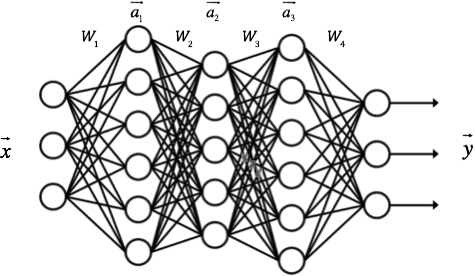
\includegraphics[width=0.7\textwidth]{Bp5.png}
	\caption{神经网络}
	\label{fig:Bp5}
\end{figure}

则每一层的输出向量的计算可以表示为:
\begin{align*}
	 & \vec{a}_1=f(W_1\centerdot\vec{x}),\qquad \vec{a}_2=f(W_2\centerdot\vec{a}_1) \\
	 & \vec{a}_3=f(W_3\centerdot\vec{a}_2),\qquad\vec{y}=f(W_4\centerdot\vec{a}_3)
\end{align*}


这就是神经网络输出值的计算方法。


\section{神经网络的训练}\label{Bp:5}

现在,我们需要知道一个神经网络的每个连接上的权值是如何得到的。我们可以说神经网络是一个\textbf{模型},那么这些权值就是模型的\textbf{参数},也就是模型要学习的东西。然而,一个神经网络的连接方式、网络的层数、每层的节点数这些参数,则不是学习出来的,而是人为事先设置的。对于这些人为设置的参数,我们称之为\textbf{超参数(Hyper-Parameters)}。

接下来,我们将要介绍神经网络的训练算法:反向传播算法。


\subsection{反向传播算法(Back Propagation)}\label{Bp:6}

我们首先直观的介绍反向传播算法,最后再来介绍这个算法的推导。当然读者也可以完全跳过推导部分,因为即使不知道如何推导,也不影响你写出来一个神经网络的训练代码。事实上,现在神经网络成熟的开源实现多如牛毛,除了练手之外,你可能都没有机会需要去写一个神经网络。

我们以\textbf{监督学习}为例来解释反向传播算法。在第\ref{chap:Line}章中我们介绍了什么是\textbf{监督学习},如果忘记了可以再看一下。另外,我们设神经元的激活函数\(f\)为\(sigmoid\)函数(不同激活函数的计算公式不同,详情见\ref{Bp:7}反向传播算法的推导一节)。

我们假设每个训练样本为\((\vec{x},\vec{t})\),其中向量\(\vec{x}\)是训练样本的特征,而\(\vec{t}\)是样本的目标值。

首先,我们根据上一节介绍的算法,用样本的特征\(\vec{x}\),计算出神经网络中每个隐藏层节点的输出\(a_i\),以及输出层每个节点的输出\(y_i\)。

然后,我们按照下面的方法计算出每个节点的误差项\(\delta_i\):

\begin{itemize}
	\item
	      对于输出层节点\(i\),
	      \begin{equation}
		      \label{eq:Bp3}
		      \delta_i=y_i(1-y_i)(t_i-y_i)
	      \end{equation}

\end{itemize}
其中,\(\delta_i\)是节点\(i\)的误差项,\(y_i\)是节点\(i\)的\textbf{输出值},\(t_i\)是样本对应于节点\(i\)的\textbf{目标值}。举个例子,根据上图,对于输出层节点8来说,它的输出值是\(y_1\),而样本的目标值是\(t_1\),带入上面的公式得到节点8的误差项\(\delta_8\)应该是:
\[
	\delta_8=y_1(1-y_1)(t_1-y_1)
\]

\begin{itemize}
	\item
	      对于隐藏层节点,
	      \begin{equation}
		      \label{eq:Bp4}
		      \delta_i=a_i(1-a_i)\sum_{k\in{outputs}}w_{ki}\delta_k
	      \end{equation}
\end{itemize}
其中,\(a_i\)是节点\(i\)的输出值,\(w_{ki}\)是节点\(i\)到它的下一层节点\(k\)的连接的权重,\(\delta_k\)是节点\(i\)的下一层节点\(k\)的误差项。例如,对于隐藏层节点4来说,计算方法如下:
\[
	\delta_4=a_4(1-a_4)(w_{84}\delta_8+w_{94}\delta_9)
\]
最后,更新每个连接上的权值:
\begin{equation}
	\label{eq:Bp5}
	w_{ji}\gets w_{ji}+\eta\delta_jx_{ji}
\end{equation}
其中,\(w_{ji}\)是节点\(i\)到节点\(j\)的权重,\(\eta\)是一个成为\textbf{学习速率}的常数,\(\delta_j\)是节点的误差项,\(x_{ji}\)是节点\(i\)传递给节点\(j\)的输入。例如,权重\(w_84\)的更新方法如下:
\[
	w_{84}\gets w_{84}+\eta\delta_8 a_4
\]
类似的,权重\(w_{41}\)的更新方法如下:
\[
	w_{41}\gets w_{41}+\eta\delta_4 x_1
\]

偏置项的输入值永远为1。例如,节点4的偏置项\(w_{4b}\)应该按照下面的方法计算:
\[
	w_{4b}\gets w_{4b}+\eta\delta_4
\]

我们已经介绍了神经网络每个节点误差项的计算和权重更新方法。显然,计算一个节点的误差项,需要先计算每个与其相连的下一层节点的误差项。这就要求误差项的计算顺序必须是从输出层开始,然后反向依次计算每个隐藏层的误差项,直到与输入层相连的那个隐藏层。这就是反向传播算法的名字的含义。当所有节点的误差项计算完毕后,我们就可以根据公式\ref{eq:Bp5}来更新所有的权重。

以上就是基本的反向传播算法,并不是很复杂,您弄清楚了么?




\subsection{反向传播算法的推导}\label{Bp:7}
反向传播算法其实就是链式求导法则的应用。然而,这个如此简单且显而易见的方法,却是在Roseblatt提出感知器算法将近30年之后才被发明和普及的。对此,Bengio这样回应道:

\begin{note}
	很多看似显而易见的想法只有在事后才变得显而易见。
\end{note}

接下来,我们用链式求导法则来推导反向传播算法,也就是上一小节的公式\ref{eq:Bp3}, \ref{eq:Bp4}, \ref{eq:Bp5}。

% \textbf{\emph{前方高能预警——接下来是数学公式重灾区,读者可以酌情阅读,不必强求。}}

按照机器学习的通用套路,我们先确定神经网络的目标函数,然后用\textbf{随机梯度下降}优化算法去求目标函数最小值时的参数值。

我们取网络所有输出层节点的误差平方和作为目标函数:
\[
	E_d\equiv\frac{1}{2}\sum_{i\in outputs}(t_i-y_i)^2
\]

其中,\(E_d\)表示是样本\(d\)的误差。

然后,我们用第\ref{chap:Line}章中介绍的\textbf{随机梯度下降}算法对目标函数进行优化:
\[
	w_{ji}\gets w_{ji}-\eta\frac{\partial{E_d}}{\partial{w_{ji}}}
\]

随机梯度下降算法也就是需要求出误差\(E_d\)对于每个权重\(w_{ji}\)的偏导数(也就是梯度),怎么求呢?观察图\ref{fig:Bp4},我们发现权重\(w_{ji}\)仅能通过影响节点\(j\)的输入值影响网络的其它部分,设\(net_j\)是节点\(j\)的\textbf{加权输入},即
\begin{align*}
	net_j=\vec{w_j}\centerdot\vec{x_j} =\sum_{i}{w_{ji}}x_{ji}
\end{align*}
\(E_d\)是\(net_j\)的函数,而\(net_j\)是\(w_{ji}\)的函数。根据链式求导法则,可以得到:
\begin{align*}
	\frac{\partial{E_d}}{\partial{w_{ji}}}=\frac{\partial{E_d}}{\partial{net_j}}\frac{\partial{net_j}}{\partial{w_{ji}}}=\frac{\partial{E_d}}{\partial{net_j}}\frac{\partial{\sum_{i}{w_{ji}}x_{ji}}}{\partial{w_{ji}}}=\frac{\partial{E_d}}{\partial{net_j}}x_{ji}
\end{align*}
上式中,\(x_{ji}\)是节点\(i\)传递给节点\(j\)的输入值,也就是节点\(i\)的输出值。

对于\(\frac{\partial{E_d}}{\partial{net_j}}\)的推导,需要区分\textbf{输出层}和\textbf{隐藏层}两种情况。


\textbf{输出层权值训练}

对于\textbf{输出层}来说,\(net_j\)仅能通过节点\(j\)的输出值\(y_j\)来影响网络其它部分,也就是说\(E_d\)是\(y_j\)的函数,而\(y_j\)是\(net_j\)的函数,其中\(y_j=sigmoid(net_j)\)。所以我们可以再次使用链式求导法则:
\begin{align*}
	\frac{\partial{E_d}}{\partial{net_j}} & =\frac{\partial{E_d}}{\partial{y_j}}\frac{\partial{y_j}}{\partial{net_j}}
\end{align*}


考虑上式第一项:
\begin{align*}
	\frac{\partial{E_d}}{\partial{y_j}} & =\frac{\partial}{\partial{y_j}}\frac{1}{2}\sum_{i\in outputs}(t_i-y_i)^2 \\
	                                    & =\frac{\partial}{\partial{y_j}}\frac{1}{2}(t_j-y_j)^2                    \\
	                                    & =-(t_j-y_j)
\end{align*}


考虑上式第二项:
\begin{align*}
	\frac{\partial{y_j}}{\partial{net_j}} & =\frac{\partial sigmoid(net_j)}{\partial{net_j}} \\
	                                      & =y_j(1-y_j)
\end{align*}


将第一项和第二项带入,得到:
\[
	\frac{\partial{E_d}}{\partial{net_j}}=-(t_j-y_j)y_j(1-y_j)
\]

如果令\(\delta_j=-\frac{\partial{E_d}}{\partial{net_j}}\),也就是一个节点的误差项\(\delta\)是网络误差对这个节点输入的偏导数的相反数。带入上式,得到:
\[
	\delta_j=(t_j-y_j)y_j(1-y_j)
\]

上式就是公式\ref{eq:Bp3}。

将上述推导带入随机梯度下降公式,得到:
\begin{align*}
	w_{ji} & \gets w_{ji}-\eta\frac{\partial{E_d}}{\partial{w_{ji}}} \\
	       & =w_{ji}+\eta(t_j-y_j)y_j(1-y_j)x_{ji}                   \\
	       & =w_{ji}+\eta\delta_jx_{ji}
\end{align*}


上式就是公式\ref{eq:Bp5}。

\textbf{隐藏层权值训练}

现在我们要推导出隐藏层的\(\frac{\partial{E_d}}{\partial{net_j}}\)。

首先,我们需要定义节点\(j\)的所有直接下游节点的集合\(Downstream(j)\)。例如,对于节点4来说,它的直接下游节点是节点8、节点9。可以看到\(net_j\)只能通过影响\(Downstream(j)\)再影响\(E_d\)。设\(net_k\)是节点\(j\)的下游节点的输入,则\(E_d\)是\(net_k\)的函数,而\(net_k\)是\(net_j\)的函数。因为\(net_k\)有多个,我们应用全导数公式,可以做出如下推导:
\begin{align*}
	\frac{\partial{E_d}}{\partial{net_j}} & =\sum_{k\in Downstream(j)}\frac{\partial{E_d}}{\partial{net_k}}\frac{\partial{net_k}}{\partial{net_j}}        \\
	                                      & =\sum_{k\in Downstream(j)}-\delta_k\frac{\partial{net_k}}{\partial{net_j}}                                    \\
	                                      & =\sum_{k\in Downstream(j)}-\delta_k\frac{\partial{net_k}}{\partial{a_j}}\frac{\partial{a_j}}{\partial{net_j}} \\
	                                      & =\sum_{k\in Downstream(j)}-\delta_kw_{kj}\frac{\partial{a_j}}{\partial{net_j}}                                \\
	                                      & =\sum_{k\in Downstream(j)}-\delta_kw_{kj}a_j(1-a_j)                                                           \\
	                                      & =-a_j(1-a_j)\sum_{k\in Downstream(j)}\delta_kw_{kj}
\end{align*}

因为\(\delta_j=-\frac{\partial{E_d}}{\partial{net_j}}\),带入上式得到:
\[
	\delta_j=a_j(1-a_j)\sum_{k\in Downstream(j)}\delta_kw_{kj}
\]

上式就是公式\ref{eq:Bp4}。

\textbf{——数学公式警报解除——}

至此,我们已经推导出了反向传播算法。需要注意的是,我们刚刚推导出的训练规则是根据激活函数是sigmoid函数、平方和误差、全连接网络、随机梯度下降优化算法。如果激活函数不同、误差计算方式不同、网络连接结构不同、优化算法不同,则具体的训练规则也会不一样。但是无论怎样,训练规则的推导方式都是一样的,应用链式求导法则进行推导即可。


\section{编程实战:神经网络的实现}\label{Bp:8}
\begin{note}
	完整代码请参考GitHub:\url{https://github.com/hanbt/learn_dl/blob/master/bp.py} (python2.7)
\end{note}

现在,我们要根据前面的算法,实现一个基本的全连接神经网络,这并不需要太多代码。我们在这里依然采用面向对象设计。

首先,我们先做一个基本的模型:

\begin{figure}[htbp]
	\centering
	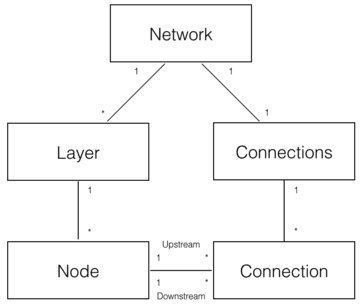
\includegraphics[width=0.4\textwidth]{Bp6.png}
	\caption{基础模型}
	\label{fig:Bp6}
\end{figure}
如图\ref{fig:Bp6},可以分解出5个领域对象来实现神经网络:
\begin{itemize}
	\item
	      \emph{Network}
	      神经网络对象,提供API接口。它由若干层对象组成以及连接对象组成。
	\item
	      \emph{Layer} 层对象,由多个节点组成。
	\item
	      \emph{Node} 节点对象计算和记录节点自身的信息(比如输出值\(a\)、误差项\(\delta\)等),以及与这个节点相关的上下游的连接。
	\item
	      \emph{Connection} 每个连接对象都要记录该连接的权重。
	\item
	      \emph{Connections} 仅仅作为Connection的集合对象,提供一些集合操作。
\end{itemize}

Node实现如下:
\begin{lstlisting}
# 节点类,负责记录和维护节点自身信息以及与这个节点相关的上下游连接,实现输出值和误差项的计算。
class Node(object):
    def __init__(self, layer_index, node_index):
        '''
        构造节点对象。
        layer_index: 节点所属的层的编号
        node_index: 节点的编号
        '''
        self.layer_index = layer_index
        self.node_index = node_index
        self.downstream = []
        self.upstream = []
        self.output = 0
        self.delta = 0
    def set_output(self, output):
        '''
        设置节点的输出值。如果节点属于输入层会用到这个函数。
        '''
        self.output = output
    def append_downstream_connection(self, conn):
        '''
        添加一个到下游节点的连接
        '''
        self.downstream.append(conn)
    def append_upstream_connection(self, conn):
        '''
        添加一个到上游节点的连接
        '''
        self.upstream.append(conn)
    def calc_output(self):
        '''
        根据式1计算节点的输出
        '''
        output = reduce(lambda ret, conn: ret + conn.upstream_node.output * conn.weight, self.upstream, 0)
        self.output = sigmoid(output)
    def calc_hidden_layer_delta(self):
        '''
        节点属于隐藏层时,根据式4计算delta
        '''
        downstream_delta = reduce(
            lambda ret, conn: ret + conn.downstream_node.delta * conn.weight,
            self.downstream, 0.0)
        self.delta = self.output * (1 - self.output) * downstream_delta
    def calc_output_layer_delta(self, label):
        '''
        节点属于输出层时,根据式3计算delta
        '''
        self.delta = self.output * (1 - self.output) * (label - self.output)
    def __str__(self):
        '''
        打印节点的信息
        '''
        node_str = '%u-%u: output: %f delta: %f' % (self.layer_index, self.node_index, self.output, self.delta)
        downstream_str = reduce(lambda ret, conn: ret + '\n\t' + str(conn), self.downstream, '')
        upstream_str = reduce(lambda ret, conn: ret + '\n\t' + str(conn), self.upstream, '')
        return node_str + '\n\tdownstream:' + downstream_str + '\n\tupstream:' + upstream_str 
\end{lstlisting}

ConstNode对象,为了实现一个输出恒为1的节点(计算偏置项\(w_b\)时需要)
\begin{lstlisting}
class ConstNode(object):
    def __init__(self, layer_index, node_index):
        '''
        构造节点对象。
        layer_index: 节点所属的层的编号
        node_index: 节点的编号
        '''    
        self.layer_index = layer_index
        self.node_index = node_index
        self.downstream = []
        self.output = 1
    def append_downstream_connection(self, conn):
        '''
        添加一个到下游节点的连接
        '''       
        self.downstream.append(conn)
    def calc_hidden_layer_delta(self):
        '''
        节点属于隐藏层时,根据式4计算delta
        '''
        downstream_delta = reduce(
            lambda ret, conn: ret + conn.downstream_node.delta * conn.weight,
            self.downstream, 0.0)
        self.delta = self.output * (1 - self.output) * downstream_delta
    def __str__(self):
        '''
        打印节点的信息
        '''
        node_str = '%u-%u: output: 1' % (self.layer_index, self.node_index)
        downstream_str = reduce(lambda ret, conn: ret + '\n\t' + str(conn), self.downstream, '')
        return node_str + '\n\tdownstream:' + downstream_str
\end{lstlisting}


Layer对象,负责初始化一层。此外,作为Node的集合对象,提供对Node集合的操作。
\begin{lstlisting}
class Layer(object):
    def __init__(self, layer_index, node_count):
        '''
        初始化一层
        layer_index: 层编号
        node_count: 层所包含的节点个数
        '''
        self.layer_index = layer_index
        self.nodes = []
        for i in range(node_count):
            self.nodes.append(Node(layer_index, i))
        self.nodes.append(ConstNode(layer_index, node_count))
    def set_output(self, data):
        '''
        设置层的输出。当层是输入层时会用到。
        '''
        for i in range(len(data)):
            self.nodes[i].set_output(data[i])
    def calc_output(self):
        '''
        计算层的输出向量
        '''
        for node in self.nodes[:-1]:
            node.calc_output()
    def dump(self):
        '''
        打印层的信息
        '''
        for node in self.nodes:
            print node
\end{lstlisting}

Connection对象,主要职责是记录连接的权重,以及这个连接所关联的上下游节点。
\begin{lstlisting}
class Connection(object):
    def __init__(self, upstream_node, downstream_node):
        '''
        初始化连接,权重初始化为是一个很小的随机数
        upstream_node: 连接的上游节点
        downstream_node: 连接的下游节点
        '''
        self.upstream_node = upstream_node
        self.downstream_node = downstream_node
        self.weight = random.uniform(-0.1, 0.1)
        self.gradient = 0.0
    def calc_gradient(self):
        '''
        计算梯度
        '''
        self.gradient = self.downstream_node.delta * self.upstream_node.output
    def get_gradient(self):
        '''
        获取当前的梯度
        '''
        return self.gradient
    def update_weight(self, rate):
        '''
        根据梯度下降算法更新权重
        '''
        self.calc_gradient()
        self.weight += rate * self.gradient
    def __str__(self):
        '''
        打印连接信息
        '''
        return '(%u-%u) -> (%u-%u) = %f' % (
            self.upstream_node.layer_index, 
            self.upstream_node.node_index,
            self.downstream_node.layer_index, 
            self.downstream_node.node_index, 
            self.weight)
\end{lstlisting}

Connections对象,提供Connection集合操作。
\begin{lstlisting}
class Connections(object):
    def __init__(self):
        self.connections = []
    def add_connection(self, connection):
        self.connections.append(connection)
    def dump(self):
        for conn in self.connections:
            print conn
\end{lstlisting}

Network对象,提供API。
\begin{lstlisting}
class Network(object):
    def __init__(self, layers):
        '''
        初始化一个全连接神经网络
        layers: 二维数组,描述神经网络每层节点数
        '''
        self.connections = Connections()
        self.layers = []
        layer_count = len(layers)
        node_count = 0;
        for i in range(layer_count):
            self.layers.append(Layer(i, layers[i]))
        for layer in range(layer_count - 1):
            connections = [Connection(upstream_node, downstream_node) 
                           for upstream_node in self.layers[layer].nodes
                           for downstream_node in self.layers[layer + 1].nodes[:-1]]
            for conn in connections:
                self.connections.add_connection(conn)
                conn.downstream_node.append_upstream_connection(conn)
                conn.upstream_node.append_downstream_connection(conn)
    def train(self, labels, data_set, rate, iteration):
        '''
        训练神经网络
        labels: 数组,训练样本标签。每个元素是一个样本的标签。
        data_set: 二维数组,训练样本特征。每个元素是一个样本的特征。
        '''
        for i in range(iteration):
            for d in range(len(data_set)):
                self.train_one_sample(labels[d], data_set[d], rate)
    def train_one_sample(self, label, sample, rate):
        '''
        内部函数,用一个样本训练网络
        '''
        self.predict(sample)
        self.calc_delta(label)
        self.update_weight(rate)
    def calc_delta(self, label):
        '''
        内部函数,计算每个节点的delta
        '''
        output_nodes = self.layers[-1].nodes
        for i in range(len(label)):
            output_nodes[i].calc_output_layer_delta(label[i])
        for layer in self.layers[-2::-1]:
            for node in layer.nodes:
                node.calc_hidden_layer_delta()
    def update_weight(self, rate):
        '''
        内部函数,更新每个连接权重
        '''
        for layer in self.layers[:-1]:
            for node in layer.nodes:
                for conn in node.downstream:
                    conn.update_weight(rate)
    def calc_gradient(self):
        '''
        内部函数,计算每个连接的梯度
        '''
        for layer in self.layers[:-1]:
            for node in layer.nodes:
                for conn in node.downstream:
                    conn.calc_gradient()
    def get_gradient(self, label, sample):
        '''
        获得网络在一个样本下,每个连接上的梯度
        label: 样本标签
        sample: 样本输入
        '''
        self.predict(sample)
        self.calc_delta(label)
        self.calc_gradient()
    def predict(self, sample):
        '''
        根据输入的样本预测输出值
        sample: 数组,样本的特征,也就是网络的输入向量
        '''
        self.layers[0].set_output(sample)
        for i in range(1, len(self.layers)):
            self.layers[i].calc_output()
        return map(lambda node: node.output, self.layers[-1].nodes[:-1])
    def dump(self):
        '''
        打印网络信息
        '''
        for layer in self.layers:
            layer.dump()
\end{lstlisting}

至此,实现了一个基本的全连接神经网络。可以看到,同神经网络的强大学习能力相比,其实现还算是很容易的。

\textbf{梯度检查}

怎么保证自己写的神经网络没有BUG呢?事实上这是一个非常重要的问题。一方面,千辛万苦想到一个算法,结果效果不理想,那么是算法本身错了还是代码实现错了呢?定位这种问题肯定要花费大量的时间和精力。另一方面,由于神经网络的复杂性,我们几乎无法事先知道神经网络的输入和输出,因此类似TDD(测试驱动开发)这样的开发方法似乎也不可行。

办法还是有滴,就是利用梯度检查来确认程序是否正确。梯度检查的思路如下:

对于梯度下降算法:
\[
	w_{ji}\gets w_{ji}-\eta\frac{\partial{E_d}}{\partial{w_{ji}}}
\]

来说,这里关键之处在于\(\frac{\partial{E_d}}{\partial{w_{ji}}}\)的计算一定要正确,而它是\(E_d\)对\(w_{ji}\)的\emph{偏导数}。而根据导数的定义:
\[
	f'(\theta)=\lim_{\epsilon->0}\frac{f(\theta+\epsilon)-f(\theta-\epsilon)}{2\epsilon}
\]

对于任意\(\theta\)的导数值,我们都可以用等式右边来近似计算。我们把\(E_d\)看做是\(w_{ji}\)的函数,即\(E_d(w_{ji})\),那么根据导数定义,\(\frac{\partial{E_d(w_{ji})}}{\partial{w_{ji}}}\)应该等于:
\[
	\frac{\partial{E_d(w_{ji})}}{\partial{w_{ji}}}=\lim_{\epsilon->0}\frac{f(w_{ji}+\epsilon)-f(w_{ji}-\epsilon)}{2\epsilon}
\]

如果把\(\epsilon\)设置为一个很小的数(比如\(10^{-4}\)),那么上式可以写成:
\begin{equation}
	\label{eq:Bp6}
	\frac{\partial{E_d(w_{ji})}}{\partial{w_{ji}}}\approx\frac{f(w_{ji}+\epsilon)-f(w_{ji}-\epsilon)}{2\epsilon}
\end{equation}


我们就可以利用公式\ref{eq:Bp6},来计算梯度\(\frac{\partial{E_d}}{\partial{w_{ji}}}\)的值,然后同我们神经网络代码中计算出来的梯度值进行比较。如果两者的差别\textbf{非常的小},那么就说明我们的代码是正确的。

下面是梯度检查的代码。如果我们想检查参数\(w_{ji}\)的梯度是否正确,我们需要以下几个步骤:

\begin{enumerate}
	\item
	      首先使用一个样本\(d\)对神经网络进行训练,这样就能获得每个权重的梯度。
	\item
	      将\(w_{ji}\)加上一个很小的值(\(10^{-4}\)),重新计算神经网络在这个样本\(d\)下的\(E_{d+}\)。
	\item
	      将\(w_{ji}\)减上一个很小的值(\(10^{-4}\)),重新计算神经网络在这个样本\(d\)下的\(E_{d-}\)。
	\item
	      根据公式\ref{eq:Bp6}计算出期望的梯度值,和第一步获得的梯度值进行比较,它们应该几乎想等(至少4位有效数字相同)。
\end{enumerate}

当然,我们可以重复上面的过程,对每个权重\(w_{ji}\)都进行检查。也可以使用多个样本重复检查。
\begin{lstlisting}
def gradient_check(network, sample_feature, sample_label):
    '''
    梯度检查
    network: 神经网络对象
    sample_feature: 样本的特征
    sample_label: 样本的标签
    '''
    # 计算网络误差
    network_error = lambda vec1, vec2: \
            0.5 * reduce(lambda a, b: a + b, 
                      map(lambda v: (v[0] - v[1]) * (v[0] - v[1]),
                          zip(vec1, vec2)))
    # 获取网络在当前样本下每个连接的梯度
    network.get_gradient(sample_feature, sample_label)
    # 对每个权重做梯度检查    
    for conn in network.connections.connections: 
        # 获取指定连接的梯度
        actual_gradient = conn.get_gradient()
        # 增加一个很小的值,计算网络的误差
        epsilon = 0.0001
        conn.weight += epsilon
        error1 = network_error(network.predict(sample_feature), sample_label)
        # 减去一个很小的值,计算网络的误差
        conn.weight -= 2 * epsilon # 刚才加过了一次,因此这里需要减去2倍
        error2 = network_error(network.predict(sample_feature), sample_label)
        # 根据式6计算期望的梯度值
        expected_gradient = (error2 - error1) / (2 * epsilon)
        # 打印
        print 'expected gradient: \t%f\nactual gradient: \t%f' % (
            expected_gradient, actual_gradient)
\end{lstlisting}

至此,会推导、会实现、会抓BUG,你已经摸到深度学习的大门了。接下来还需要不断的实践,我们用刚刚写过的神经网络去识别手写数字。


\section{神经网络实战:手写数字识别}\label{Bp:9}
针对这个任务,我们采用业界非常流行的MNIST数据集。MNIST大约有60000个手写字母的训练样本,我们使用它训练我们的神经网络,然后再用训练好的网络去识别手写数字。

手写数字识别是个比较简单的任务,数字只可能是0-9中的一个,这是个10分类问题。

\subsection{超参数的确定}\label{Bp:10}

我们首先需要确定网络的层数和每层的节点数。关于第一个问题,实际上并没有什么理论化的方法,大家都是根据经验来拍,如果没有经验的话就随便拍一个。然后,你可以多试几个值,训练不同层数的神经网络,看看哪个效果最好就用哪个。嗯,现在你可能明白为什么说深度学习是个手艺活了,有些手艺很让人无语,而有些手艺还是很有技术含量的。

不过,有些基本道理我们还是明白的,我们知道网络层数越多越好,也知道层数越多训练难度越大。对于全连接网络,隐藏层最好不要超过三层。那么,我们可以先试试仅有一个隐藏层的神经网络效果怎么样。毕竟模型小的话,训练起来也快些(刚开始玩模型的时候,都希望快点看到结果)。

输入层节点数是确定的。因为MNIST数据集每个训练数据是28*28的图片,共784个像素,因此,输入层节点数应该是784,每个像素对应一个输入节点。

输出层节点数也是确定的。因为是10分类,我们可以用10个节点,每个节点对应一个分类。输出层10个节点中,输出最大值的那个节点对应的分类,就是模型的预测结果。

隐藏层节点数量是不好确定的,从1到100万都可以。下面有几个经验公式:
\begin{align*}
	 & m=\sqrt{n+l}+\alpha \\
	 & m=log_2n            \\
	 & m=\sqrt{nl}
\end{align*}
其中,$m$:隐藏层节点数;$n$:输入层节点数;$l$:输出层节点数;$\alpha$:1到10之间的常数。
因此,我们可以先根据上面的公式设置一个隐藏层节点数。如果有时间,我们可以设置不同的节点数,分别训练,看看哪个效果最好就用哪个。我们先拍一个,设隐藏层节点数为300吧。

对于3层\(784*300*10\)的全连接网络,总共有\(300*(784+1)+10*(300+1)=238510\)个参数!神经网络之所以强大,是它提供了一种非常简单的方法去实现大量的参数。目前百亿参数、千亿样本的超大规模神经网络也是有的。因为MNIST只有6万个训练样本,参数太多了很容易过拟合,效果反而不好。

\subsection{模型的训练和评估}\label{Bp:11}

MNIST数据集包含10000个测试样本。我们先用60000个训练样本训练我们的网络,然后再用测试样本对网络进行测试,计算识别错误率:
\[
	\mbox{错误率}=\frac{\mbox{错误预测样本数}}{\mbox{总样本数}}
\]

我们每训练10轮,评估一次准确率。当准确率开始下降时(出现了过拟合)终止训练。


\subsection{代码实现}\label{Bp:12}

首先,我们需要把MNIST数据集处理为神经网络能够接受的形式。MNIST训练集的文件格式可以参考官方网站,这里不在赘述。每个训练样本是一个28*28的图像,我们按照行优先,把它转化为一个784维的向量。每个标签是0-9的值,我们将其转换为一个10维的one-hot向量:如果标签值为\(n\),我们就把向量的第\(n\)维(从0开始编号)设置为0.9,而其它维设置为0.1。例如,向量$[0.1,0.1,0.9,0.1,0.1,0.1,0.1,0.1,0.1,0.1]$表示值2。

下面是处理MNIST数据的代码:
\begin{lstlisting}
#!/usr/bin/env python
# -*- coding: UTF-8 -*-
import struct
from bp import *
from datetime import datetime
# 数据加载器基类
class Loader(object):
    def __init__(self, path, count):
        '''
        初始化加载器
        path: 数据文件路径
        count: 文件中的样本个数
        '''
        self.path = path
        self.count = count
    def get_file_content(self):
        '''
        读取文件内容
        '''
        f = open(self.path, 'rb')
        content = f.read()
        f.close()
        return content
    def to_int(self, byte):
        '''
        将unsigned byte字符转换为整数
        '''
        return struct.unpack('B', byte)[0]
# 图像数据加载器
class ImageLoader(Loader):
    def get_picture(self, content, index):
        '''
        内部函数,从文件中获取图像
        '''
        start = index * 28 * 28 + 16
        picture = []
        for i in range(28):
            picture.append([])
            for j in range(28):
                picture[i].append(
                    self.to_int(content[start + i * 28 + j]))
        return picture
    def get_one_sample(self, picture):
        '''
        内部函数,将图像转化为样本的输入向量
        '''
        sample = []
        for i in range(28):
            for j in range(28):
                sample.append(picture[i][j])
        return sample
    def load(self):
        '''
        加载数据文件,获得全部样本的输入向量
        '''
        content = self.get_file_content()
        data_set = []
        for index in range(self.count):
            data_set.append(
                self.get_one_sample(
                    self.get_picture(content, index)))
        return data_set
# 标签数据加载器
class LabelLoader(Loader):
    def load(self):
        '''
        加载数据文件,获得全部样本的标签向量
        '''
        content = self.get_file_content()
        labels = []
        for index in range(self.count):
            labels.append(self.norm(content[index + 8]))
        return labels
    def norm(self, label):
        '''
        内部函数,将一个值转换为10维标签向量
        '''
        label_vec = []
        label_value = self.to_int(label)
        for i in range(10):
            if i == label_value:
                label_vec.append(0.9)
            else:
                label_vec.append(0.1)
        return label_vec
def get_training_data_set():
    '''
    获得训练数据集
    '''
    image_loader = ImageLoader('train-images-idx3-ubyte', 60000)
    label_loader = LabelLoader('train-labels-idx1-ubyte', 60000)
    return image_loader.load(), label_loader.load()
def get_test_data_set():
    '''
    获得测试数据集
    '''
    image_loader = ImageLoader('t10k-images-idx3-ubyte', 10000)
    label_loader = LabelLoader('t10k-labels-idx1-ubyte', 10000)
    return image_loader.load(), label_loader.load()
\end{lstlisting}


网络的输出是一个10维向量,这个向量第\(n\)个(从0开始编号)元素的值最大,那么\(n\)就是网络的识别结果。下面是代码实现:
\begin{lstlisting}
def get_result(vec):
    max_value_index = 0
    max_value = 0
    for i in range(len(vec)):
        if vec[i] > max_value:
            max_value = vec[i]
            max_value_index = i
    return max_value_index
\end{lstlisting}

我们使用错误率来对网络进行评估,下面是代码实现:
\begin{lstlisting}
def evaluate(network, test_data_set, test_labels):
    error = 0
    total = len(test_data_set)
    for i in range(total):
        label = get_result(test_labels[i])
        predict = get_result(network.predict(test_data_set[i]))
        if label != predict:
            error += 1
    return float(error) / float(total)
\end{lstlisting}

最后实现我们的训练策略:每训练10轮,评估一次准确率,当准确率开始下降时终止训练。下面是代码实现:
\begin{lstlisting}
def train_and_evaluate():
    last_error_ratio = 1.0
    epoch = 0
    train_data_set, train_labels = get_training_data_set()
    test_data_set, test_labels = get_test_data_set()
    network = Network([784, 300, 10])
    while True:
        epoch += 1
        network.train(train_labels, train_data_set, 0.3, 1)
        print '%s epoch %d finished' % (now(), epoch)
        if epoch % 10 == 0:
            error_ratio = evaluate(network, test_data_set, test_labels)
            print '%s after epoch %d, error ratio is %f' % (now(), epoch, error_ratio)
            if error_ratio > last_error_ratio:
                break
            else:
                last_error_ratio = error_ratio
if __name__ == '__main__':
    train_and_evaluate()
\end{lstlisting}

在我的机器上测试了一下,1个epoch大约需要9000多秒,所以要对代码做很多的性能优化工作(比如用向量化编程)。训练要很久很久,可以把它上传到服务器上,在tmux的session里面去运行。为了防止异常终止导致前功尽弃,我们每训练10轮,就把获得参数值保存在磁盘上,以便后续可以恢复。(代码略)

\subsection{向量化编程}\label{Bp:13}

\begin{note}
	完整代码请参考GitHub:\url{https://github.com/hanbt/learn_dl/blob/master/fc.py} (python2.7)
\end{note}

在经历了漫长的训练之后,我们可能会想到,肯定有更好的办法!是的,程序员们,现在我们需要告别面向对象编程了,转而去使用另外一种更适合深度学习算法的编程方式:向量化编程。主要有两个原因:一个是我们事实上并不需要真的去定义Node、Connection这样的对象,直接把数学计算实现了就可以了;另一个原因,是底层算法库会针对向量运算做优化(甚至有专用的硬件,比如GPU),程序效率会提升很多。所以,在深度学习的世界里,我们总会想法设法的把计算表达为向量的形式。我相信优秀的程序员不会把自己拘泥于某种(自己熟悉的)编程范式上,而会去学习并使用最为合适的范式。

下面,我们用向量化编程的方法,重新实现前面的\textbf{全连接神经网络}。

首先,我们需要把所有的计算都表达为向量的形式。对于全连接神经网络来说,主要有三个计算公式。

前向计算,我们发现公式\ref{eq:Bp2}已经是向量化的表达了:
\begin{equation}
	\label{eq:Bp2_1}
	\vec{a}=\sigma(W\centerdot\vec{x})
\end{equation}

上式中的\(\sigma\)表示sigmoid函数。

反向计算,我们需要把公式\ref{eq:Bp3}和公式\ref{eq:Bp4}使用向量来表示:
\begin{align}
	\vec{\delta}       & =\vec{y}(1-\vec{y})(\vec{t}-\vec{y}) \label{eq:Bp7}             \\
	\vec{\delta^{(l)}} & =\vec{a}^{(l)}(1-\vec{a}^{(l)})W^T\delta^{(l+1)} \label{eq:Bp8}
\end{align}


在公式\ref{eq:Bp8}中,\(\delta^{(l)}\)表示第l层的误差项;\(W^T\)表示矩阵\(W\)的转置。

我们还需要权重数组W和偏置项b的梯度计算的向量化表示。也就是需要把公式\ref{eq:Bp5}使用向量化表示:
\begin{equation}
	\label{eq:Bp5_1}
	w_{ji}\gets w_{ji}+\eta\delta_jx_{ji}
\end{equation}

其对应的向量化表示为:
\begin{equation}
	\label{eq:Bp9}
	W \gets W + \eta\vec{\delta}\vec{x}^T
\end{equation}

更新偏置项的向量化表示为:
\begin{equation}
	\label{eq:Bp10}
	\vec{b} \gets \vec{b} + \eta\vec{\delta}
\end{equation}

现在,我们根据上面几个公式,重新实现一个类:FullConnectedLayer。它实现了全连接层的前向和后向计算:
\begin{lstlisting}
# 全连接层实现类
class FullConnectedLayer(object):
    def __init__(self, input_size, output_size, 
                 activator):
        '''
        构造函数
        input_size: 本层输入向量的维度
        output_size: 本层输出向量的维度
        activator: 激活函数
        '''
        self.input_size = input_size
        self.output_size = output_size
        self.activator = activator
        # 权重数组W
        self.W = np.random.uniform(-0.1, 0.1,
            (output_size, input_size))
        # 偏置项b
        self.b = np.zeros((output_size, 1))
        # 输出向量
        self.output = np.zeros((output_size, 1))
    def forward(self, input_array):
        '''
        前向计算
        input_array: 输入向量,维度必须等于input_size
        '''
        # 式2
        self.input = input_array
        self.output = self.activator.forward(
            np.dot(self.W, input_array) + self.b)
    def backward(self, delta_array):
        '''
        反向计算W和b的梯度
        delta_array: 从上一层传递过来的误差项
        '''
        # 式8
        self.delta = self.activator.backward(self.input) * np.dot(
            self.W.T, delta_array)
        self.W_grad = np.dot(delta_array, self.input.T)
        self.b_grad = delta_array
    def update(self, learning_rate):
        '''
        使用梯度下降算法更新权重
        '''
        self.W += learning_rate * self.W_grad
        self.b += learning_rate * self.b_grad
\end{lstlisting}


上面这个类一举取代了原先的Layer、Node、Connection等类,不但代码更加容易理解,而且运行速度也快了几百倍。

现在,我们对Network类稍作修改,使之用到FullConnectedLayer:
\begin{lstlisting}
# Sigmoid激活函数类
class SigmoidActivator(object):
    def forward(self, weighted_input):
        return 1.0 / (1.0 + np.exp(-weighted_input))
    def backward(self, output):
        return output * (1 - output)
# 神经网络类
class Network(object):
    def __init__(self, layers):
        '''
        构造函数
        '''
        self.layers = []
        for i in range(len(layers) - 1):
            self.layers.append(
                FullConnectedLayer(
                    layers[i], layers[i+1],
                    SigmoidActivator()
                )
            )
    def predict(self, sample):
        '''
        使用神经网络实现预测
        sample: 输入样本
        '''
        output = sample
        for layer in self.layers:
            layer.forward(output)
            output = layer.output
        return output
    def train(self, labels, data_set, rate, epoch):
        '''
        训练函数
        labels: 样本标签
        data_set: 输入样本
        rate: 学习速率
        epoch: 训练轮数
        '''
        for i in range(epoch):
            for d in range(len(data_set)):
                self.train_one_sample(labels[d], 
                    data_set[d], rate)
    def train_one_sample(self, label, sample, rate):
        self.predict(sample)
        self.calc_gradient(label)
        self.update_weight(rate)
    def calc_gradient(self, label):
        delta = self.layers[-1].activator.backward(
            self.layers[-1].output
        ) * (label - self.layers[-1].output)
        for layer in self.layers[::-1]:
            layer.backward(delta)
            delta = layer.delta
        return delta
    def update_weight(self, rate):
        for layer in self.layers:
            layer.update(rate)
\end{lstlisting}

现在,Network类也清爽多了,用我们的新代码再次训练一下MNIST数据集吧。

\section{小结}

至此,你已经完成了又一次漫长的学习之旅。你现在应该已经明白了神经网络的基本原理,高兴的话,你甚至有能力去动手实现一个,并用它解决一些问题。如果感到困难也不要气馁,这篇文章是一个重要的分水岭,如果你完全弄明白了的话,在真正的『小白』和装腔作势的『大牛』面前吹吹牛是完全没有问题的。

作为深度学习入门的系列文章,本文也是上半场的结束。在这个半场,你掌握了机器学习、神经网络的\textbf{基本}概念,并且有能力去动手解决一些简单的问题(例如手写数字识别,如果用传统的观点来看,其实这些问题也不简单)。而且,一旦掌握基本概念,后面的学习就容易多了。

在下半场,我们讲介绍更多『深度』学习的内容,我们已经讲了神经网络(Neutrol Network),但是并没有讲深度神经网络(Deep Neutrol Network)。Deep会带来更加强大的能力,同时也带来更多的问题。如果不理解这些问题和它们的解决方案,也不能说你入门了『深度』学习。

目前业界有很多开源的神经网络实现,它们的功能也要强大的多,因此你并不需要事必躬亲的去实现自己的神经网络。我们在上半场不断的从头发明轮子,是为了让你明白神经网络的基本原理,这样你就能非常迅速的掌握这些工具。在下半场的文章中,我们改变了策略:不会再去从头开始去实现,而是尽可能应用现有的工具。

下一篇文章,我们介绍不同结构的神经网络,比如鼎鼎大名的\textbf{卷积神经网络},它在图像和语音领域已然创造了诸多奇迹,在自然语言处理领域的研究也如火如荼。某种意义上说,它的成功大大提升了人们对于深度学习的信心。



\chapter{卷积神经网络}\label{chap:Cnn}

\begin{introduction}
	\item 激活函数:Relu~\ref{Cnn:1}
	\item 全连接网络 VS 卷积网络~\ref{Cnn:2}
	\item 卷积神经网络是啥~\ref{Cnn:3}
	\item 卷积神经网络输出值的计算~\ref{Cnn:4}
	\item 卷积层输出值的计算~\ref{Cnn:5}
	\item Pooling层输出值的计算~\ref{Cnn:6}
	\item 卷积神经网络的训练~\ref{Cnn:7}
	\item 卷积层的训练~\ref{Cnn:8}
	\item Pooling层的训练~\ref{Cnn:9}
	\item 编程实战:卷积神经网络的实现~\ref{Cnn:10}
	\item 卷积层的实现~\ref{Cnn:11}
	\item Max Pooling层的实现~\ref{Cnn:12}
	\item 卷积神经网络的应用~\ref{Cnn:13}
\end{introduction}

在前面的文章中,我们介绍了全连接神经网络,以及它的训练和使用。我们用它来识别了手写数字,然而,这种结构的网络对于图像识别任务来说并不是很合适。本文将要介绍一种更适合图像、语音识别任务的神经网络结构------\textbf{卷积神经网络}(Convolutional Neural Network,
CNN)。说卷积神经网络是最重要的一种神经网络也不为过,它在最近几年大放异彩,几乎所有图像、语音识别领域的重要突破都是卷积神经网络取得的,比如谷歌的GoogleNet、微软的ResNet等,打败李世石的AlphaGo也用到了这种网络。本文将详细介绍\textbf{卷积神经网络}以及它的训练算法,以及动手实现一个简单的\textbf{卷积神经网络}。

\section{激活函数:Relu}\label{Cnn:1}

最近几年卷积神经网络中,激活函数往往不选择sigmoid或tanh函数,而是选择relu函数。Relu函数的定义是:
\[
	f(x)= max(0,x)
\]

Relu函数图像如图\ref{fig:Cnn1}所示:
\begin{figure}[!h]
	\centering
	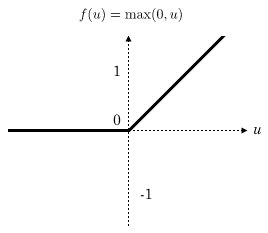
\includegraphics[width=0.45\textwidth]{Cnn1.png}
	\caption{Relu函数}
	\label{fig:Cnn1}
\end{figure}


Relu函数作为激活函数,有下面几大优势:

\begin{itemize}
	\item
	      \textbf{速度快}
	      和sigmoid函数需要计算指数和倒数相比,relu函数其实就是一个max(0,x),计算代价小很多。
	\item
	      \textbf{减轻梯度消失问题}
	      回忆一下计算梯度的公式\(\nabla=\sigma'\delta x\)。其中,\(\sigma'\)是sigmoid函数的导数。在使用反向传播算法进行梯度计算时,每经过一层sigmoid神经元,梯度就要乘上一个\(\sigma'\)。从下图可以看出,\(\sigma'\)函数最大值是1/4。因此,乘一个\(\sigma'\)会导致梯度越来越小,这对于深层网络的训练是个很大的问题。而relu函数的导数是1,不会导致梯度变小。当然,激活函数仅仅是导致梯度减小的一个因素,但无论如何在这方面relu的表现强于sigmoid。使用relu激活函数可以让你训练更深的网络。
	\item
	      \textbf{稀疏性}
	      通过对大脑的研究发现,大脑在工作的时候只有大约5\%的神经元是激活的,而采用sigmoid激活函数的人工神经网络,其激活率大约是50\%。有论文声称人工神经网络在15\%-30\%的激活率时是比较理想的。因为relu函数在输入小于0时是完全不激活的,因此可以获得一个更低的激活率。
\end{itemize}

\begin{figure}[htbp]
	\centering
	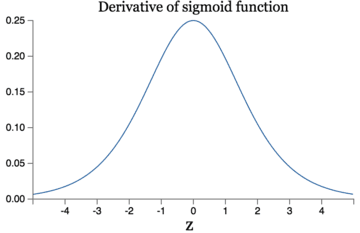
\includegraphics[width=0.6\textwidth]{Cnn2.png}
	\caption{Relu函数导数}
	\label{fig:Cnn2}
\end{figure}



\section{全连接网络 VS 卷积网络}\label{Cnn:2}


全连接神经网络之所以不太适合图像识别任务,主要有以下几个方面的问题:

\begin{itemize}
	\item
	      \textbf{参数数量太多}
	      考虑一个输入1000*1000像素的图片(一百万像素,现在已经不能算大图了),输入层有1000*1000=100万节点。假设第一个隐藏层有100个节点(这个数量并不多),那么仅这一层就有(1000*1000+1)*100=1亿参数,这实在是太多了!我们看到图像只扩大一点,参数数量就会多很多,因此它的扩展性很差。
	\item
	      \textbf{没有利用像素之间的位置信息}
	      对于图像识别任务来说,每个像素和其周围像素的联系是比较紧密的,和离得很远的像素的联系可能就很小了。如果一个神经元和上一层所有神经元相连,那么就相当于对于一个像素来说,把图像的所有像素都等同看待,这不符合前面的假设。当我们完成每个连接权重的学习之后,最终可能会发现,有大量的权重,它们的值都是很小的(也就是这些连接其实无关紧要)。努力学习大量并不重要的权重,这样的学习必将是非常低效的。
	\item
	      \textbf{网络层数限制}
	      我们知道网络层数越多其表达能力越强,但是通过梯度下降方法训练深度全连接神经网络很困难,因为全连接神经网络的梯度很难传递超过3层。因此,我们不可能得到一个很深的全连接神经网络,也就限制了它的能力。
\end{itemize}

那么,卷积神经网络又是怎样解决这个问题的呢?主要有三个思路:

\begin{itemize}
	\item
	      \textbf{局部连接}
	      这个是最容易想到的,每个神经元不再和上一层的所有神经元相连,而只和一小部分神经元相连。这样就减少了很多参数。
	\item
	      \textbf{权值共享}
	      一组连接可以共享同一个权重,而不是每个连接有一个不同的权重,这样又减少了很多参数。
	\item
	      \textbf{下采样}
	      可以使用Pooling来减少每层的样本数,进一步减少参数数量,同时还可以提升模型的鲁棒性。
\end{itemize}

对于图像识别任务来说,卷积神经网络通过尽可能保留重要的参数,去掉大量不重要的参数,来达到更好的学习效果。

接下来,我们将详述卷积神经网络到底是何方神圣。


\section{卷积神经网络是啥}\label{Cnn:3}
首先,我们先获取一个感性认识,图\ref{fig:Cnn3}是一个卷积神经网络的示意图:

\begin{figure}[htbp]
	\centering
	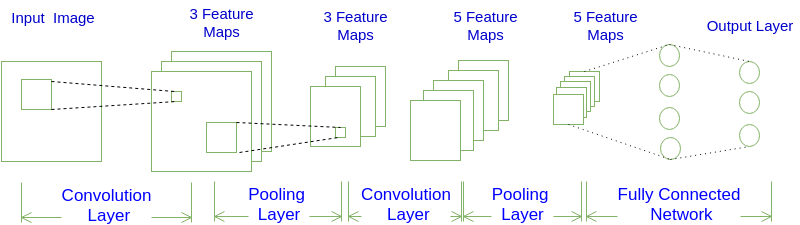
\includegraphics[width=1\textwidth]{Cnn3.png}
	\caption{卷积神经网络}
	\label{fig:Cnn3}
\end{figure}

\subsection{网络架构}

如图\ref{fig:Cnn3}所示,一个卷积神经网络由若干\textbf{卷积层}、\textbf{Pooling层}、\textbf{全连接层}组成。你可以构建各种不同的卷积神经网络,它的常用架构模式为:
\begin{lstlisting}[numbers=none]
    INPUT -> [[CONV]*N -> POOL?]*M -> [FC]*K
\end{lstlisting}

也就是N个卷积层叠加,然后(可选)叠加一个Pooling层,重复这个结构M次,最后叠加K个全连接层。

对于图\ref{fig:Cnn3}展示的卷积神经网络:
\begin{lstlisting}[numbers=none]
    INPUT -> CONV -> POOL -> CONV -> POOL -> FC -> FC
\end{lstlisting}

按照上述模式可以表示为:
\begin{lstlisting}[numbers=none]
    INPUT -> [[CONV]*1 -> POOL]*2 -> [FC]*2
\end{lstlisting}

也就是:\texttt{N=1,\ M=2,\ K=2}。

\subsection{三维的层结构}

从图\ref{fig:Cnn3}我们可以发现\textbf{卷积神经网络}的层结构和\textbf{全连接神经网络}的层结构有很大不同。\textbf{全连接神经网络}每层的神经元是按照\textbf{一维}排列的,也就是排成一条线的样子;而\textbf{卷积神经网络}每层的神经元是按照\textbf{三维}排列的,也就是排成一个长方体的样子,有\textbf{宽度}、\textbf{高度}和\textbf{深度}。

对于图\ref{fig:Cnn3}展示的神经网络,我们看到输入层的宽度和高度对应于输入图像的宽度和高度,而它的深度为1。接着,第一个卷积层对这幅图像进行了卷积操作(后面我们会讲如何计算卷积),得到了三个Feature Map。这里的"3"可能是让很多初学者迷惑的地方,实际上,就是这个卷积层包含三个Filter,也就是三套参数,每个Filter都可以把原始输入图像卷积得到一个Feature Map,三个Filter就可以得到三个Feature Map。至于一个卷积层可以有多少个Filter,那是可以自由设定的。也就是说,卷积层的Filter个数也是一个\textbf{超参数}。我们可以把Feature Map可以看做是通过卷积变换提取到的图像特征,三个Filter就对原始图像提取出三组不同的特征,也就是得到了三个Feature Map,也称做三个\textbf{通道(channel)}。

继续观察图\ref{fig:Cnn3},在第一个卷积层之后,Pooling层对三个Feature Map做了\textbf{下采样}(后面我们会讲如何计算下采样),得到了三个更小的Feature Map。接着,是第二个\textbf{卷积层},它有5个Filter。每个Fitler都把前面\textbf{下采样}之后的\textbf{3个Feature Map}卷积\textbf{在一起,得到一个新的Feature Map。这样,5个Filter就得到了5个Feature Map。接着,是第二个Pooling,继续对5个Feature Map进行}下采样,得到了5个更小的Feature Map。

图\ref{fig:Cnn3}所示网络的最后两层是全连接层。第一个全连接层的每个神经元,和上一层5个Feature Map中的每个神经元相连,第二个全连接层(也就是输出层)的每个神经元,则和第一个全连接层的每个神经元相连,这样得到了整个网络的输出。

至此,我们对\textbf{卷积神经网络}有了最基本的感性认识。接下来,我们将介绍\textbf{卷积神经网络}中各种层的计算和训练。


\section{卷积神经网络输出值的计算}\label{Cnn:4}
\subsection{卷积层输出值的计算}\label{Cnn:5}

我们用一个简单的例子来讲述如何计算\textbf{卷积},然后,我们抽象出\textbf{卷积层}的一些重要概念和计算方法。

\begin{figure}[!h]
	\centering
	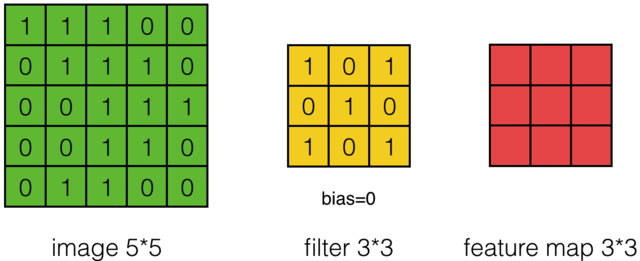
\includegraphics[width=0.8\textwidth]{Cnn4.png}
	\caption{Feature Map}
	\label{fig:Cnn4}
\end{figure}

假设有一个5*5的图像,使用一个3*3的filter进行卷积,想得到一个3*3的Feature Map,如图\ref{fig:Cnn4}所示。为了清楚的描述\textbf{卷积}计算过程,我们首先对图像的每个像素进行编号,用\(x_{i,j}\)表示图像的第\(i\)行第\(j\)列元素;对filter的每个权重进行编号,用\(w_{m,n}\)表示第\(m\)行第\(n\)列权重,用\(w_b\)表示filter的\textbf{偏置项};对Feature Map的每个元素进行编号,用\(a_{i,j}\)表示Feature Map的第\(i\)行第\(j\)列元素;用\(f\)表示\textbf{激活函数}(这个例子选择\textbf{relu函数}作为激活函数)。然后,使用下列公式计算卷积:

\begin{equation}
	\label{eq:Cnn1}
	a_{i,j}=f(\sum_{m=0}^{2}\sum_{n=0}^{2}w_{m,n}x_{i+m,j+n}+w_b)
\end{equation}


例如,对于Feature Map左上角元素\(a_{0,0}\)来说,其卷积计算方法为:
\begin{align*}
	a_{0,0} & =f(\sum_{m=0}^{2}\sum_{n=0}^{2}w_{m,n}x_{m+0,n+0}+w_b)                           \\
	        & =relu(w_{0,0}x_{0,0}+w_{0,1}x_{0,1}+w_{0,2}x_{0,2}+w_{1,0}x_{1,0}+w_{1,1}x_{1,1} \\
	        & +w_{1,2}x_{1,2}+w_{2,0}x_{2,0}+w_{2,1}x_{2,1}+w_{2,2}x_{2,2}+w_b)                \\
	        & =relu(1+0+1+0+1+0+0+0+1+0)=relu(4)=4
\end{align*}

计算结果如图\ref{fig:Cnn5}所示:

\begin{figure}[!h]
	\centering
	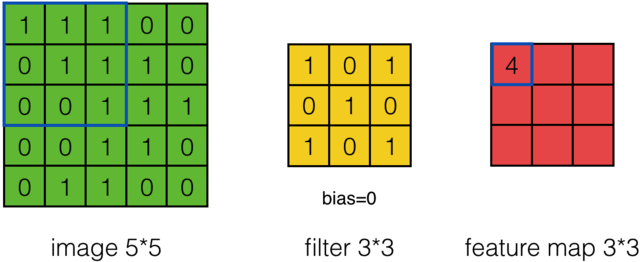
\includegraphics[width=0.8\textwidth]{Cnn5.png}
	\caption{Feature Map}
	\label{fig:Cnn5}
\end{figure}

接下来,Feature Map的元素\(a_{0,1}\)的卷积计算方法为:
\begin{align*}
	a_{0,1} & =f(\sum_{m=0}^{2}\sum_{n=0}^{2}w_{m,n}x_{m+0,n+1}+w_b)                           \\
	        & =relu(w_{0,0}x_{0,1}+w_{0,1}x_{0,2}+w_{0,2}x_{0,3}+w_{1,0}x_{1,1}+w_{1,1}x_{1,2} \\
	        & +w_{1,2}x_{1,3}+w_{2,0}x_{2,1}+w_{2,1}x_{2,3}+w_{2,2}x_{2,3}+w_b)                \\
	        & =relu(1+0+0+0+1+0+0+0+1+0)                                                       \\
	        & =relu(3)=3
\end{align*}


计算结果如图\ref{fig:Cnn6}所示:

\begin{figure}[h]
	\centering
	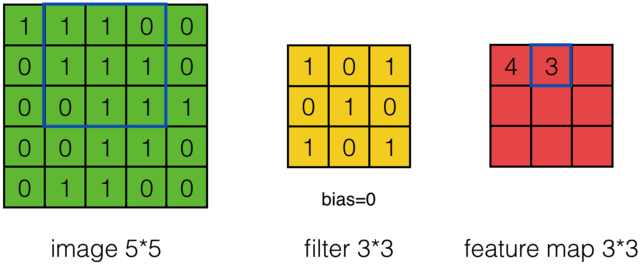
\includegraphics[width=0.8\textwidth]{Cnn6.png}
	\caption{Feature Map}
	\label{fig:Cnn6}
\end{figure}

可以依次计算出Feature Map中所有元素的值。图\ref{fig:Cnn7}显示了整个Feature Map的计算过程:

\begin{figure}[h]
	\centering
	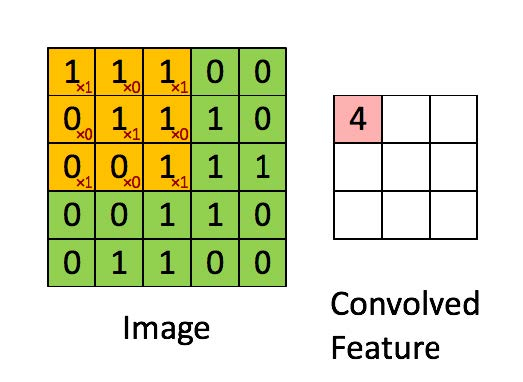
\includegraphics[width=0.6\textwidth]{Cnn7.jpg}
	\caption{Feature Map}
	\label{fig:Cnn7}
\end{figure}

上面的计算过程中,步幅(stride)为1。步幅可以设为大于1的数。例如,当步幅为2时,Feature Map计算如图\ref{fig:Cnn8}。


\begin{figure}[!h]
	\centering
	\subfigure{
		\begin{minipage}[t]{0.7\linewidth}
			\centering
			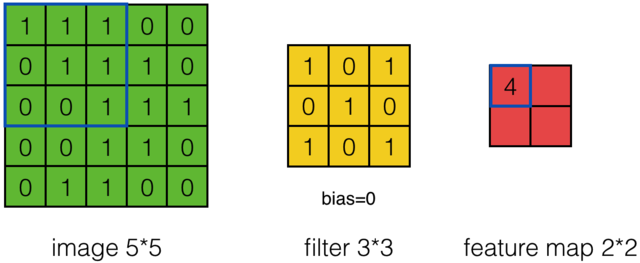
\includegraphics[width=4in]{Cnn8.png}
			%\caption{fig1}
		\end{minipage}%
	}%

	\subfigure{
		\begin{minipage}[t]{0.7\linewidth}
			\centering
			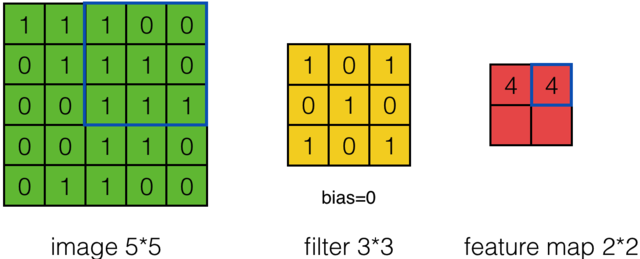
\includegraphics[width=4in]{Cnn9.png}
			%\caption{fig2}
		\end{minipage}%
	}%

	\subfigure{
		\begin{minipage}[t]{0.7\linewidth}
			\centering
			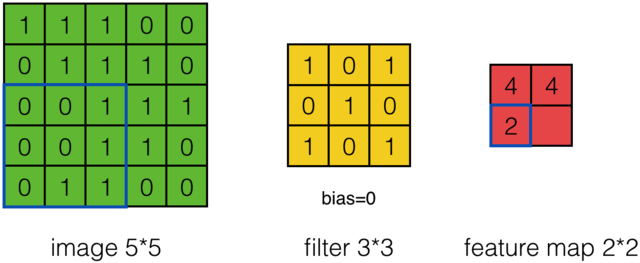
\includegraphics[width=4in]{Cnn10.png}
			%\caption{fig2}
		\end{minipage}%
	}%

	\subfigure{
		\begin{minipage}[t]{0.7\linewidth}
			\centering
			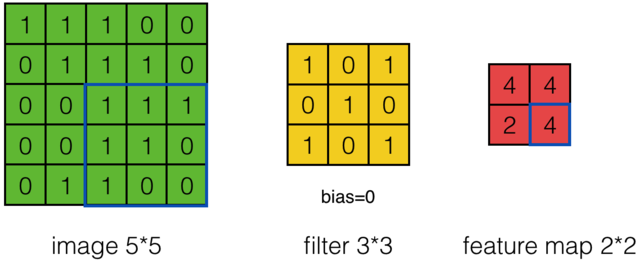
\includegraphics[width=4in]{Cnn11.png}
			%\caption{fig2}
		\end{minipage}%
	}%
	\centering
	\caption{Feature Map计算过程}
	\label{fig:Cnn8}
\end{figure}



我们注意到,当\textbf{步幅}设置为2的时候,Feature Map就变成2*2了。这说明图像大小、步幅和卷积后的Feature Map大小是有关系的。事实上,它们满足下面的关系:
\begin{align}
	W_2 & = (W_1 - F + 2P)/S + 1\label{eq:Cnn2} \\
	H_2 & = (H_1 - F + 2P)/S + 1\label{eq:Cnn3}
\end{align}


在上面两个公式中,\(W_2\)是卷积后Feature Map的宽度;\(W_1\)是卷积前图像的宽度;\(F\)是filter的宽度;\(P\)是\textbf{Zero Padding}数量,\textbf{Zero Padding}是指在原始图像周围补几圈0,如果\(P\)的值是1,那么就补1圈0;\(S\)是\textbf{步幅};\(H_2\)是卷积后Feature Map的高度;\(H_1\)是卷积前图像的宽度。公式\ref{eq:Cnn2}和\ref{eq:Cnn3}本质上是一样的。

以前面的例子来说,图像宽度\(W_1=5\),filter宽度\(F=3\),\textbf{Zero Padding} \(P=0\),\textbf{步幅}\(S=2\),则
\begin{align*}
	W_2 = (W_1 - F + 2P)/S + 1= (5 - 3 + 0)/2 + 1=2
\end{align*}
说明Feature Map宽度是2。同样,我们也可以计算出Feature Map高度也是2。

前面我们已经讲了深度为1的卷积层的计算方法,如果深度大于1怎么计算呢?其实也是类似的。如果卷积前的图像深度为D,那么相应的filter的深度也必须为D。我们扩展一下公式\ref{eq:Cnn1},得到了深度大于1的卷积计算公式:
\begin{equation}
	\label{eq:Cnn4}
	a_{i,j}=f(\sum_{d=0}^{D-1}\sum_{m=0}^{F-1}\sum_{n=0}^{F-1}w_{d,m,n}x_{d,i+m,j+n}+w_b)
\end{equation}


在公式\ref{eq:Cnn4}中,D是深度;F是filter的大小(宽度或高度,两者相同);\(w_{d,m,n}\)表示filter的第\(d\)层第\(m\)行第\(n\)列权重;\(a_{d,i,j}\)表示图像的第\(d\)层第\(i\)行第\(j\)列像素;其它的符号含义和公式\ref{eq:Cnn1}是相同的,不再赘述。

我们前面还曾提到,每个卷积层可以有多个filter。每个filter和原始图像进行卷积后,都可以得到一个Feature Map。因此,卷积后Feature Map的深度(个数)和卷积层的filter个数是相同的。

\begin{figure}[!h]
	\centering
	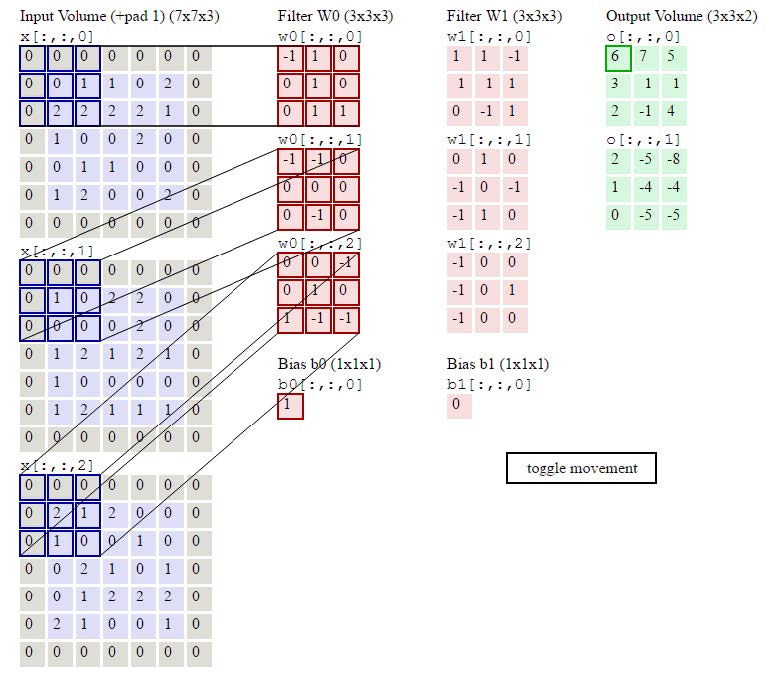
\includegraphics[width=0.9\textwidth]{Cnn12.jpg}
	\caption{卷积过程}
	\label{fig:Cnn12}
\end{figure}

图\ref{fig:Cnn12}显示了包含两个filter的卷积层的计算。我们可以看到7*7*3输入,经过两个3*3*3 filter的卷积(步幅为2),得到了3*3*2的输出。另外我们也会看到下图的\textbf{Zero padding}是1,也就是在输入元素的周围补了一圈0。\textbf{Zero padding}对于图像边缘部分的特征提取是很有帮助的。


以上就是卷积层的计算方法。这里面体现了\textbf{局部连接}和\textbf{权值共享}:每层神经元只和上一层部分神经元相连(卷积计算规则),且filter的权值对于上一层所有神经元都是一样的。对于包含两个3*3*3的fitler的卷积层来说,其参数数量仅有(3*3*3+1)*2=56个,且参数数量与上一层神经元个数无关。与\textbf{全连接神经网络}相比,其参数数量大大减少了。

\textbf{用卷积公式来表达卷积层计算}

不想了解太多数学细节的读者可以跳过这一节,不影响对全文的理解。

公式\ref{eq:Cnn4}的表达很是繁冗,最好能简化一下。就像利用矩阵可以简化表达\textbf{全连接神经网络}的计算一样,我们利用\textbf{卷积公式}可以简化\textbf{卷积神经网络}的表达。

下面我们介绍\textbf{二维卷积公式}。

设矩阵\(A\),\(B\),其行、列数分别为\(m_a\)、\(n_a\)、\(m_b\)、\(n_b\),则\textbf{二维卷积公式}如下:
\begin{align*}
	C_{s,t} & =\sum_0^{m_a-1}\sum_0^{n_a-1} A_{m,n}B_{s-m,t-n}
\end{align*}

且\(s\),\(t\)满足条件$0 \leqslant {s} < {m_a+m_b-1}, 0 \leqslant {t} < {n_a+n_b-1}$。

我们可以把上式写成
\begin{equation}
	\label{eq:Cnn5}
	C = A * B
\end{equation}

如果我们按照公式\ref{eq:Cnn5}来计算卷积,我们可以发现矩阵A实际上是filter,而矩阵B是待卷积的输入,位置关系也有所不同如图\ref{fig:Cnn13}:
\begin{figure}[htbp]
	\centering
	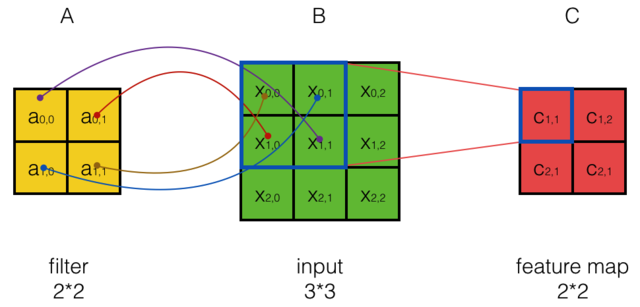
\includegraphics[width=0.7\textwidth]{Cnn13.png}
	\caption{位置关系图}
	\label{fig:Cnn13}
\end{figure}


从上图可以看到,A左上角的值\(a_{0,0}\)与B对应区块中右下角的值\(b_{1,1}\)相乘,而不是与左上角的\(b_{0,0}\)相乘。因此,\textbf{数学}中的卷积和\textbf{卷积神经网络}中的『卷积』还是有区别的,为了避免混淆,我们把\textbf{卷积神经网络}中的『卷积』操作叫做\textbf{互相关(cross-correlation)}操作。

\textbf{卷积}和\textbf{互相关}操作是可以转化的。首先,我们把矩阵A翻转180度,然后再交换A和B的位置(即把B放在左边而把A放在右边。卷积满足交换率,这个操作不会导致结果变化),那么\textbf{卷积}就变成了\textbf{互相关}。

如果我们不去考虑两者这么一点点的区别,我们可以把公式\ref{eq:Cnn5}代入到公式\ref{eq:Cnn4}:
\begin{equation}
	\label{eq:Cnn6}
	A=f(\sum_{d=0}^{D-1}X_d*W_d+w_b)
\end{equation}
其中,\(A\)是卷积层输出的feature map。同公式\ref{eq:Cnn4}相比,公式\ref{eq:Cnn6}就简单多了。然而,这种简洁写法只适合步长为1的情况。


\subsection{Pooling层输出值的计算}\label{Cnn:6}

Pooling层主要的作用是\textbf{下采样},通过去掉Feature Map中不重要的样本,进一步减少参数数量。Pooling的方法很多,最常用的是\textbf{Max Pooling}。\textbf{Max Pooling}实际上就是在n*n的样本中取最大值,作为采样后的样本值。图\ref{fig:Cnn14}是2*2 max pooling。

\begin{figure}[htbp]
	\centering
	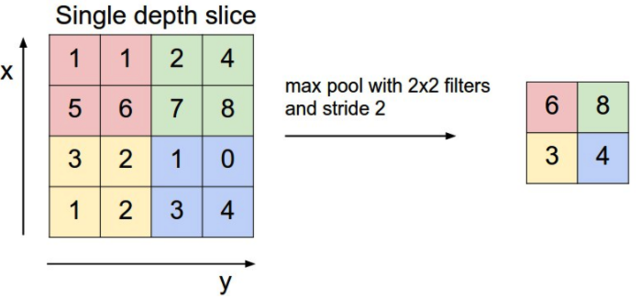
\includegraphics[width=0.7\textwidth]{Cnn14.png}
	\caption{max pooling}
	\label{fig:Cnn14}
\end{figure}

除了\textbf{Max Pooing}之外,常用的还有\textbf{Mean Pooling}---取各样本的平均值。

对于深度为D的Feature Map,各层独立做Pooling,因此Pooling后的深度仍然为D。


\subsection{全连接层}

全连接层输出值的计算和第\ref{chap:Bp}章\textbf{神经网络和反向传播算法}讲过的\textbf{全连接神经网络}是一样的,这里就不再赘述了。

\section{卷积神经网络的训练}\label{Cnn:7}

和\textbf{全连接神经网络}相比,\textbf{卷积神经网络}的训练要复杂一些。但训练的原理是一样的:利用链式求导计算损失函数对每个权重的偏导数(梯度),然后根据梯度下降公式更新权重。训练算法依然是反向传播算法。

我们先回忆一下第\ref{chap:Bp}章\textbf{神经网络和反向传播算法}介绍的反向传播算法,整个算法分为三个步骤:

\begin{enumerate}
	\item
	      前向计算每个神经元的\textbf{输出值}\(a_j\)(\(j\)表示网络的第\(j\)个神经元,以下同);
	\item
	      反向计算每个神经元的\textbf{误差项}\(\delta_j\),\(\delta_j\)在有的文献中也叫做\textbf{敏感度}(sensitivity)。它实际上是网络的损失函数\(E_d\)对神经元\textbf{加权输入}\(net_j\)的偏导数,即\(\delta_j=\frac{\partial{E_d}}{\partial{net_j}}\);
	\item
	      计算每个神经元连接权重\(w_{ji}\)的\textbf{梯度}(\(w_{ji}\)表示从神经元\(i\)连接到神经元\(j\)的权重),公式为\(\frac{\partial{E_d}}{\partial{w_{ji}}}=a_i\delta_j\),其中,\(a_i\)表示神经元\(i\)的输出。
\end{enumerate}

最后,根据梯度下降法则更新每个权重即可。

对于卷积神经网络,由于涉及到\textbf{局部连接}、\textbf{下采样}的等操作,影响到了第二步\textbf{误差项}\(\delta\)的具体计算方法,而\textbf{权值共享}影响了第三步\textbf{权重}\(w\)的\textbf{梯度}的计算方法。接下来,我们分别介绍卷积层和Pooling层的训练算法。

\subsection{卷积层的训练}\label{Cnn:8}

对于卷积层,我们先来看看上面的第二步,即如何将\textbf{误差项}\(\delta\)传递到上一层;然后再来看看第三步,即如何计算filter每个权值\(w\)的\textbf{梯度}。

\textbf{卷积层误差项的传递}

\textbf{最简单情况下误差项的传递}

我们先来考虑步长为1、输入的深度为1、filter个数为1的最简单的情况。

\begin{figure}[!h]
	\centering
	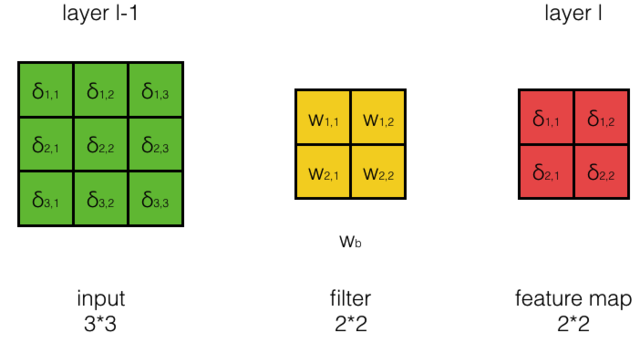
\includegraphics[width=0.7\textwidth]{Cnn15.png}
	\caption{feature map}
	\label{fig:Cnn15}
\end{figure}

假设输入的大小为3*3,filter大小为2*2,按步长为1卷积,我们将得到2*2的\textbf{feature map}。在图\ref{fig:Cnn15}中,为了描述方便,我们为每个元素都进行了编号。用\(\delta^{l-1}_{i,j}\)表示第\(l-1\)层第\(j\)行第\(j\)列的\textbf{误差项};用\(w_{m,n}\)表示filter第\(m\)行第\(n\)列权重,用\(w_b\)表示filter的\textbf{偏置项};用\(a^{l-1}_{i,j}\)表示第\(l-1\)层第\(i\)行第\(j\)列神经元的\textbf{输出};用\(net^{l-1}_{i,j}\)表示第\(l-1\)行神经元的\textbf{加权输入};用\(\delta^l_{i,j}\)表示第\(l\)层第\(j\)行第\(j\)列的\textbf{误差项};用\(f^{l-1}\)表示第\(l-1\)层的\textbf{激活函数}。它们之间的关系如下:
\begin{align*}
	net^l         & =conv(W^l, a^{l-1})+w_b   \\
	a^{l-1}_{i,j} & =f^{l-1}(net^{l-1}_{i,j})
\end{align*}
上式中,\(net^l\)、\(W^l\)、\(a^{l-1}\)都是数组,\(W^l\)是由\(w_{m,n}\)组成的数组,\(conv\)表示卷积操作。

在这里,我们假设第\(l\)中的每个\(\delta^l\)值都已经算好,我们要做的是计算第\(l-1\)层每个神经元的\textbf{误差项}\(\delta^{l-1}\)。

根据链式求导法则:
\begin{align*}
	\delta^{l-1}_{i,j}=\frac{\partial{E_d}}{\partial{net^{l-1}_{i,j}}} =\frac{\partial{E_d}}{\partial{a^{l-1}_{i,j}}}\frac{\partial{a^{l-1}_{i,j}}}{\partial{net^{l-1}_{i,j}}}
\end{align*}

我们先求第一项\(\frac{\partial{E_d}}{\partial{a^{l-1}_{i,j}}}\)。我们先来看几个特例,然后从中总结出一般性的规律。

\begin{example}
	计算\(\frac{\partial{E_d}}{\partial{a^{l-1}_{1,1}}}\),\(a^{l-1}_{1,1}\)仅与\(net^l_{1,1}\)的计算有关:
	\begin{equation*}
		net^j_{1,1}=w_{1,1}a^{l-1}_{1,1}+w_{1,2}a^{l-1}_{1,2}+w_{2,1}a^{l-1}_{2,1}+w_{2,2}a^{l-1}_{2,2}+w_b
	\end{equation*}
\end{example}
因此:
\begin{align*}
	\frac{\partial{E_d}}{\partial{a^{l-1}_{1,1}}}=\frac{\partial{E_d}}{\partial{net^{l}_{1,1}}}\frac{\partial{net^{l}_{1,1}}}{\partial{a^{l-1}_{1,1}}}=\delta^l_{1,1}w_{1,1}
\end{align*}

\begin{example}
	计算\(\frac{\partial{E_d}}{\partial{a^{l-1}_{1,2}}}\),\(a^{l-1}_{1,2}\)与\(net^l_{1,1}\)和\(net^l_{1,2}\)的计算都有关:
	\begin{align*}
		net^j_{1,1} & =w_{1,1}a^{l-1}_{1,1}+w_{1,2}a^{l-1}_{1,2}+w_{2,1}a^{l-1}_{2,1}+w_{2,2}a^{l-1}_{2,2}+w_b \\
		net^j_{1,2} & =w_{1,1}a^{l-1}_{1,2}+w_{1,2}a^{l-1}_{1,3}+w_{2,1}a^{l-1}_{2,2}+w_{2,2}a^{l-1}_{2,3}+w_b
	\end{align*}
\end{example}

因此:
\begin{align*}
	\frac{\partial{E_d}}{\partial{a^{l-1}_{1,2}}}=\frac{\partial{E_d}}{\partial{net^{l}_{1,1}}}\frac{\partial{net^{l}_{1,1}}}{\partial{a^{l-1}_{1,2}}}+\frac{\partial{E_d}}{\partial{net^{l}_{1,2}}}\frac{\partial{net^{l}_{1,2}}}{\partial{a^{l-1}_{1,2}}}=\delta^l_{1,1}w_{1,2}+\delta^l_{1,2}w_{1,1}
\end{align*}

\begin{example}
	计算\(\frac{\partial{E_d}}{\partial{a^{l-1}_{2,2}}}\),\(a^{l-1}_{2,2}\)与\(net^l_{1,1}\)、\(net^l_{1,2}\)、\(net^l_{2,1}\)和\(net^l_{2,2}\)的计算都有关:
	\begin{align*}
		net^j_{1,1} & =w_{1,1}a^{l-1}_{1,1}+w_{1,2}a^{l-1}_{1,2}+w_{2,1}a^{l-1}_{2,1}+w_{2,2}a^{l-1}_{2,2}+w_b \\
		net^j_{1,2} & =w_{1,1}a^{l-1}_{1,2}+w_{1,2}a^{l-1}_{1,3}+w_{2,1}a^{l-1}_{2,2}+w_{2,2}a^{l-1}_{2,3}+w_b \\
		net^j_{2,1} & =w_{1,1}a^{l-1}_{2,1}+w_{1,2}a^{l-1}_{2,2}+w_{2,1}a^{l-1}_{3,1}+w_{2,2}a^{l-1}_{3,2}+w_b \\
		net^j_{2,2} & =w_{1,1}a^{l-1}_{2,2}+w_{1,2}a^{l-1}_{2,3}+w_{2,1}a^{l-1}_{3,2}+w_{2,2}a^{l-1}_{3,3}+w_b
	\end{align*}
\end{example}


因此:
\begin{align*}
	\frac{\partial{E_d}}{\partial{a^{l-1}_{2,2}}} & =\frac{\partial{E_d}}{\partial{net^{l}_{1,1}}}\frac{\partial{net^{l}_{1,1}}}{\partial{a^{l-1}_{2,2}}}+\frac{\partial{E_d}}{\partial{net^{l}_{1,2}}}\frac{\partial{net^{l}_{1,2}}}{\partial{a^{l-1}_{2,2}}}+\frac{\partial{E_d}}{\partial{net^{l}_{2,1}}}\frac{\partial{net^{l}_{2,1}}}{\partial{a^{l-1}_{2,2}}}+\frac{\partial{E_d}}{\partial{net^{l}_{2,2}}}\frac{\partial{net^{l}_{2,2}}}{\partial{a^{l-1}_{2,2}}} \\
	                                              & =\delta^l_{1,1}w_{2,2}+\delta^l_{1,2}w_{2,1}+\delta^l_{2,1}w_{1,2}+\delta^l_{2,2}w_{1,1}
\end{align*}

从上面三个例子,我们发挥一下想象力,不难发现,计算\(\frac{\partial{E_d}}{\partial{a^{l-1}}}\),相当于把第\(l\)层的sensitive map周围补一圈0,在与180度翻转后的filter进行\textbf{cross-correlation},就能得到想要结果,如图\ref{fig:Cnn16}所示。

\begin{figure}[!h]
	\centering
	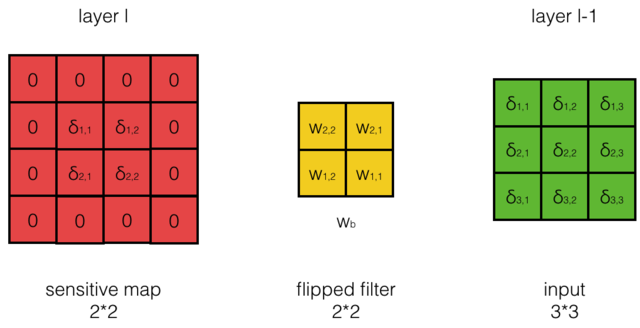
\includegraphics[width=0.7\textwidth]{Cnn16.png}
	\caption{cross correlation}
	\label{fig:Cnn16}
\end{figure}

因为\textbf{卷积}相当于将filter旋转180度的\textbf{cross-correlation},因此上图的计算可以用卷积公式完美的表达:
\[
	\frac{\partial{E_d}}{\partial{a_l}}=\delta^l*W^l
\]

上式中的\(W^l\)表示第\(l\)层的filter的权重数组。也可以把上式的卷积展开,写成求和的形式:
\[
	\frac{\partial{E_d}}{\partial{a^l_{i,j}}}=\sum_m\sum_n{w^l_{m,n}\delta^l_{i+m,j+n}}
\]

现在,我们再求第二项\(\frac{\partial{a^{l-1}_{i,j}}}{\partial{net^{l-1}_{i,j}}}\)。因为
\(
a^{l-1}_{i,j}=f(net^{l-1}_{i,j})
\)
所以这一项极其简单,仅求激活函数\(f\)的导数就行了。
\[
	\frac{\partial{a^{l-1}_{i,j}}}{\partial{net^{l-1}_{i,j}}}=f'(net^{l-1}_{i,j})
\]

将第一项和第二项组合起来,我们得到最终的公式:
\begin{equation}
	\label{eq:Cnn7}
	\delta^{l-1}_{i,j}=\frac{\partial{E_d}}{\partial{net^{l-1}_{i,j}}}=\frac{\partial{E_d}}{\partial{a^{l-1}_{i,j}}}\frac{\partial{a^{l-1}_{i,j}}}{\partial{net^{l-1}_{i,j}}}=\sum_m\sum_n{w^l_{m,n}\delta^l_{i+m,j+n}}f'(net^{l-1}_{i,j})
\end{equation}

也可以将公式\ref{eq:Cnn7}写成卷积的形式:
\begin{equation}
	\label{eq:Cnn8}
	\delta^{l-1}=\delta^l*W^l\circ f'(net^{l-1})\
\end{equation}
其中,符号\(\circ\)表示\textbf{element-wise product},即将矩阵中每个对应元素相乘。注意公式\ref{eq:Cnn8}中的\(\delta^{l-1}\)、\(\delta^l\)、\(net^{l-1}\)都是\textbf{矩阵}。

以上就是步长为1、输入的深度为1、filter个数为1的最简单的情况,卷积层误差项传递的算法。下面我们来推导一下步长为S的情况。

\textbf{卷积步长为S时的误差传递}

我们先来看看步长为S与步长为1的差别。

\begin{figure}[!h]
	\centering
	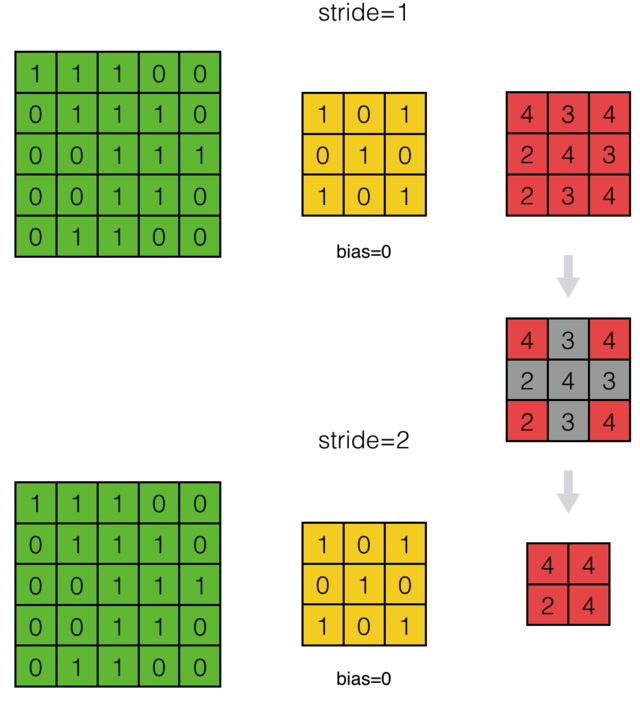
\includegraphics[width=0.75\textwidth]{Cnn17.png}
	\caption{卷积步长的差别}
	\label{fig:Cnn17}
\end{figure}

如图\ref{fig:Cnn17},上面是步长为1时的卷积结果,下面是步长为2时的卷积结果。我们可以看出,因为步长为2,得到的feature map跳过了步长为1时相应的部分。因此,当我们反向计算\textbf{误差项}时,我们可以对步长为S的sensitivity map相应的位置进行补0,将其『还原』成步长为1时的sensitivity map,再用公式\ref{eq:Cnn8}进行求解。

\textbf{输入层深度为D时的误差传递}

当输入深度为D时,filter的深度也必须为D,\(l-1\)层的\(d_i\)通道只与filter的\(d_i\)通道的权重进行计算。因此,反向计算\textbf{误差项}时,我们可以使用\textbf{式8},用filter的第\(d_i\)通道权重对第\(l\)层sensitivity map进行卷积,得到第\(l-1\)层\(d_i\)通道的sensitivity map。如图\ref{fig:Cnn18}所示:

\begin{figure}[!h]
	\centering
	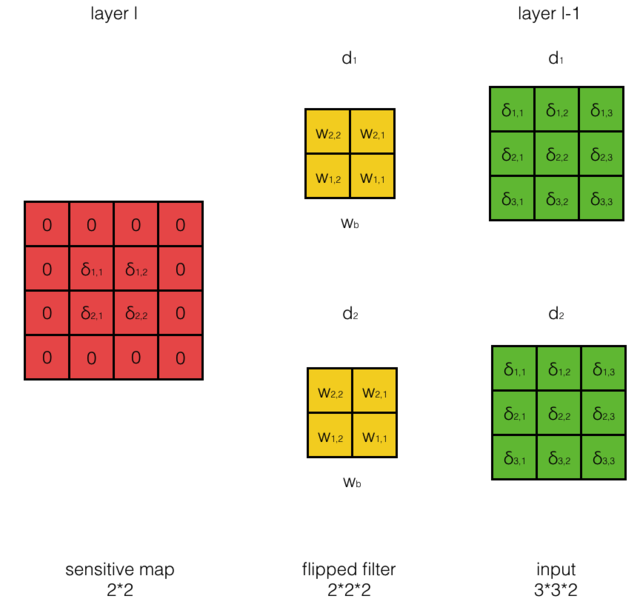
\includegraphics[width=0.8\textwidth]{Cnn18.png}
	\caption{sensitivity map 卷积}
	\label{fig:Cnn18}
\end{figure}

\textbf{filter数量为N时的误差传递}

filter数量为N时,输出层的深度也为N,第\(i\)个filter卷积产生输出层的第\(i\)个feature map。由于第\(l-1\)层\textbf{每个加权输入}\(net^{l-1}_{d, i,j}\)都同时影响了第\(l\)层所有feature map的输出值,因此,反向计算\textbf{误差项}时,需要使用全导数公式。也就是,我们先使用第\(d\)个filter对第\(l\)层相应的第\(d\)个sensitivity map进行卷积,得到一组N个\(l-1\)层的偏sensitivity map。依次用每个filter做这种卷积,就得到D组偏sensitivity map。最后在各组之间将N个偏sensitivity map
\textbf{按元素相加},得到最终的N个\(l-1\)层的sensitivity map:

\begin{equation}
	\label{eq:Cnn9}
	\delta^{l-1}=\sum_{d=0}^D\delta_d^l*W_d^l\circ f'(net^{l-1})
\end{equation}

以上就是卷积层误差项传递的算法,如果读者还有所困惑,可以参考后面的代码实现来理解。

\textbf{卷积层filter权重梯度的计算}

我们要在得到第\(l\)层sensitivity map的情况下,计算filter的权重的梯度,由于卷积层是\textbf{权重共享}的,因此梯度的计算稍有不同。

\begin{figure}[!h]
	\centering
	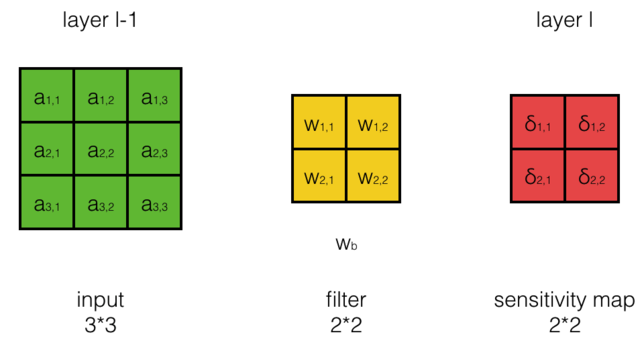
\includegraphics[width=0.8\textwidth]{Cnn19.png}
	\caption{梯度的计算}
	\label{fig:Cnn19}
\end{figure}

如图\ref{fig:Cnn19}所示,\(a^l_{i,j}\)是第\(l-1\)层的输出,\(w_{i,j}\)是第\(l\)层filter的权重,\(\delta^l_{i,j}\)是第\(l\)层的sensitivity map。我们的任务是计算\(w_{i,j}\)的梯度,即\(\frac{\partial{E_d}}{\partial{w_{i,j}}}\)。

为了计算偏导数,我们需要考察权重\(w_{i,j}\)对\(E_d\)的影响。权重项\(w_{i,j}\)通过影响\(net^l_{i,j}\)的值,进而影响\(E_d\)。我们仍然通过几个具体的例子来看权重项\(w_{i,j}\)对\(net^l_{i,j}\)的影响,然后再从中总结出规律。

\begin{example}
	计算\(\frac{\partial{E_d}}{\partial{w_{1,1}}}\):
\end{example}

\begin{align*}
	net^j_{1,1}=w_{1,1}a^{l-1}_{1,1}+w_{1,2}a^{l-1}_{1,2}+w_{2,1}a^{l-1}_{2,1}+w_{2,2}a^{l-1}_{2,2}+w_b \\
	net^j_{1,2}=w_{1,1}a^{l-1}_{1,2}+w_{1,2}a^{l-1}_{1,3}+w_{2,1}a^{l-1}_{2,2}+w_{2,2}a^{l-1}_{2,3}+w_b \\
	net^j_{2,1}=w_{1,1}a^{l-1}_{2,1}+w_{1,2}a^{l-1}_{2,2}+w_{2,1}a^{l-1}_{3,1}+w_{2,2}a^{l-1}_{3,2}+w_b \\
	net^j_{2,2}=w_{1,1}a^{l-1}_{2,2}+w_{1,2}a^{l-1}_{2,3}+w_{2,1}a^{l-1}_{3,2}+w_{2,2}a^{l-1}_{3,3}+w_b
\end{align*}
从上面的公式看出,由于\textbf{权值共享},权值\(w_{1,1}\)对所有的\(net^l_{i,j}\)都有影响。\(E_d\)是\(net^l_{1,1}\)、\(net^l_{1,2}\)、\(net^l_{2,1}\)...的函数,而\(net^l_{1,1}\)、\(net^l_{1,2}\)、\(net^l_{2,1}\)...又是\(w_{1,1}\)的函数,根据\textbf{全导数}公式,计算\(\frac{\partial{E_d}}{\partial{w_{1,1}}}\)就是要把每个偏导数都加起来:
\begin{align*}
	\frac{\partial{E_d}}{\partial{w_{1,1}}} & =\frac{\partial{E_d}}{\partial{net^{l}_{1,1}}}\frac{\partial{net^{l}_{1,1}}}{\partial{w_{1,1}}}+\frac{\partial{E_d}}{\partial{net^{l}_{1,2}}}\frac{\partial{net^{l}_{1,2}}}{\partial{w_{1,1}}}+\frac{\partial{E_d}}{\partial{net^{l}_{2,1}}}\frac{\partial{net^{l}_{2,1}}}{\partial{w_{1,1}}}+\frac{\partial{E_d}}{\partial{net^{l}_{2,2}}}\frac{\partial{net^{l}_{2,2}}}{\partial{w_{1,1}}} \\
	                                        & =\delta^l_{1,1}a^{l-1}_{1,1}+\delta^l_{1,2}a^{l-1}_{1,2}+\delta^l_{2,1}a^{l-1}_{2,1}+\delta^l_{2,2}a^{l-1}_{2,2}
\end{align*}

\begin{example}
	计算\(\frac{\partial{E_d}}{\partial{w_{1,2}}}\):
\end{example}

通过查看\(w_{1,2}\)与\(net^l_{i,j}\)的关系,我们很容易得到:
\[
	\frac{\partial{E_d}}{\partial{w_{1,2}}}=\delta^l_{1,1}a^{l-1}_{1,2}+\delta^l_{1,2}a^{l-1}_{1,3}+\delta^l_{2,1}a^{l-1}_{2,2}+\delta^l_{2,2}a^{l-1}_{2,3}
\]

实际上,每个\textbf{权重项}都是类似的,我们不一一举例了。现在,是我们再次发挥想象力的时候,我们发现计算\(\frac{\partial{E_d}}{\partial{w_{i,j}}}\)规律是:
\[
	\frac{\partial{E_d}}{\partial{w_{i,j}}}=\sum_m\sum_n\delta_{m,n}a^{l-1}_{i+m,j+n}
\]

也就是用sensitivity map作为卷积核,在input上进行\textbf{cross-correlation},如图\ref{fig:Cnn20}所示。

\begin{figure}[h]
	\centering
	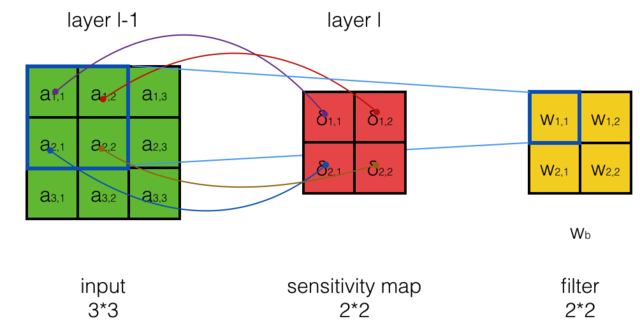
\includegraphics[width=0.7\textwidth]{Cnn20.png}
	\caption{cross correlation}
	\label{fig:Cnn20}
\end{figure}

最后,我们来看一看偏置项的梯度\(\frac{\partial{E_d}}{\partial{w_b}}\)。通过查看前面的公式,我们很容易发现:
\begin{align*}
	\frac{\partial{E_d}}{\partial{w_b}} & =\frac{\partial{E_d}}{\partial{net^{l}_{1,1}}}\frac{\partial{net^{l}_{1,1}}}{\partial{w_b}}+\frac{\partial{E_d}}{\partial{net^{l}_{1,2}}}\frac{\partial{net^{l}_{1,2}}}{\partial{w_b}}+\frac{\partial{E_d}}{\partial{net^{l}_{2,1}}}\frac{\partial{net^{l}_{2,1}}}{\partial{w_b}}+\frac{\partial{E_d}}{\partial{net^{l}_{2,2}}}\frac{\partial{net^{l}_{2,2}}}{\partial{w_b}} \\
	                                    & =\delta^l_{1,1}+\delta^l_{1,2}+\delta^l_{2,1}+\delta^l_{2,2}=\sum_i\sum_j\delta^l_{i,j}
\end{align*}


也就是\textbf{偏置项}的\textbf{梯度}就是sensitivity map所有\textbf{误差项}之和。

对于步长为S的卷积层,处理方法与传递\textbf{误差项}是一样的,首先将sensitivity map『还原』成步长为1时的sensitivity map,再用上面的方法进行计算。

获得了所有的\textbf{梯度}之后,就是根据\textbf{梯度下降算法}来更新每个权重。这在前面的文章中已经反复写过,这里就不再重复了。

至此,我们已经解决了卷积层的训练问题,接下来我们看一看Pooling层的训练。



\subsection{Pooling层的训练}\label{Cnn:9}

无论max pooling还是mean
pooling,都没有需要学习的参数。因此,在\textbf{卷积神经网络}的训练中,Pooling层需要做的仅仅是将\textbf{误差项}传递到上一层,而没有\textbf{梯度}的计算。

\textbf{Max Pooling误差项的传递}

\begin{figure}[!h]
	\centering
	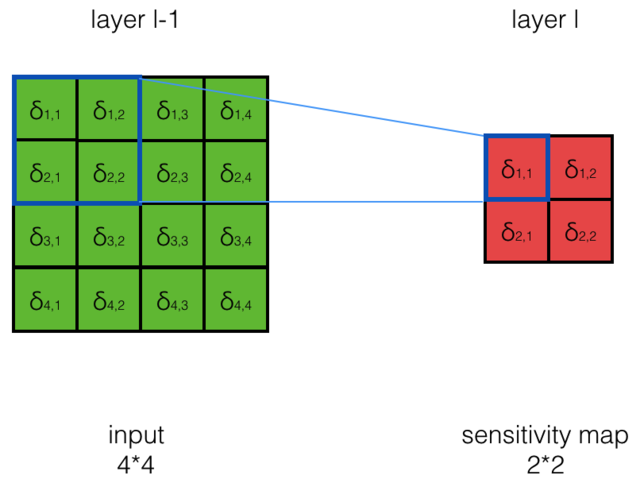
\includegraphics[width=0.6\textwidth]{Cnn21.png}
	\caption{cross correlation}
	\label{fig:Cnn21}
\end{figure}

如图\ref{fig:Cnn21},假设第\(l-1\)层大小为4*4,pooling filter大小为2*2,步长为2,这样,max pooling 之后,第\(l\)层大小为2*2。假设第\(l\)层的\(\delta\)值都已经计算完毕,我们现在的任务是计算第\(l-1\)层的\(\delta\)值。


我们用\(net^{l-1}_{i,j}\)表示第\(l-1\)层的\textbf{加权输入};用\(net^l_{i,j}\)表示第\(l\)层的\textbf{加权输入}。我们先来考察一个具体的例子,然后再总结一般性的规律。对于max pooling:
\[
	net^l_{1,1}=max(net^{l-1}_{1,1},net^{l-1}_{1,2},net^{l-1}_{2,1},net^{l-1}_{2,2})
\]
也就是说,只有区块中最大的\(net^{l-1}_{i,j}\)才会对\(net^l_{i,j}\)的值产生影响。我们假设最大的值是\(net^{l-1}_{1,1}\),则上式相当于:
\[
	net^l_{1,1}=net^{l-1}_{1,1}
\]
那么,我们不难求得下面几个偏导数:
\begin{align*}
	\frac{\partial{net^l_{1,1}}}{\partial{net^{l-1}_{1,1}}}=1, \quad \frac{\partial{net^l_{1,1}}}{\partial{net^{l-1}_{1,2}}}=0 \\
	\frac{\partial{net^l_{1,1}}}{\partial{net^{l-1}_{2,1}}}=0, \quad \frac{\partial{net^l_{1,1}}}{\partial{net^{l-1}_{2,2}}}=0
\end{align*}

因此:
\begin{align*}
	\delta^{l-1}_{1,1} & =\frac{\partial{E_d}}{\partial{net^{l-1}_{1,1}}}=\frac{\partial{E_d}}{\partial{net^{l}_{1,1}}}\frac{\partial{net^{l}_{1,1}}}{\partial{net^{l-1}_{1,1}}}=\delta^{l}_{1,1}, \quad \delta^{l-1}_{1,2}=\frac{\partial{E_d}}{\partial{net^{l-1}_{1,2}}}=\frac{\partial{E_d}}{\partial{net^{l}_{1,1}}}\frac{\partial{net^{l}_{1,1}}}{\partial{net^{l-1}_{1,2}}}=0 \\
	\delta^{l-1}_{2,1} & =\frac{\partial{E_d}}{\partial{net^{l-1}_{2,1}}}=\frac{\partial{E_d}}{\partial{net^{l}_{1,1}}}\frac{\partial{net^{l}_{1,1}}}{\partial{net^{l-1}_{2,1}}}=0, \quad \delta^{l-1}_{1,1}=\frac{\partial{E_d}}{\partial{net^{l-1}_{2,2}}}=\frac{\partial{E_d}}{\partial{net^{l}_{1,1}}}\frac{\partial{net^{l}_{1,1}}}{\partial{net^{l-1}_{2,2}}}=0
\end{align*}

现在,我们发现了规律:对于max pooling,下一层的\textbf{误差项}的值会原封不动的传递到上一层对应区块中的最大值所对应的神经元,而其他神经元的\textbf{误差项}的值都是0。如图\ref{fig:Cnn22}所示(假设\(a^{l-1}_{1,1}\)、\(a^{l-1}_{1,4}\)、\(a^{l-1}_{4,1}\)、\(a^{l-1}_{4,4}\)为所在区块中的最大输出值)。

\begin{figure}[!h]
	\centering
	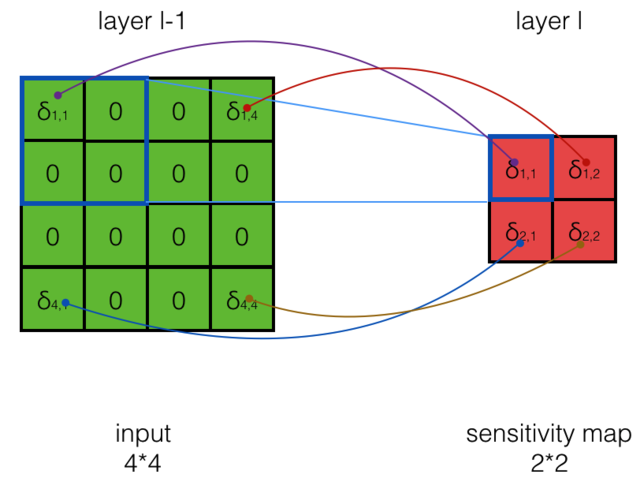
\includegraphics[width=0.6\textwidth]{Cnn22.png}
	\caption{max pooling}
	\label{fig:Cnn22}
\end{figure}

\textbf{Mean Pooling误差项的传递}

我们还是用前面屡试不爽的套路,先研究一个特殊的情形,再扩展为一般规律。
如图\ref{fig:Cnn23},我们先来考虑计算\(\delta^{l-1}_{1,1}\)。我们先来看看\(net^{l-1}_{1,1}\)如何影响\(net^l_{1,1}\)。
\[
	net^j_{1,1}=\frac{1}{4}(net^{l-1}_{1,1}+net^{l-1}_{1,2}+net^{l-1}_{2,1}+net^{l-1}_{2,2})
\]

\begin{figure}[!h]
	\centering
	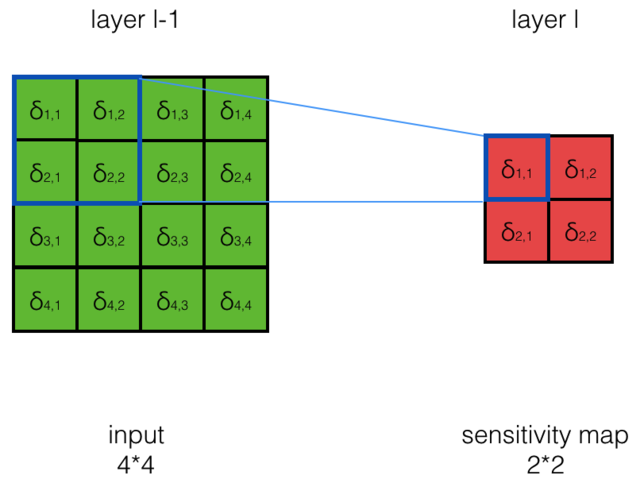
\includegraphics[width=0.6\textwidth]{Cnn23.png}
	\caption{Mean Pooling}
	\label{fig:Cnn23}
\end{figure}
根据上式,我们一眼就能看出来:
\[
	\frac{\partial{net^l_{1,1}}}{\partial{net^{l-1}_{1,1}}}=\frac{1}{4}\\
	\frac{\partial{net^l_{1,1}}}{\partial{net^{l-1}_{1,2}}}=\frac{1}{4}\\
	\frac{\partial{net^l_{1,1}}}{\partial{net^{l-1}_{2,1}}}=\frac{1}{4}\\
	\frac{\partial{net^l_{1,1}}}{\partial{net^{l-1}_{2,2}}}=\frac{1}{4}\\
\]

所以,根据链式求导法则,我们不难算出:
\begin{align*}
	\delta^{l-1}_{1,1} & =\frac{\partial{E_d}}{\partial{net^{l-1}_{1,1}}}=\frac{\partial{E_d}}{\partial{net^{l}_{1,1}}}\frac{\partial{net^{l}_{1,1}}}{\partial{net^{l-1}_{1,1}}}=\frac{1}{4}\delta^{l}_{1,1}, \quad
	\delta^{l-1}_{1,2}=\frac{\partial{E_d}}{\partial{net^{l-1}_{1,2}}}=\frac{\partial{E_d}}{\partial{net^{l}_{1,1}}}\frac{\partial{net^{l}_{1,1}}}{\partial{net^{l-1}_{1,2}}}=\frac{1}{4}\delta^{l}_{1,1}           \\
	\delta^{l-1}_{2,1} & =\frac{\partial{E_d}}{\partial{net^{l-1}_{2,1}}}=\frac{\partial{E_d}}{\partial{net^{l}_{1,1}}}\frac{\partial{net^{l}_{1,1}}}{\partial{net^{l-1}_{2,1}}}=\frac{1}{4}\delta^{l}_{1,1}, \quad
	\delta^{l-1}_{2,2}=\frac{\partial{E_d}}{\partial{net^{l-1}_{2,2}}}=\frac{\partial{E_d}}{\partial{net^{l}_{1,1}}}\frac{\partial{net^{l}_{1,1}}}{\partial{net^{l-1}_{2,2}}}=\frac{1}{4}\delta^{l}_{1,1}
\end{align*}


现在,我们发现了规律:对于mean pooling,下一层的\textbf{误差项}的值会\textbf{平均分配}到上一层对应区块中的所有神经元。如图\ref{fig:Cnn24}所示。
\begin{figure}[!h]
	\centering
	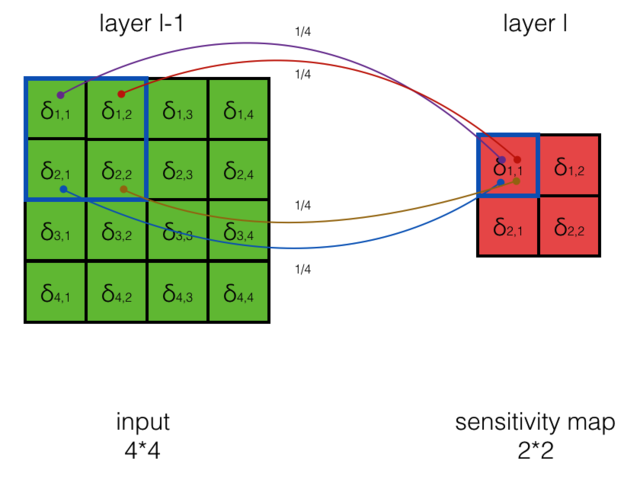
\includegraphics[width=0.6\textwidth]{Cnn24.png}
	\caption{Mean Pooling}
	\label{fig:Cnn24}
\end{figure}

上面这个算法可以表达为高大上的\textbf{克罗内克积(Kronecker product)}的形式,有兴趣的读者可以研究一下。
\[
	\delta^{l-1} = \delta^l\otimes(\frac{1}{n^2})_{n\times n}
\]
其中,\(n\)是pooling层filter的大小,\(\delta^{l-1}\)、\( \delta^l\)都是矩阵。

至此,我们已经把\textbf{卷积层}、\textbf{Pooling层}的训练算法介绍完毕,加上上一篇文章讲的\textbf{全连接层}训练算法,您应该已经具备了编写\textbf{卷积神经网络}代码所需要的知识。为了加深对知识的理解,接下来,我们将展示如何实现一个简单的\textbf{卷积神经网络}。



\section{编程实战:卷积神经网络的实现}\label{Cnn:10}

\begin{note}
	完整代码请参考GitHub: \url{https://github.com/hanbt/learn_dl/blob/master/cnn.py}
	(python2.7)
\end{note}

现在,我们亲自动手实现一个卷积神经网络,以便巩固我们所学的知识。

首先,我们要改变一下代码的架构,『层』成为了我们最核心的组件。这是因为卷积神经网络有不同的层,而每种层的算法都在对应的类中实现。

这次,我们用到了在python中编写算法经常会用到的\textbf{numpy}包。为了使用\textbf{numpy},我们需要先将\textbf{numpy}导入:
\begin{lstlisting}
import numpy as np
\end{lstlisting}

\subsection{卷积层的实现}\label{Cnn:11}

\textbf{卷积层初始化}

我们用\textbf{ConvLayer}类来实现一个卷积层。下面的代码是初始化一个卷积层,可以在构造函数中设置卷积层的\textbf{超参数}。
\begin{lstlisting}
class ConvLayer(object):
    def __init__(self, input_width, input_height, 
                 channel_number, filter_width, 
                 filter_height, filter_number, 
                 zero_padding, stride, activator,
                 learning_rate):
        self.input_width = input_width
        self.input_height = input_height
        self.channel_number = channel_number
        self.filter_width = filter_width
        self.filter_height = filter_height
        self.filter_number = filter_number
        self.zero_padding = zero_padding
        self.stride = stride
        self.output_width = \
            ConvLayer.calculate_output_size(
            self.input_width, filter_width, zero_padding,
            stride)
        self.output_height = \
            ConvLayer.calculate_output_size(
            self.input_height, filter_height, zero_padding,
            stride)
        self.output_array = np.zeros((self.filter_number, 
            self.output_height, self.output_width))
        self.filters = []
        for i in range(filter_number):
            self.filters.append(Filter(filter_width, 
                filter_height, self.channel_number))
        self.activator = activator
        self.learning_rate = learning_rate
\end{lstlisting}

\textbf{calculate\_output\_size}函数用来确定卷积层输出的大小,其实现如下:
\begin{lstlisting}
    @staticmethod
    def calculate_output_size(input_size,
            filter_size, zero_padding, stride):
        return (input_size - filter_size + 
            2 * zero_padding) / stride + 1
\end{lstlisting}

\textbf{Filter}类保存了卷积层的\textbf{参数}以及\textbf{梯度},并且实现了用\textbf{梯度下降算法}来更新参数。
\begin{lstlisting}
class Filter(object):
    def __init__(self, width, height, depth):
        self.weights = np.random.uniform(-1e-4, 1e-4,
            (depth, height, width))
        self.bias = 0
        self.weights_grad = np.zeros(
            self.weights.shape)
        self.bias_grad = 0
    def __repr__(self):
        return 'filter weights:\n%s\nbias:\n%s' % (
            repr(self.weights), repr(self.bias))
    def get_weights(self):
        return self.weights
    def get_bias(self):
        return self.bias
    def update(self, learning_rate):
        self.weights -= learning_rate * self.weights_grad
        self.bias -= learning_rate * self.bias_grad
\end{lstlisting}

我们对参数的初始化采用了常用的策略,即:\textbf{权重}随机初始化为一个很小的值,而\textbf{偏置项}初始化为0。

\textbf{Activator}类实现了\textbf{激活函数},其中,\textbf{forward}方法实现了前向计算,而\textbf{backward}方法则是计算\textbf{导数}。比如,relu函数的实现如下:
\begin{lstlisting}
class ReluActivator(object):
    def forward(self, weighted_input):
        #return weighted_input
        return max(0, weighted_input)
    def backward(self, output):
        return 1 if output > 0 else 0
\end{lstlisting}

\textbf{卷积层前向计算的实现}

\textbf{ConvLayer}类的\textbf{forward}方法实现了卷积层的前向计算(即计算根据输入来计算卷积层的输出),下面是代码实现:
\begin{lstlisting}
    def forward(self, input_array):
        '''
        计算卷积层的输出
        输出结果保存在self.output_array
        '''
        self.input_array = input_array
        self.padded_input_array = padding(input_array,
            self.zero_padding)
        for f in range(self.filter_number):
            filter = self.filters[f]
            conv(self.padded_input_array, 
                filter.get_weights(), self.output_array[f],
                self.stride, filter.get_bias())
        element_wise_op(self.output_array, 
                        self.activator.forward)
\end{lstlisting}

上面的代码里面包含了几个工具函数。\textbf{element\_wise\_op}函数实现了对\textbf{numpy}数组进行\textbf{按元素}操作,并将返回值写回到数组中,代码如下:
\begin{lstlisting}
# 对numpy数组进行element wise操作
def element_wise_op(array, op):
    for i in np.nditer(array,
                       op_flags=['readwrite']):
        i[...] = op(i)
\end{lstlisting}

\textbf{conv}函数实现了2维和3维数组的\textbf{卷积},代码如下:
\begin{lstlisting}
def conv(input_array, 
         kernel_array,
         output_array, 
         stride, bias):
    '''
    计算卷积,自动适配输入为2D和3D的情况
    '''
    channel_number = input_array.ndim
    output_width = output_array.shape[1]
    output_height = output_array.shape[0]
    kernel_width = kernel_array.shape[-1]
    kernel_height = kernel_array.shape[-2]
    for i in range(output_height):
        for j in range(output_width):
            output_array[i][j] = (    
                get_patch(input_array, i, j, kernel_width, 
                    kernel_height, stride) * kernel_array
                ).sum() + bias
\end{lstlisting}

\textbf{padding}函数实现了zero padding操作:
\begin{lstlisting}
# 为数组增加Zero padding
def padding(input_array, zp):
    '''
    为数组增加Zero padding,自动适配输入为2D和3D的情况
    '''
    if zp == 0:
        return input_array
    else:
        if input_array.ndim == 3:
            input_width = input_array.shape[2]
            input_height = input_array.shape[1]
            input_depth = input_array.shape[0]
            padded_array = np.zeros((
                input_depth, 
                input_height + 2 * zp,
                input_width + 2 * zp))
            padded_array[:,
                zp : zp + input_height,
                zp : zp + input_width] = input_array
            return padded_array
        elif input_array.ndim == 2:
            input_width = input_array.shape[1]
            input_height = input_array.shape[0]
            padded_array = np.zeros((
                input_height + 2 * zp,
                input_width + 2 * zp))
            padded_array[zp : zp + input_height,
                zp : zp + input_width] = input_array
            return padded_array
\end{lstlisting}

\textbf{卷积层反向传播算法的实现}

现在,是介绍卷积层核心算法的时候了。我们知道反向传播算法需要完成几个任务:
\begin{enumerate}
	\item
	      将\textbf{误差项}传递到上一层。
	\item
	      计算每个\textbf{参数}的\textbf{梯度}。
	\item
	      更新\textbf{参数}。
\end{enumerate}

以下代码都是在\textbf{ConvLayer}类中实现。我们先来看看将\textbf{误差项}传递到上一层的代码实现。
\begin{lstlisting}
    def bp_sensitivity_map(self, sensitivity_array,
                           activator):
        '''
        计算传递到上一层的sensitivity map
        sensitivity_array: 本层的sensitivity map
        activator: 上一层的激活函数
        '''
        # 处理卷积步长,对原始sensitivity map进行扩展
        expanded_array = self.expand_sensitivity_map(
            sensitivity_array)
        # full卷积,对sensitivitiy map进行zero padding
        # 虽然原始输入的zero padding单元也会获得残差
        # 但这个残差不需要继续向上传递,因此就不计算了
        expanded_width = expanded_array.shape[2]
        zp = (self.input_width +  
              self.filter_width - 1 - expanded_width) / 2
        padded_array = padding(expanded_array, zp)
        # 初始化delta_array,用于保存传递到上一层的
        # sensitivity map
        self.delta_array = self.create_delta_array()
        # 对于具有多个filter的卷积层来说,最终传递到上一层的
        # sensitivity map相当于所有的filter的
        # sensitivity map之和
        for f in range(self.filter_number):
            filter = self.filters[f]
            # 将filter权重翻转180度
            flipped_weights = np.array(map(
                lambda i: np.rot90(i, 2), 
                filter.get_weights()))
            # 计算与一个filter对应的delta_array
            delta_array = self.create_delta_array()
            for d in range(delta_array.shape[0]):
                conv(padded_array[f], flipped_weights[d],
                    delta_array[d], 1, 0)
            self.delta_array += delta_array
        # 将计算结果与激活函数的偏导数做element-wise乘法操作
        derivative_array = np.array(self.input_array)
        element_wise_op(derivative_array, 
                        activator.backward)
        self.delta_array *= derivative_array
\end{lstlisting}

\textbf{expand\_sensitivity\_map}方法就是将步长为S的sensitivity
map『还原』为步长为1的sensitivity map,代码如下:
\begin{lstlisting}
    def expand_sensitivity_map(self, sensitivity_array):
        depth = sensitivity_array.shape[0]
        # 确定扩展后sensitivity map的大小
        # 计算stride为1时sensitivity map的大小
        expanded_width = (self.input_width - 
            self.filter_width + 2 * self.zero_padding + 1)
        expanded_height = (self.input_height - 
            self.filter_height + 2 * self.zero_padding + 1)
        # 构建新的sensitivity_map
        expand_array = np.zeros((depth, expanded_height, 
                                 expanded_width))
        # 从原始sensitivity map拷贝误差值
        for i in range(self.output_height):
            for j in range(self.output_width):
                i_pos = i * self.stride
                j_pos = j * self.stride
                expand_array[:,i_pos,j_pos] = \
                    sensitivity_array[:,i,j]
        return expand_array
\end{lstlisting}

\textbf{create\_delta\_array}是创建用来保存传递到上一层的sensitivity
map的数组。
\begin{lstlisting}
    def create_delta_array(self):
        return np.zeros((self.channel_number,
            self.input_height, self.input_width))
\end{lstlisting}

接下来,是计算梯度的代码。
\begin{lstlisting}
    def bp_gradient(self, sensitivity_array):
        # 处理卷积步长,对原始sensitivity map进行扩展
        expanded_array = self.expand_sensitivity_map(
            sensitivity_array)
        for f in range(self.filter_number):
            # 计算每个权重的梯度
            filter = self.filters[f]
            for d in range(filter.weights.shape[0]):
                conv(self.padded_input_array[d], 
                     expanded_array[f],
                     filter.weights_grad[d], 1, 0)
            # 计算偏置项的梯度
            filter.bias_grad = expanded_array[f].sum()
\end{lstlisting}

最后,是按照\textbf{梯度下降算法}更新参数的代码,这部分非常简单。
\begin{lstlisting}
    def update(self):
        '''
        按照梯度下降,更新权重
        '''
        for filter in self.filters:
            filter.update(self.learning_rate)
\end{lstlisting}

\textbf{卷积层的梯度检查}

为了验证我们的公式推导和代码实现的正确性,我们必须要对卷积层进行梯度检查。下面是代吗实现:
\begin{lstlisting}
def init_test():
    a = np.array(
        [[[0,1,1,0,2],
          [2,2,2,2,1],
          [1,0,0,2,0],
          [0,1,1,0,0],
          [1,2,0,0,2]],
         [[1,0,2,2,0],
          [0,0,0,2,0],
          [1,2,1,2,1],
          [1,0,0,0,0],
          [1,2,1,1,1]],
         [[2,1,2,0,0],
          [1,0,0,1,0],
          [0,2,1,0,1],
          [0,1,2,2,2],
          [2,1,0,0,1]]])
    b = np.array(
        [[[0,1,1],
          [2,2,2],
          [1,0,0]],
         [[1,0,2],
          [0,0,0],
          [1,2,1]]])
    cl = ConvLayer(5,5,3,3,3,2,1,2,IdentityActivator(),0.001)
    cl.filters[0].weights = np.array(
        [[[-1,1,0],
          [0,1,0],
          [0,1,1]],
         [[-1,-1,0],
          [0,0,0],
          [0,-1,0]],
         [[0,0,-1],
          [0,1,0],
          [1,-1,-1]]], dtype=np.float64)
    cl.filters[0].bias=1
    cl.filters[1].weights = np.array(
        [[[1,1,-1],
          [-1,-1,1],
          [0,-1,1]],
         [[0,1,0],
         [-1,0,-1],
          [-1,1,0]],
         [[-1,0,0],
          [-1,0,1],
          [-1,0,0]]], dtype=np.float64)
    return a, b, cl
def gradient_check():
    '''
    梯度检查
    '''
    # 设计一个误差函数,取所有节点输出项之和
    error_function = lambda o: o.sum()
    # 计算forward值
    a, b, cl = init_test()
    cl.forward(a)
    # 求取sensitivity map,是一个全1数组
    sensitivity_array = np.ones(cl.output_array.shape,
                                dtype=np.float64)
    # 计算梯度
    cl.backward(a, sensitivity_array,
                  IdentityActivator())
    # 检查梯度
    epsilon = 10e-4
    for d in range(cl.filters[0].weights_grad.shape[0]):
        for i in range(cl.filters[0].weights_grad.shape[1]):
            for j in range(cl.filters[0].weights_grad.shape[2]):
                cl.filters[0].weights[d,i,j] += epsilon
                cl.forward(a)
                err1 = error_function(cl.output_array)
                cl.filters[0].weights[d,i,j] -= 2*epsilon
                cl.forward(a)
                err2 = error_function(cl.output_array)
                expect_grad = (err1 - err2) / (2 * epsilon)
                cl.filters[0].weights[d,i,j] += epsilon
                print 'weights(%d,%d,%d): expected - actural %f - %f' % (
                    d, i, j, expect_grad, cl.filters[0].weights_grad[d,i,j])   
\end{lstlisting}

上面代码值得思考的地方在于,传递给卷积层的sensitivity
map是全1数组,留给读者自己推导一下为什么是这样(提示:激活函数选择了identity函数:{}\(f(x)=x\))。读者如果还有困惑,请写在文章评论中,我会回复。

运行上面梯度检查的代码,我们得到的输出如下,期望的梯度和实际计算出的梯度一致,这证明我们的算法推导和代码实现确实是正确的。

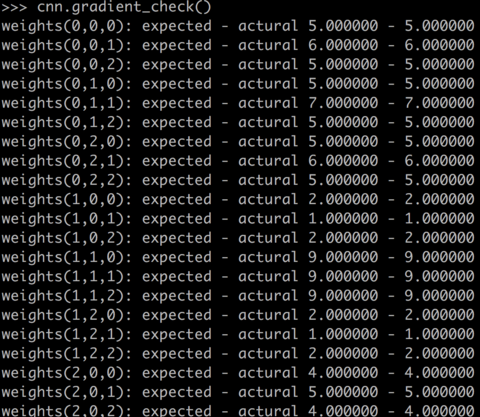
\includegraphics[width=0.7\textwidth]{Cnn25.png}

以上就是卷积层的实现。

\subsection{Max Pooling层的实现}\label{Cnn:12}

max pooling层的实现相对简单,我们直接贴出全部代码如下:
\begin{lstlisting}
class MaxPoolingLayer(object):
    def __init__(self, input_width, input_height, 
                 channel_number, filter_width, 
                 filter_height, stride):
        self.input_width = input_width
        self.input_height = input_height
        self.channel_number = channel_number
        self.filter_width = filter_width
        self.filter_height = filter_height
        self.stride = stride
        self.output_width = (input_width - 
            filter_width) / self.stride + 1
        self.output_height = (input_height -
            filter_height) / self.stride + 1
        self.output_array = np.zeros((self.channel_number,
            self.output_height, self.output_width))
    def forward(self, input_array):
        for d in range(self.channel_number):
            for i in range(self.output_height):
                for j in range(self.output_width):
                    self.output_array[d,i,j] = (    
                        get_patch(input_array[d], i, j,
                            self.filter_width, 
                            self.filter_height, 
                            self.stride).max())
    def backward(self, input_array, sensitivity_array):
        self.delta_array = np.zeros(input_array.shape)
        for d in range(self.channel_number):
            for i in range(self.output_height):
                for j in range(self.output_width):
                    patch_array = get_patch(
                        input_array[d], i, j,
                        self.filter_width, 
                        self.filter_height, 
                        self.stride)
                    k, l = get_max_index(patch_array)
                    self.delta_array[d, 
                        i * self.stride + k, 
                        j * self.stride + l] = \
                        sensitivity_array[d,i,j]
\end{lstlisting}

全连接层的实现和上一篇文章类似,在此就不再赘述了。至此,你已经拥有了实现了一个简单的\textbf{卷积神经网络}所需要的基本组件。对于\textbf{卷积神经网络},现在有很多优秀的开源实现,因此我们并不需要真的自己去实现一个。贴出这些代码的目的是为了让我们更好的了解\textbf{卷积神经网络}的基本原理。



\section{卷积神经网络的应用}\label{Cnn:13}

\textbf{MNIST手写数字识别}

\emph{LeNet-5}是实现手写数字识别的\textbf{卷积神经网络},在MNIST测试集上,它取得了0.8\%的错误率。\emph{LeNet-5}的结构如图\ref{fig:Cnn26}:

\begin{figure}[!h]
	\centering
	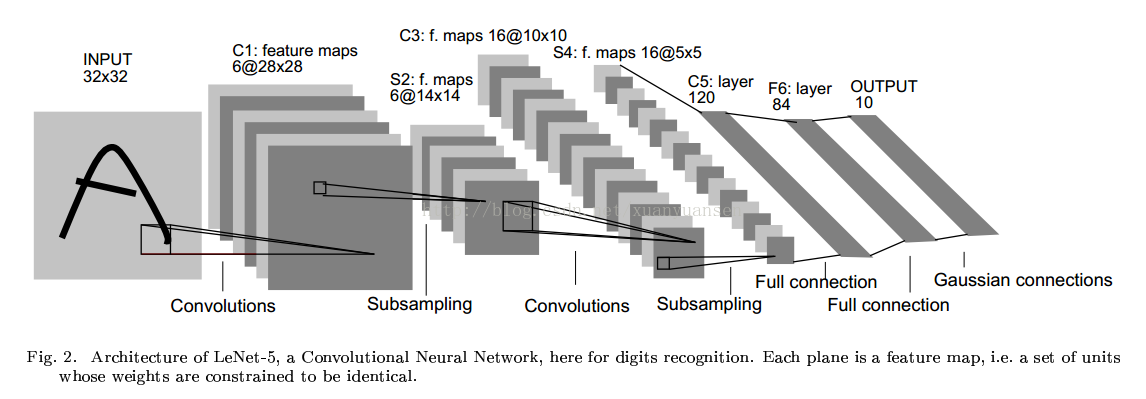
\includegraphics[width=1\textwidth]{Cnn26.png}
	\caption{LeNet-5}
	\label{fig:Cnn26}
\end{figure}

关于\emph{LeNet-5}的详细介绍,网上的资料很多,因此就不再重复了。感兴趣的读者可以尝试用我们自己实现的卷积神经网络代码去构造并训练\emph{LeNet-5}(当然代码会更复杂一些)。

\section{小结}

由于\textbf{卷积神经网络}的复杂性,我们写出了整个系列目前为止最长的一篇文章,相信读者也和作者一样累的要死。\textbf{卷积神经网络}是深度学习最重要的工具(我犹豫要不要写上『之一』呢),付出一些辛苦去理解它也是值得的。如果您真正理解了本文的内容,相当于迈过了入门深度学习最重要的一到门槛。在下一篇文章中,我们介绍深度学习另外一种非常重要的工具:\textbf{循环神经网络},届时我们的系列文章也将完成过半。每篇文章都是一个过滤器,对于坚持到这里的读者们,入门深度学习曙光已现,加油。







\chapter{循环神经网络}\label{chap:Rnn}

\begin{introduction}
	\item 语言模型~\ref{Rnn:1}
	\item 循环神经网络是啥~\ref{Rnn:2}
	\item 基本循环神经网络~\ref{Rnn:3}
	\item 双向循环神经网络~\ref{Rnn:4}
	\item 深度循环神经网络~\ref{Rnn:5}
	\item 循环神经网络的训练~\ref{Rnn:6}
	\item 训练算法:BPTT~\ref{Rnn:7}
	\item 梯度爆炸和消失问题~\ref{Rnn:8}
	\item RNN的应用:语言模型~\ref{Rnn:9}
	\item 向量化~\ref{Rnn:10}
	\item Softmax层~\ref{Rnn:11}
	\item 语言模型的训练~\ref{Rnn:12}
	\item 交叉熵误差~\ref{Rnn:13}
	\item 编程实战:RNN的实现~\ref{Rnn:14}
\end{introduction}


在前面的文章系列文章中,我们介绍了全连接神经网络和卷积神经网络,以及它们的训练和使用。他们都只能单独的取处理一个个的输入,前一个输入和后一个输入是完全没有关系的。但是,某些任务需要能够更好的处理\textbf{序列}的信息,即前面的输入和后面的输入是有关系的。比如,当我们在理解一句话意思时,孤立的理解这句话的每个词是不够的,我们需要处理这些词连接起来的整个\textbf{序列};当我们处理视频的时候,我们也不能只单独的去分析每一帧,而要分析这些帧连接起来的整个\textbf{序列}。这时,就需要用到深度学习领域中另一类非常重要神经网络:\textbf{循环神经网络(Recurrent Neural Network)}。RNN种类很多,也比较绕脑子。不过读者不用担心,本文将一如既往的对复杂的东西剥茧抽丝,帮助您理解RNNs以及它的训练算法,并动手实现一个\textbf{循环神经网络}。


\section{语言模型}\label{Rnn:1}


RNN是在\textbf{自然语言处理}领域中最先被用起来的,比如,RNN可以为\textbf{语言模型}来建模。那么,什么是语言模型呢?

我们可以和电脑玩一个游戏,我们写出一个句子前面的一些词,然后,让电脑帮我们写下接下来的一个词。比如下面这句:
\begin{lstlisting}[numbers=none]
    我昨天上学迟到了,老师批评了 _ _ _ _。
\end{lstlisting}

我们给电脑展示了这句话前面这些词,然后,让电脑写下接下来的一个词。在这个例子中,接下来的这个词最有可能是『我』,而不太可能是『小明』,甚至是『吃饭』。

\textbf{语言模型}就是这样的东西:给定一个一句话前面的部分,预测接下来最有可能的一个词是什么。

\textbf{语言模型}是对一种语言的特征进行建模,它有很多很多用处。比如在语音转文本(STT)的应用中,声学模型输出的结果,往往是若干个可能的候选词,这时候就需要\textbf{语言模型}来从这些候选词中选择一个最可能的。当然,它同样也可以用在图像到文本的识别中(OCR)。

使用RNN之前,语言模型主要是采用N-Gram。N可以是一个自然数,比如2或者3。它的含义是,假设一个词出现的概率只与前面N个词相关。我们以2-Gram为例。首先,对前面的一句话进行切词:
\begin{lstlisting}[numbers=none]
    我 昨天 上学 迟到 了 ,老师 批评 了 _ _ _ _。
\end{lstlisting}


如果用2-Gram进行建模,那么电脑在预测的时候,只会看到前面的『了』,然后,电脑会在语料库中,搜索『了』后面最可能的一个词。不管最后电脑选的是不是『我』,我们都知道这个模型是不靠谱的,因为『了』前面说了那么一大堆实际上是没有用到的。如果是3-Gram模型呢,会搜索『批评了』后面最可能的词,感觉上比2-Gram靠谱了不少,但还是远远不够的。因为这句话最关键的信息『我』,远在9个词之前!

现在读者可能会想,可以提升继续提升N的值呀,比如4-Gram、5-Gram.......。实际上,这个想法是没有实用性的。因为我们想处理任意长度的句子,N设为多少都不合适;另外,模型的大小和N的关系是指数级的,4-Gram模型就会占用海量的存储空间。

所以,该轮到RNN出场了,RNN理论上可以往前看(往后看)任意多个词。

\section{循环神经网络是啥}\label{Rnn:2}

循环神经网络种类繁多,我们先从最简单的基本循环神经网络开始吧。

\subsection{基本循环神经网络}\label{Rnn:3}

图\ref{fig:Rnn1}是一个简单的循环神经网络如,它由输入层、一个隐藏层和一个输出层组成:

\begin{figure}[!h]
	\centering
	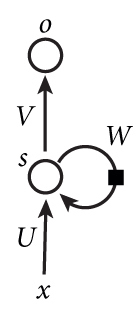
\includegraphics[width=0.15\textwidth]{Rnn1.jpg}
	\caption{简单的循环神经网络}
	\label{fig:Rnn1}
\end{figure}

纳尼?!相信第一次看到这个玩意的读者内心和我一样是崩溃的。因为\textbf{循环神经网络}实在是太难画出来了,网上所有大神们都不得不用了这种抽象艺术手法。不过,静下心来仔细看看的话,其实也是很好理解的。如果把上面有W的那个带箭头的圈去掉,它就变成了最普通的\textbf{全连接神经网络}。$x$是一个向量,它表示\textbf{输入层}的值(这里面没有画出来表示神经元节点的圆圈);$s$是一个向量,它表示\textbf{隐藏层}的值(这里隐藏层面画了一个节点,你也可以想象这一层其实是多个节点,节点数与向量$s$的维度相同);$U$是输入层到隐藏层的\textbf{权重矩阵}(读者可以回到第\ref{chap:Bp}章神经网络和反向传播算法,看看我们是怎样用矩阵来表示\textbf{全连接神经网络}的计算的);$o$也是一个向量,它表示\textbf{输出层}的值;$V$是隐藏层到输出层的\textbf{权重矩阵}。那么,现在我们来看看$W$是什么。\textbf{循环神经网络}的\textbf{隐藏层}的值$s$不仅仅取决于当前这次的输入$x$,还取决于上一次\textbf{隐藏层}的值$s$。\textbf{权重矩阵}
$W$就是\textbf{隐藏层}上一次的值作为这一次的输入的权重。

如果我们把上面的图展开,\textbf{循环神经网络}也可以画成图\ref{fig:Rnn2}这个样子:

\begin{figure}[!h]
	\centering
	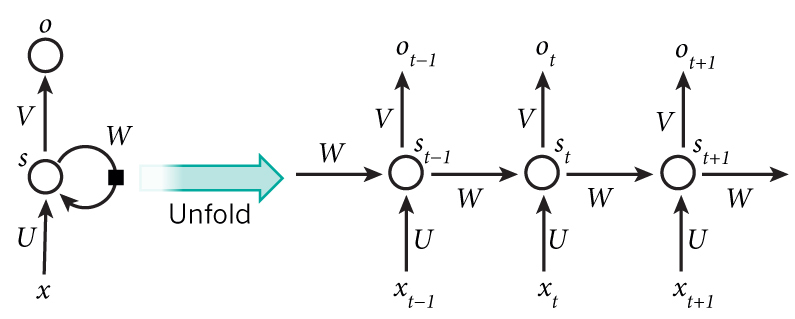
\includegraphics[width=0.8\textwidth]{Rnn2.jpg}
	\caption{循环神经网络}
	\label{fig:Rnn2}
\end{figure}

现在看上去就比较清楚了,这个网络在t时刻接收到输入\({x}_{t}\)之后,隐藏层的值是\({s}_{t}\),输出值是\({o}_{t}\)。关键一点是,\({s}_t\)的值不仅仅取决于\({x}_t\),还取决于\({s}_{t-1}\)。我们可以用下面的公式来表示\textbf{循环神经网络}的计算方法:
\begin{align}
	{o}_t & =g(V{s}_t)\label{eq:Rnn1}            \\
	{s}_t & =f(U{x}_t+W{s}_{t-1})\label{eq:Rnn2}
\end{align}


公式 \ref{eq:Rnn1} 是\textbf{输出层}的计算公式,输出层是一个\textbf{全连接层},也就是它的每个节点都和隐藏层的每个节点相连。$V$是输出层的\textbf{权重矩阵},$g$是\textbf{激活函数}。公式 \ref{eq:Rnn2} 是隐藏层的计算公式,它是\textbf{循环层}。$U$是输入$x$的权重矩阵,$W$是上一次的值\({s}_{t-1}\)作为这一次的输入的\textbf{权重矩阵},$f$是\textbf{激活函数}。

从上面的公式我们可以看出,\textbf{循环层}和\textbf{全连接层}的区别就是\textbf{循环层}多了一个\textbf{权重矩阵}$W$。

如果反复把公式\ref{eq:Rnn2}带入到公式\ref{eq:Rnn1},我们将得到:
\begin{align*}
	{o}_t & =g(V{s}_t)=Vf(U{x}_t+W{s}_{t-1})= g\Big(Vf\big(U{x}_t+Wf(U{x}_{t-1}+W{s}_{t-2})\big)\Big)             \\
	      & = g\Bigg(Vf\Big(U{x}_t+Wf\big(U{x}_{t-1}+Wf(U{x}_{t-2}+W{s}_{t-3})\big)\Big)\Bigg)                    \\
	      & = g\left(Vf\Bigg(U{x}_t+Wf\Big(U{x}_{t-1}+Wf\big(U{x}_{t-2}+Wf(U{x}_{t-3}+...)\big)\Big)\Bigg)\right)
\end{align*}


从上面可以看出,\textbf{循环神经网络}的输出值\(o_t\),是受前面历次输入值\({x}_t\)、\({x}_{t-1}\)、\({x}_{t-2}\)、\({x}_{t-3}\)、...影响的,这就是为什么\textbf{循环神经网络}可以往前看任意多个\textbf{输入值}的原因。




\subsection{双向循环神经网络}\label{Rnn:4}

对于\textbf{语言模型}来说,很多时候光看前面的词是不够的,比如下面这句话:
\begin{lstlisting}[numbers=none]
    我的手机坏了,我打算 _ _ _ _ 一部新手机。
\end{lstlisting}


可以想象,如果我们只看横线前面的词,手机坏了,那么我是打算修一修?换一部新的?还是大哭一场?这些都是无法确定的。但如果我们也看到了横线后面的词是『一部新手机』,那么,横线上的词填『买』的概率就大得多了。

在上一小节中的\textbf{基本循环神经网络}是无法对此进行建模的,因此,我们需要\textbf{双向循环神经网络},如图\ref{fig:Rnn3}所示。

\begin{figure}[!h]
	\centering
	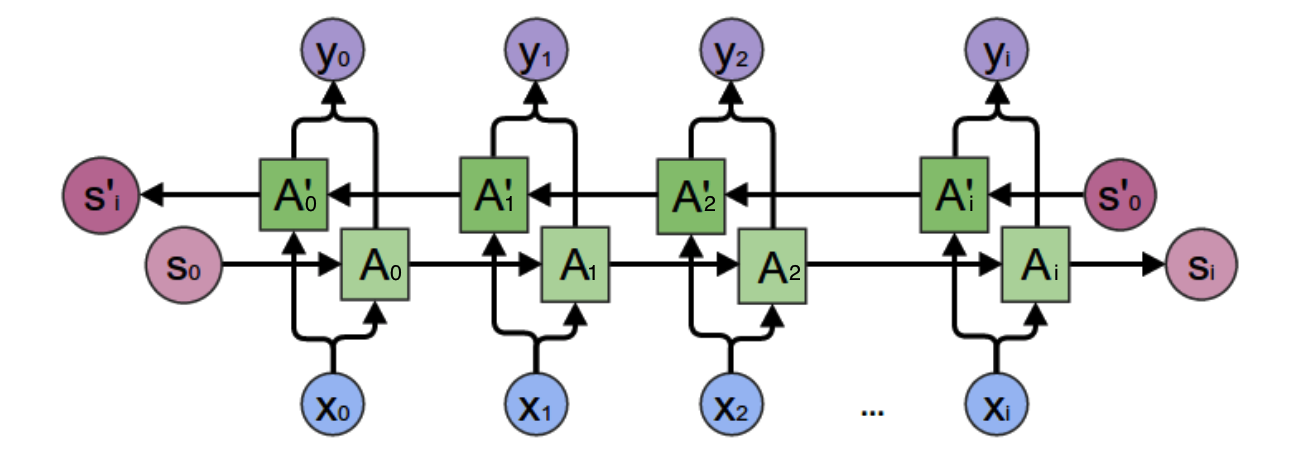
\includegraphics[width=0.8\textwidth]{Rnn3.png}
	\caption{双向循环神经网络}
	\label{fig:Rnn3}
\end{figure}

当遇到这种从未来穿越回来的场景时,难免处于懵逼的状态。不过我们还是可以用屡试不爽的老办法:先分析一个特殊场景,然后再总结一般规律。我们先考虑图\ref{fig:Rnn3}中,\({y}_2\)的计算。

从图\ref{fig:Rnn3}可以看出,\textbf{双向卷积神经网络}的隐藏层要保存两个值,一个$A$参与正向计算,另一个值$A'$参与反向计算。最终的输出值\({y}_2\)取决于\(A_2\)和\(A_2'\)。其计算方法为:
\[
	{y}_2=g(VA_2+V'A_2')
\]

\(A_2\)和\(A_2'\)则分别计算:
\begin{align*}
	A_2  & =f(WA_1+U{x}_2)    \\
	A_2' & =f(W'A_3'+U'{x}_2)
\end{align*}


现在,我们已经可以看出一般的规律:正向计算时,隐藏层的值\({s}_t\)与\({s}_{t-1}\)有关;反向计算时,隐藏层的值\({s}_t'\)与\({s}_{t+1}'\)有关;最终的输出取决于正向和反向计算的\textbf{加和}。现在,我们仿照公式\ref{eq:Rnn1}和\ref{eq:Rnn2},写出双向循环神经网络的计算方法:
\begin{align*}
	{o}_t  & =g(V{s}_t+V'{s}_t')      \\
	{s}_t  & =f(U{x}_t+W{s}_{t-1})    \\
	{s}_t' & =f(U'{x}_t+W'{s}_{t+1}')
\end{align*}


从上面三个公式我们可以看到,正向计算和反向计算\textbf{不共享权重},也就是说$U$和$U'$、$W$和$W'$、$V$和$V'$都是不同的\textbf{权重矩阵}。




\subsection{深度循环神经网络}\label{Rnn:5}
前面我们介绍的\textbf{循环神经网络}只有一个隐藏层,我们当然也可以堆叠两个以上的隐藏层,这样就得到了\textbf{深度循环神经网络}。如图\ref{fig:Rnn4}所示。


我们把第i个隐藏层的值表示为\({s}_t^{(i)}\)、\({s}_t'^{(i)}\),则\textbf{深度循环神经网络}的计算方式可以表示为:
\begin{align*}
	{o}_t        & =g(V^{(i)}{s}_t^{(i)}+V'^{(i)}{s}_t'^{(i)})   \\
	{s}_t^{(i)}  & =f(U^{(i)}{s}_t^{(i-1)}+W^{(i)}{s}_{t-1})     \\
	{s}_t'^{(i)} & =f(U'^{(i)}{s}_t'^{(i-1)}+W'^{(i)}{s}_{t+1}') \\
	...                                                          \\
	{s}_t^{(1)}  & =f(U^{(1)}{x}_t+W^{(1)}{s}_{t-1})             \\
	{s}_t'^{(1)} & =f(U'^{(1)}{x}_t+W'^{(1)}{s}_{t+1}')
\end{align*}


\begin{figure}[!htbp]
	\centering
	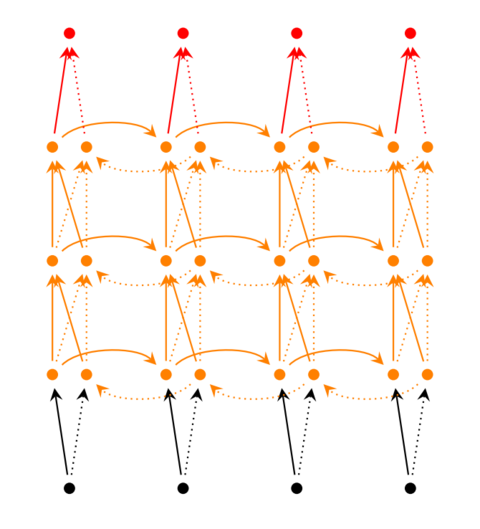
\includegraphics[width=0.4\textwidth]{Rnn4.png}
	\caption{深度循环神经网络}
	\label{fig:Rnn4}
\end{figure}


\section{循环神经网络的训练}\label{Rnn:6}

\subsection{循环神经网络的训练算法:BPTT}\label{Rnn:7}

BPTT算法是针对\textbf{循环层}的训练算法,它的基本原理和BP算法是一样的,也包含同样的三个步骤:

\begin{enumerate}
	\item
	      前向计算每个神经元的输出值;
	\item
	      反向计算每个神经元的\textbf{误差项} \(\delta_j\) 值,它是误差函数$E$对神经元$j$的\textbf{加权输入}\(net_j\)的偏导数;
	\item
	      计算每个权重的梯度。
\end{enumerate}

最后再用\textbf{随机梯度下降}算法更新权重。

循环层如图\ref{fig:Rnn5}所示:

\begin{figure}[!h]
	\centering
	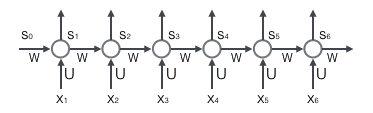
\includegraphics[width=0.6\textwidth]{Rnn5.png}
	\caption{循环层}
	\label{fig:Rnn5}
\end{figure}

\textbf{前向计算}

使用前面的公式\ref{eq:Rnn2}对循环层进行前向计算:
\[
	{s}_t=f(U{x}_t+W{s}_{t-1})
\]

注意,上面的\({s}_t\)、\({x}_t\)、\({s}_{t-1}\)都是向量,用\textbf{黑体字母}表示;而$U$、$V$是\textbf{矩阵},用大写字母表示。\textbf{向量的下标}表示\textbf{时刻},例如,\({s}_t\)表示在$t$时刻向量$s$的值。

我们假设输入向量$x$的维度是$m$,输出向量$s$的维度是$n$,则矩阵$U$的维度是\(n\times m\),矩阵$W$的维度是\(n\times n\)。下面是上式展开成矩阵的样子,看起来更直观一些:
\begin{align*}
	\begin{bmatrix}
		s_1^t  \\
		s_2^t  \\
		\vdots \\
		s_n^t  \\
	\end{bmatrix}=f\left(
	\begin{bmatrix}
		u_{11} u_{12} ... u_{1m} \\
		u_{21} u_{22} ... u_{2m} \\
		\vdots                   \\
		u_{n1} u_{n2} ... u_{nm} \\
	\end{bmatrix}
	\begin{bmatrix}
		x_1^t  \\
		x_2^t  \\
		\vdots \\
		x_m^t  \\
	\end{bmatrix}+
	\begin{bmatrix}
		w_{11} w_{12} ... w_{1n} \\
		w_{21} w_{22} ... w_{2n} \\
		\vdots                   \\
		w_{n1} w_{n2} ... w_{nn} \\
	\end{bmatrix}
	\begin{bmatrix}
		s_1^{t-1} \\
		s_2^{t-1} \\
		\vdots    \\
		s_n^{t-1} \\
	\end{bmatrix}\right)
\end{align*}

在这里我们用\textbf{手写体字母}表示向量的一个\textbf{元素},它的下标表示它是这个向量的第几个元素,它的上标表示第几个\textbf{时刻}。例如,\(s_j^t\)表示向量$s$的第$j$个元素在$t$时刻的值。\(u_{ji}\)表示\textbf{输入层}第$i$个神经元到\textbf{循环层}第$j$个神经元的权重。\(w_{ji}\)表示\textbf{循环层}第$t-1$时刻的第$i$个神经元到\textbf{循环层}第$t$个时刻的第$j$个神经元的权重。

\textbf{误差项的计算}

BTPP算法将第$l$层$t$时刻的\textbf{误差项}\(\delta_t^l\)值沿两个方向传播,一个方向是其传递到上一层网络,得到\(\delta_t^{l-1}\),这部分只和权重矩阵$U$有关;另一个是方向是将其沿时间线传递到初始\(t_1\)时刻,得到\(\delta_1^l\),这部分只和权重矩阵$W$有关。

我们用向量\({net}_t\)表示神经元在$t$时刻的\textbf{加权输入},因为:
\begin{align*}
	{net}_t   & =U{x}_t+W{s}_{t-1} \\
	{s}_{t-1} & =f({net}_{t-1})
\end{align*}


因此:
\begin{align*}
	\frac{\partial{{net}_t}}{\partial{{net}_{t-1}}} & =\frac{\partial{{net}_t}}{\partial{{s}_{t-1}}}\frac{\partial{{s}_{t-1}}}{\partial{{net}_{t-1}}}
\end{align*}


我们用$a$表示列向量,用\({a}^T\)表示行向量。上式的第一项是向量函数对向量求导,其结果为Jacobian矩阵:
\begin{align*}
	\frac{\partial{{net}_t}}{\partial{{s}_{t-1}}} =
	\begin{bmatrix}
		\frac{\partial{net_1^t}}{\partial{s_1^{t-1}}} & \frac{\partial{net_1^t}}{\partial{s_2^{t-1}}} & ... & \frac{\partial{net_1^t}}{\partial{s_n^{t-1}}} \\
		\frac{\partial{net_2^t}}{\partial{s_1^{t-1}}} & \frac{\partial{net_2^t}}{\partial{s_2^{t-1}}} & ... & \frac{\partial{net_2^t}}{\partial{s_n^{t-1}}} \\
		\vdots                                                                                                                                              \\
		\frac{\partial{net_n^t}}{\partial{s_1^{t-1}}} & \frac{\partial{net_n^t}}{\partial{s_2^{t-1}}} & ... & \frac{\partial{net_n^t}}{\partial{s_n^{t-1}}} \\
	\end{bmatrix}
	=\begin{bmatrix}
		w_{11} & w_{12} & ... & w_{1n} \\
		w_{21} & w_{22} & ... & w_{2n} \\
		\vdots                         \\
		w_{n1} & w_{n2} & ... & w_{nn} \\
	\end{bmatrix}=W
\end{align*}


同理,上式第二项也是一个Jacobian矩阵:
\begin{align*}
	\frac{\partial{{s}_{t-1}}}{\partial{{net}_{t-1}}} & =
	\begin{bmatrix}
		\frac{\partial{s_1^{t-1}}}{\partial{net_1^{t-1}}} & \frac{\partial{s_1^{t-1}}}{\partial{net_2^{t-1}}} & ... & \frac{\partial{s_1^{t-1}}}{\partial{net_n^{t-1}}} \\
		\frac{\partial{s_2^{t-1}}}{\partial{net_1^{t-1}}} & \frac{\partial{s_2^{t-1}}}{\partial{net_2^{t-1}}} & ... & \frac{\partial{s_2^{t-1}}}{\partial{net_n^{t-1}}} \\
		\vdots                                                                                                                                                          \\
		\frac{\partial{s_n^{t-1}}}{\partial{net_1^{t-1}}} & \frac{\partial{s_n^{t-1}}}{\partial{net_2^{t-1}}} & ... & \frac{\partial{s_n^{t-1}}}{\partial{net_n^{t-1}}} \\
	\end{bmatrix}                                                      \\
	                                                  & =\begin{bmatrix}
		f'(net_1^{t-1}) & 0               & ... & 0               \\
		0               & f'(net_2^{t-1}) & ... & 0               \\
		\vdots                                                    \\
		0               & 0               & ... & f'(net_n^{t-1}) \\
	\end{bmatrix} \\
	                                                  & =diag[f'({net}_{t-1})]
\end{align*}


其中,$diag({a})$表示根据向量$a$创建一个对角矩阵,即
\[
	diag({a})=\begin{bmatrix}
		a_1 & 0   & ... & 0   \\
		0   & a_2 & ... & 0   \\
		\vdots                \\
		0   & 0   & ... & a_n \\
	\end{bmatrix}
\]

最后,将两项合在一起,可得:
\begin{align*}
	\frac{\partial{{net}_t}}{\partial{{net}_{t-1}}} & =\frac{\partial{{net}_t}}{\partial{{s}_{t-1}}}\frac{\partial{{s}_{t-1}}}{\partial{{net}_{t-1}}}=Wdiag[f'({net}_{t-1})] \\
	                                                & =\begin{bmatrix}
		w_{11}f'(net_1^{t-1}) & w_{12}f'(net_2^{t-1})  & ... & w_{1n}f(net_n^{t-1})   \\
		w_{21}f'(net_1^{t-1}) & w_{22} f'(net_2^{t-1}) & ... & w_{2n}f(net_n^{t-1})   \\
		\vdots                                                                        \\
		w_{n1}f'(net_1^{t-1}) & w_{n2} f'(net_2^{t-1}) & ... & w_{nn} f'(net_n^{t-1}) \\
	\end{bmatrix}
\end{align*}
上式描述了将\(\delta\)沿时间往前传递一个时刻的规律,有了这个规律,我们就可以求得任意时刻$k$的\textbf{误差项}\(\delta_k\):
\begin{align}
	\delta_k^T= & \frac{\partial{E}}{\partial{{net}_k}}=\frac{\partial{E}}{\partial{{net}_t}}\frac{\partial{{net}_t}}{\partial{{net}_k}}=\frac{\partial{E}}{\partial{{net}_t}}\frac{\partial{{net}_t}}{\partial{{net}_{t-1}}}\frac{\partial{{net}_{t-1}}}{\partial{{net}_{t-2}}}...\frac{\partial{{net}_{k+1}}}{\partial{{net}_{k}}}\notag \\
	=           & Wdiag[f'({net}_{t-1})]Wdiag[f'({net}_{t-2})]...Wdiag[f'({net}_{k})]\delta_t^l\notag                                                                                                                                                                                                                                      \\
	=           & \delta_t^T\prod_{i=k}^{t-1}Wdiag[f'({net}_{i})]\label{eq:Rnn3}
\end{align}


公式\ref{eq:Rnn3}就是将误差项沿时间反向传播的算法。

\textbf{循环层}将\textbf{误差项}反向传递到上一层网络,与普通的\textbf{全连接层}是完全一样的,这在第\ref{chap:Bp}章神经网络和反向传播算法中已经详细讲过了,在此仅简要描述一下。

\textbf{循环层}的\textbf{加权输入}\({net}^l\)与上一层的\textbf{加权输入}\({net}^{l-1}\)关系如下:
\begin{align*}
	{net}_t^l=   & U{a}_t^{l-1}+W{s}_{t-1} \\
	{a}_t^{l-1}= & f^{l-1}({net}_t^{l-1})
\end{align*}
上式中\({net}_t^l\)是第$l$层神经元的\textbf{加权输入}(假设第l层是\textbf{循环层});\({net}_t^{l-1}\)是第$l-1$层神经元的\textbf{加权输入};\({a}_t^{l-1}\)是第$l-1$层神经元的输出;\(f^{l-1}\)是第$l-1$层的\textbf{激活函数}。
\[
	\frac{\partial{{net}_t^l}}{\partial{{net}_t^{l-1}}}=\frac{\partial{{net}^l}}{\partial{{a}_t^{l-1}}}\frac{\partial{{a}_t^{l-1}}}{\partial{{net}_t^{l-1}}}=Udiag[f'^{l-1}({net}_t^{l-1})]
\]


所以
\begin{align}
	(\delta_t^{l-1})^T= & \frac{\partial{E}}{\partial{{net}_t^{l-1}}}=\frac{\partial{E}}{\partial{{net}_t^l}}\frac{\partial{{net}_t^l}}{\partial{{net}_t^{l-1}}}\notag \\
	=                   & (\delta_t^l)^TUdiag[f'^{l-1}({net}_t^{l-1})]\label{eq:Rnn4}
\end{align}


公式\ref{eq:Rnn4}就是将误差项传递到上一层算法。

\textbf{权重梯度的计算}

现在,我们终于来到了BPTT算法的最后一步:计算每个权重的梯度。

首先,我们计算误差函数$E$对权重矩阵W的梯度\(\frac{\partial{E}}{\partial{W}}\)。

\begin{figure}[!h]
	\centering
	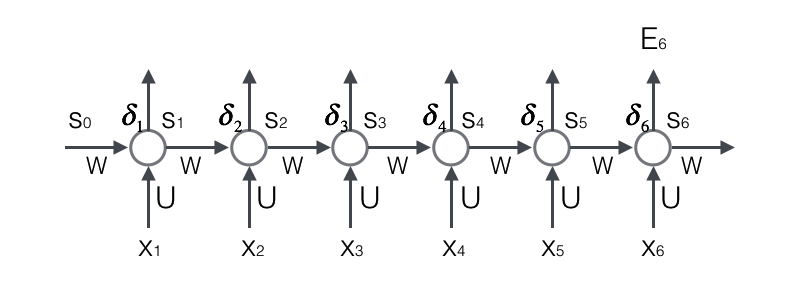
\includegraphics[width=0.8\textwidth]{Rnn6.png}
	\caption{权重梯度}
	\label{fig:Rnn6}
\end{figure}

图\ref{fig:Rnn6}展示了我们到目前为止,在前两步中已经计算得到的量,包括每个时刻t
\textbf{循环层}的输出值\(s_t\),以及误差项\(\delta_t\)。

回忆一下我们在第\ref{chap:Bp}章神经网络和反向传播算法介绍的全连接网络的权重梯度计算算法:只要知道了任意一个时刻的\textbf{误差项}\(\delta_t\),以及上一个时刻循环层的输出值\({s}_{t-1}\),就可以按照下面的公式求出权重矩阵在$t$时刻的梯度\(\nabla_{Wt}E\):
\begin{equation}
	\label{eq:Rnn5}
	\nabla_{W_t}E=\begin{bmatrix}
		\delta_1^ts_1^{t-1} & \delta_1^ts_2^{t-1} & ... & \delta_1^ts_n^{t-1} \\
		\delta_2^ts_1^{t-1} & \delta_2^ts_2^{t-1} & ... & \delta_2^ts_n^{t-1} \\
		\vdots                                                                \\
		\delta_n^ts_1^{t-1} & \delta_n^ts_2^{t-1} & ... & \delta_n^ts_n^{t-1} \\
	\end{bmatrix}
\end{equation}

在公式\ref{eq:Rnn5}中,\(\delta_i^t\)表示t时刻\textbf{误差项}向量的第$i$个分量;\(s_i^{t-1}\)表示$t-1$时刻\textbf{循环层}第$i$个神经元的输出值。

我们下面可以简单推导一下公式\ref{eq:Rnn5}。

我们知道:
\begin{align*}
	{net}_t=                    & U{x}_t+W{s}_{t-1} \\
	\begin{bmatrix}
		net_1^t \\
		net_2^t \\
		\vdots  \\
		net_n^t \\
	\end{bmatrix}= & U{x}_t+
	\begin{bmatrix}
		w_{11} & w_{12} & ... & w_{1n} \\
		w_{21} & w_{22} & ... & w_{2n} \\
		\vdots                         \\
		w_{n1} & w_{n2} & ... & w_{nn} \\
	\end{bmatrix}
	\begin{bmatrix}
		s_1^{t-1} \\
		s_2^{t-1} \\
		\vdots    \\
		s_n^{t-1} \\
	\end{bmatrix}                      \\
	=                           & U{x}_t+
	\begin{bmatrix}
		w_{11}s_1^{t-1}+w_{12}s_2^{t-1} + \cdots + w_{1n}s_n^{t-1} \\
		w_{21}s_1^{t-1}+w_{22}s_2^{t-1} + \cdots + w_{2n}s_n^{t-1} \\
		\vdots                                                     \\
		w_{n1}s_1^{t-1}+w_{n2}s_2^{t-1} + \cdots + w_{nn}s_n^{t-1} \\
	\end{bmatrix}
\end{align*}


因为对$W$求导与\(U{x}_t\)无关,我们不再考虑。现在,我们考虑对权重项\(w_{ji}\)求导。通过观察上式我们可以看到\(w_{ji}\)只与\(net_j^t\)有关,所以:
\[
	\frac{\partial{E}}{\partial{w_{ji}}}=\frac{\partial{E}}{\partial{net_j^t}}\frac{\partial{net_j^t}}{\partial{w_{ji}}}=\delta_j^ts_i^{t-1}
\]


按照上面的规律就可以生成公式\ref{eq:Rnn5}里面的矩阵。

我们已经求得了权重矩阵$W$在$t$时刻的梯度\(\nabla_{Wt}E\),最终的梯度\(\nabla_WE\)是各个时刻的梯度\textbf{之和}:
\begin{align}
	\nabla_WE= & \sum_{i=1}^t\nabla_{W_i}E\notag \\
	=          & \begin{bmatrix}
		\delta_1^ts_1^{t-1} & \delta_1^ts_2^{t-1} & ... & \delta_1^ts_n^{t-1} \\
		\delta_2^ts_1^{t-1} & \delta_2^ts_2^{t-1} & ... & \delta_2^ts_n^{t-1} \\
		\vdots                                                                \\
		\delta_n^ts_1^{t-1} & \delta_n^ts_2^{t-1} & ... & \delta_n^ts_n^{t-1} \\
	\end{bmatrix}+...+
	\begin{bmatrix}
		\delta_1^1s_1^0 & \delta_1^1s_2^0 & ... & \delta_1^1s_n^0 \\
		\delta_2^1s_1^0 & \delta_2^1s_2^0 & ... & \delta_2^1s_n^0 \\
		\vdots                                                    \\
		\delta_n^1s_1^0 & \delta_n^1s_2^0 & ... & \delta_n^1s_n^0 \\
	\end{bmatrix}\label{eq:Rnn6}
\end{align}

公式\ref{eq:Rnn6}就是计算\textbf{循环层}权重矩阵$W$的梯度的公式。

\textbf{——数学公式超高能预警——}

前面已经介绍了\(\nabla_WE\)的计算方法,看上去还是比较直观的。然而,读者也许会困惑,为什么最终的梯度是各个时刻的梯度\textbf{之和}呢?我们前面只是直接用了这个结论,实际上这里面是有道理的,只是这个数学推导比较绕脑子。感兴趣的同学可以仔细阅读接下来这一段,它用到了矩阵对矩阵求导、张量与向量相乘运算的一些法则。

我们还是从这个式子开始:
\[
	{net}_t=U{x}_t+Wf({net}_{t-1})
\]

因为\(U{x}_t\)与$W$完全无关,我们把它看做常量。现在,考虑第一个式子加号右边的部分,因为$W$和\(f({net}_{t-1})\)都是$W$的函数,因此我们要用到大学里面都学过的导数乘法运算:
\[
	(uv)'=u'v+uv'
\]

因此,上面第一个式子写成:
\[
	\frac{\partial{{net}_t}}{\partial{W}}=\frac{\partial{W}}{\partial{W}}f({net}_{t-1})+W\frac{\partial{f({net}_{t-1})}}{\partial{W}}\\
\]

我们最终需要计算的是\(\nabla_WE\):
\begin{align}
	\nabla_WE= & \frac{\partial{E}}{\partial{W}}=\frac{\partial{E}}{\partial{{net}_t}}\frac{\partial{{net}_t}}{\partial{W}}\notag                \\
	=          & \delta_t^T\frac{\partial{W}}{\partial{W}}f({net}_{t-1})+ \delta_t^TW\frac{\partial{f({net}_{t-1})}}{\partial{W}}\label{eq:Rnn7}
\end{align}

我们先计算公式\ref{eq:Rnn7}加号左边的部分。\(\frac{\partial{W}}{\partial{W}}\)是\textbf{矩阵对矩阵求导},其结果是一个四维\textbf{张量(tensor)},如下所示:

\begin{align*}
	\frac{\partial{W}}{\partial{W}}= &
	\begin{bmatrix}
		\frac{\partial{w_{11}}}{\partial{W}} & \frac{\partial{w_{12}}}{\partial{W}} & ... & \frac{\partial{w_{1n}}}{\partial{W}} \\
		\frac{\partial{w_{21}}}{\partial{W}} & \frac{\partial{w_{22}}}{\partial{W}} & ... & \frac{\partial{w_{2n}}}{\partial{W}} \\\vdots \\
		\frac{\partial{w_{n1}}}{\partial{W}} & \frac{\partial{w_{n2}}}{\partial{W}} & ... & \frac{\partial{w_{nn}}}{\partial{W}} \\
	\end{bmatrix}         \\
	=                                &
	\begin{bmatrix}
		\begin{bmatrix}
			\frac{\partial{w_{11}}}{\partial{w_{11}}} & \frac{\partial{w_{11}}}{\partial{w_{12}}} & ... & \frac{\partial{w_{11}}}{\partial{_{1n}}} \\
			\frac{\partial{w_{11}}}{\partial{w_{21}}} & \frac{\partial{w_{11}}}{\partial{w_{22}}} & ... & \frac{\partial{w_{11}}}{\partial{_{2n}}} \\\vdots\\
			\frac{\partial{w_{11}}}{\partial{w_{n1}}} & \frac{\partial{w_{11}}}{\partial{w_{n2}}} & ... & \frac{\partial{w_{11}}}{\partial{_{nn}}} \\
		\end{bmatrix} &
		\begin{bmatrix}
			\frac{\partial{w_{12}}}{\partial{w_{11}}} & \frac{\partial{w_{12}}}{\partial{w_{12}}} & ... & \frac{\partial{w_{12}}}{\partial{_{1n}}} \\
			\frac{\partial{w_{12}}}{\partial{w_{21}}} & \frac{\partial{w_{12}}}{\partial{w_{22}}} & ... & \frac{\partial{w_{12}}}{\partial{_{2n}}} \\\vdots\\
			\frac{\partial{w_{12}}}{\partial{w_{n1}}} & \frac{\partial{w_{12}}}{\partial{w_{n2}}} & ... & \frac{\partial{w_{12}}}{\partial{_{nn}}} \\
		\end{bmatrix} & ... \\\vdots\\
	\end{bmatrix}         \\
	=                                &
	\begin{bmatrix}
		\begin{bmatrix}
			1 & 0 & ... & 0 \\
			0 & 0 & ... & 0 \\
			\vdots          \\
			0 & 0 & ... & 0 \\
		\end{bmatrix} &
		\begin{bmatrix}
			0 & 1 & ... & 0 \\
			0 & 0 & ... & 0 \\
			\vdots          \\
			0 & 0 & ... & 0 \\
		\end{bmatrix} & ... \\
		\vdots                           \\
	\end{bmatrix}
\end{align*}


接下来,我们知道\(s_{t-1}=f({{net}_{t-1}})\),它是一个\textbf{列向量}。我们让上面的四维张量与这个向量相乘,得到了一个三维张量,再左乘行向量\(\delta_t^T\),最终得到一个矩阵:

\begin{align*}
	\delta_t^T\frac{\partial{W}}{\partial{W}}f({{net}_{t-1}})= & \delta_t^T\frac{\partial{W}}{\partial{W}}{{s}_{t-1}}=\delta_t^T
	\begin{bmatrix}
		\begin{bmatrix}
			1 & 0 & ... & 0 \\
			0 & 0 & ... & 0 \\
			\vdots          \\
			0 & 0 & ... & 0 \\
		\end{bmatrix} &
		\begin{bmatrix}
			0 & 1 & ... & 0 \\
			0 & 0 & ... & 0 \\
			\vdots          \\
			0 & 0 & ... & 0 \\
		\end{bmatrix} & ... \\
		\vdots                           \\
	\end{bmatrix}
	\begin{bmatrix}
		s_1^{t-1} \\
		s_2^{t-1} \\
		\vdots    \\
		s_n^{t-1} \\
	\end{bmatrix}                                                                                                   \\
	=                                                          & \delta_t^T
	\begin{bmatrix}
		\begin{bmatrix}
			s_1^{t-1} \\
			0         \\
			\vdots    \\
			0         \\
		\end{bmatrix} &
		\begin{bmatrix}
			s_2^{t-1} \\
			0         \\
			\vdots    \\
			0         \\
		\end{bmatrix} & ... \\
		\vdots                           \\
	\end{bmatrix}=
	\begin{bmatrix}
		\delta_1^t & \delta_2^t & ... & \delta_n^t
	\end{bmatrix}
	\begin{bmatrix}
		\begin{bmatrix}
			s_1^{t-1} \\
			0         \\
			\vdots    \\
			0         \\
		\end{bmatrix} &
		\begin{bmatrix}
			s_2^{t-1} \\
			0         \\
			\vdots    \\
			0         \\
		\end{bmatrix} & ... \\
		\vdots                           \\
	\end{bmatrix}                                                                                                   \\
	=                                                          &
	\begin{bmatrix}
		\delta_1^ts_1^{t-1} & \delta_1^ts_2^{t-1} & ... & \delta_1^ts_n^{t-1} \\
		\delta_2^ts_1^{t-1} & \delta_2^ts_2^{t-1} & ... & \delta_2^ts_n^{t-1} \\
		\vdots                                                                \\
		\delta_n^ts_1^{t-1} & \delta_n^ts_2^{t-1} & ... & \delta_n^ts_n^{t-1} \\
	\end{bmatrix}=\nabla_{Wt}E
\end{align*}


接下来,我们计算公式\ref{eq:Rnn7}加号右边的部分:
\begin{align*}
	\delta_t^TW\frac{\partial{f({net}_{t-1})}}{\partial{W}}= & \delta_t^TW\frac{\partial{f({net}_{t-1})}}{\partial{{net}_{t-1}}}\frac{\partial{{net}_{t-1}}}{\partial{W}}=\delta_t^TWf'({net}_{t-1})\frac{\partial{{net}_{t-1}}}{\partial{W}} \\
	=                                                        & \delta_t^T\frac{\partial{{net}_t}}{\partial{{net}_{t-1}}}\frac{\partial{{net}_{t-1}}}{\partial{W}}=\delta_{t-1}^T\frac{\partial{{net}_{t-1}}}{\partial{W}}
\end{align*}


于是,我们得到了如下递推公式:
\begin{align*}
	\nabla_WE= & \frac{\partial{E}}{\partial{W}}=\frac{\partial{E}}{\partial{{net}_t}}\frac{\partial{{net}_t}}{\partial{W}}=\nabla_{Wt}E+\delta_{t-1}^T\frac{\partial{{net}_{t-1}}}{\partial{W}} \\
	=          & \nabla_{Wt}E+\nabla_{Wt-1}E+\delta_{t-2}^T\frac{\partial{{net}_{t-2}}}{\partial{W}}                                                                                             \\
	=          & \nabla_{Wt}E+\nabla_{Wt-1}E+...+\nabla_{W1}E                                                                                                                                    \\
	=          & \sum_{k=1}^t\nabla_{Wk}E
\end{align*}

这样,我们就证明了:最终的梯度\(\nabla_WE\)是各个时刻的梯度之和。

\textbf{---数学公式超高能预警解除---}

同权重矩阵$W$类似,我们可以得到权重矩阵$U$的计算方法。

\begin{equation}
	\label{eq:Rnn8}
	\nabla_{U_t}E=\begin{bmatrix}
		\delta_1^tx_1^t & \delta_1^tx_2^t & ... & \delta_1^tx_m^t \\
		\delta_2^tx_1^t & \delta_2^tx_2^t & ... & \delta_2^tx_m^t \\
		\vdots                                                    \\
		\delta_n^tx_1^t & \delta_n^tx_2^t & ... & \delta_n^tx_m^t \\
	\end{bmatrix}
\end{equation}

公式\ref{eq:Rnn8}是误差函数在$t$时刻对权重矩阵$U$的梯度。和权重矩阵$W$一样,最终的梯度也是各个时刻的梯度之和:
\[
	\nabla_UE=\sum_{i=1}^t\nabla_{U_i}E
\]

具体的证明这里就不再赘述了,感兴趣的读者可以练习推导一下。

\subsection{RNN的梯度爆炸和消失问题}\label{Rnn:8}

不幸的是,实践中前面介绍的几种RNNs并不能很好的处理较长的序列。一个主要的原因是,RNN在训练中很容易发生\textbf{梯度爆炸}和\textbf{梯度消失},这导致训练时梯度不能在较长序列中一直传递下去,从而使RNN无法捕捉到长距离的影响。

为什么RNN会产生梯度爆炸和消失问题呢?我们接下来将详细分析一下原因。我们根据公式\ref{eq:Rnn3}可得:
\begin{align*}
	\delta_k^T=             & \delta_t^T\prod_{i=k}^{t-1}Wdiag[f'(\mathrm{net}_{i})]             \\
	\|\delta_k^T\|\leqslant & \|\delta_t^T\|\prod_{i=k}^{t-1}\|W\|\|diag[f'(\mathrm{net}_{i})]\| \\
	\leqslant               & \|\delta_t^T\|(\beta_W\beta_f)^{t-k}
\end{align*}

上式的\(\beta\)定义为矩阵的模的上界。因为上式是一个指数函数,如果$t-k$很大的话(也就是向前看很远的时候),会导致对应的\textbf{误差项}的值增长或缩小的非常快,这样就会导致相应的\textbf{梯度爆炸}和\textbf{梯度消失}问题(取决于\(\beta\)大于1还是小于1)。

通常来说,\textbf{梯度爆炸}更容易处理一些。因为梯度爆炸的时候,我们的程序会收到$NaN$错误。我们也可以设置一个梯度阈值,当梯度超过这个阈值的时候可以直接截取。

\textbf{梯度消失}更难检测,而且也更难处理一些。总的来说,我们有三种方法应对梯度消失问题:

\begin{enumerate}
	\item
	      合理的初始化权重值。初始化权重,使每个神经元尽可能不要取极大或极小值,以躲开梯度消失的区域。
	\item
	      使用relu代替sigmoid和tanh作为激活函数。原理请参考第\ref{chap:Cnn}章卷积神经网络的\ref{Cnn:1}\textbf{激活函数}一节。
	\item
	      使用其他结构的RNNs,比如长短时记忆网络(LTSM)和Gated Recurrent   Unit(GRU),这是最流行的做法。我们将在以后的文章中介绍这两种网络。
\end{enumerate}







\section{RNN的应用:基于RNN的语言模型}\label{Rnn:9}

现在,我们介绍一下基于RNN语言模型。我们首先把词依次输入到循环神经网络中,每输入一个词,循环神经网络就输出截止到目前为止,下一个最可能的词。例如,当我们依次输入:
\begin{lstlisting}[numbers=none]
    我 昨天 上学 迟到 了
\end{lstlisting}

神经网络的输出如图\ref{fig:Rnn7}所示:
\begin{figure}[!h]
	\centering
	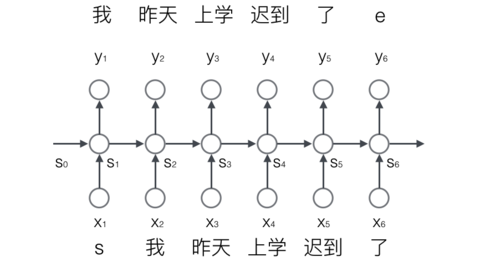
\includegraphics[width=0.7\textwidth]{Rnn7.png}
	\caption{神经网络的输出}
	\label{fig:Rnn7}
\end{figure}

其中,s和e是两个特殊的词,分别表示一个序列的开始和结束。

\subsection{向量化}\label{Rnn:10}

我们知道,神经网络的输入和输出都是\textbf{向量},为了让语言模型能够被神经网络处理,我们必须把词表达为向量的形式,这样神经网络才能处理它。

神经网络的输入是\textbf{词},我们可以用下面的步骤对输入进行\textbf{向量化}:

\begin{enumerate}
	\item
	      建立一个包含所有词的词典,每个词在词典里面有一个唯一的编号。
	\item
	      任意一个词都可以用一个$N$维的one-hot向量来表示。其中,$N$是词典中包含的词的个数。假设一个词在词典中的编号是$i$,$v$是表示这个词的向量,\(v_j\)是向量的第$j$个元素,则:
	      \begin{equation*}
		      v_j=\left\{
		      \begin{aligned}
			      1 & \quad j=i       \\
			      0 & \quad otherwise
		      \end{aligned}
		      \right.
	      \end{equation*}
\end{enumerate}


上面这个公式的含义,可以用图\ref{fig:Rnn8}来直观的表示。
\begin{figure}[!h]
	\centering
	\includegraphics[width=0.9\textwidth]{Rnn8.png}
	\caption{向量化}
	\label{fig:Rnn8}
\end{figure}
使用这种向量化方法,我们就得到了一个高维、\textbf{稀疏}的向量(稀疏是指绝大部分元素的值都是0)。处理这样的向量会导致我们的神经网络有很多的参数,带来庞大的计算量。因此,往往会需要使用一些降维方法,将高维的稀疏向量转变为低维的稠密向量。不过这个话题我们就不再这篇文章中讨论了。

语言模型要求的输出是下一个最可能的词,我们可以让循环神经网络计算计算词典中每个词是下一个词的概率,这样,概率最大的词就是下一个最可能的词。因此,神经网络的输出向量也是一个$N$维向量,向量中的每个元素对应着词典中相应的词是下一个词的概率。如图\ref{fig:Rnn9}所示:

\begin{figure}[!h]
	\centering
	\includegraphics[width=0.9\textwidth]{Rnn9.png}
	\caption{向量化}
	\label{fig:Rnn9}
\end{figure}

\subsection{Softmax层}\label{Rnn:11}

前面提到,\textbf{语言模型}是对下一个词出现的\textbf{概率}进行建模。那么,怎样让神经网络输出概率呢?方法就是用softmax层作为神经网络的输出层。

我们先来看一下softmax函数的定义:
\[
	g(z_i)=\frac{e^{z_i}}{\sum_{k}e^{z_k}}
\]

这个公式看起来可能很晕,我们举一个例子。Softmax层如图\ref{fig:Rnn10}所示,
从图\ref{fig:Rnn10}我们可以看到,softmax layer的输入是一个向量,输出也是一个向量,两个向量的维度是一样的(在这个例子里面是4)。输入向量$x=[1, 2, 3, 4]$经过softmax层之后,经过上面的softmax函数计算,转变为输出向量$y=[0.03, 0.09, 0.24, 0.64]$。计算过程为:
\begin{align*}
	y_1 & =\frac{e^{x_1}}{\sum_{k}e^{x_k}}=\frac{e^1}{e^1+e^2+e^3+e^4}=0.03 \\
	y_2 & =\frac{e^2}{e^1+e^2+e^3+e^4}=0.09                                 \\
	y_3 & =\frac{e^3}{e^1+e^2+e^3+e^4}=0.24                                 \\
	y_4 & =\frac{e^4}{e^1+e^2+e^3+e^4}=0.64
\end{align*}

\begin{figure}[!h]
	\centering
	\includegraphics[width=0.5\textwidth]{Rnn10.png}
	\caption{Softmax层}
	\label{fig:Rnn10}
\end{figure}

我们来看看输出向量$y$的特征:

\begin{enumerate}
	\item
	      每一项为取值为0-1之间的正数;
	\item
	      所有项的总和是1。
\end{enumerate}

我们不难发现,这些特征和\textbf{概率}的特征是一样的,因此我们可以把它们看做是概率。对于\textbf{语言模型}来说,我们可以认为模型预测下一个词是词典中第一个词的概率是0.03,是词典中第二个词的概率是0.09,以此类推。

\subsection{语言模型的训练}\label{Rnn:12}

可以使用\textbf{监督学习}的方法对语言模型进行训练,首先,需要准备训练数据集。接下来,我们介绍怎样把语料
\begin{lstlisting}[numbers=none]
    我 昨天 上学 迟到 了
\end{lstlisting}

转换成语言模型的训练数据集。

首先,我们获取\textbf{输入-标签}对:

\begin{table}[!h]
	\centering
	\setlength{\tabcolsep}{10mm}
	\caption{输入-标签}
	\begin{tabular}{cc}
		\hline
		输入 & 标签 \\ \hline
		s    & 我   \\
		我   & 昨天 \\
		昨天 & 上学 \\
		上学 & 迟到 \\
		迟到 & 了   \\
		了   & e    \\ \hline
	\end{tabular}
\end{table}


然后,使用前面介绍过的\textbf{向量化}方法,对输入$x$和标签$y$进行\textbf{向量化}。这里面有意思的是,对标签$y$进行向量化,其结果也是一个one-hot向量。例如,我们对标签『我』进行向量化,得到的向量中,只有第2019个元素的值是1,其他位置的元素的值都是0。它的含义就是下一个词是『我』的概率是1,是其它词的概率都是0。

最后,我们使用\textbf{交叉熵误差函数}作为优化目标,对模型进行优化。

在实际工程中,我们可以使用大量的语料来对模型进行训练,获取训练数据和训练的方法都是相同的。

\subsection{交叉熵误差}\label{Rnn:13}

一般来说,当神经网络的输出层是softmax层时,对应的误差函数$S$通常选择交叉熵误差函数,其定义如下:
\[
	L(y,o)=-\frac{1}{N}\sum_{n\in{N}}{y_nlogo_n}
\]

在上式中,$N$是训练样本的个数,向量\(y_n\)是样本的标记,向量\(o_n\)是网络的输出。标记\(y_n\)是一个one-hot向量,例如\(y_1=[1,0,0,0]\),如果网络的输出\(o=[0.03,0.09,0.24,0.64]\),那么,交叉熵误差是(假设只有一个训练样本,即N=1):
\begin{align*}
	L & =-\frac{1}{N}\sum_{n\in{N}}{y_nlogo_n}=-y_1logo_1 \\
	  & =-(1*log0.03+0*log0.09+0*log0.24+0*log0.64)=3.51
\end{align*}


我们当然可以选择其他函数作为我们的误差函数,比如最小平方误差函数(MSE)。不过对概率进行建模时,选择交叉熵误差函数更make sense。具体原因,感兴趣的读者请阅读(\url{https://jamesmccaffrey.wordpress.com/2011/12/17/neural-network-classification-categorical-data-softmax-activation-and-cross-entropy-error/})。




\section{编程实战:RNN的实现}\label{Rnn:14}

\begin{note}
	完整代码请参考GitHub: \url{https://github.com/hanbt/learn_dl/blob/master/rnn.py}
	(python2.7)
\end{note}

为了加深我们对前面介绍的知识的理解,我们来动手实现一个RNN层。我们复用了第\ref{chap:Cnn}章卷积神经网络中的一些代码,所以先把它们导入进来。
\begin{lstlisting}
import numpy as np
from cnn import ReluActivator, IdentityActivator, element_wise_op
\end{lstlisting}

我们用RecurrentLayer类来实现一个\textbf{循环层}。下面的代码是初始化一个循环层,可以在构造函数中设置卷积层的超参数。我们注意到,循环层有两个权重数组,U和W。
\begin{lstlisting}
class RecurrentLayer(object):
    def __init__(self, input_width, state_width,
                 activator, learning_rate):
        self.input_width = input_width
        self.state_width = state_width
        self.activator = activator
        self.learning_rate = learning_rate
        self.times = 0       # 当前时刻初始化为t0
        self.state_list = [] # 保存各个时刻的state
        self.state_list.append(np.zeros(
            (state_width, 1)))           # 初始化s0
        self.U = np.random.uniform(-1e-4, 1e-4,
            (state_width, input_width))  # 初始化U
        self.W = np.random.uniform(-1e-4, 1e-4,
            (state_width, state_width))  # 初始化W
\end{lstlisting}

在forward方法中,实现循环层的前向计算,这部分比较简单。
\begin{lstlisting}
    def forward(self, input_array):
        '''
        根据『式2』进行前向计算
        '''
        self.times += 1
        state = (np.dot(self.U, input_array) +
                 np.dot(self.W, self.state_list[-1]))
        element_wise_op(state, self.activator.forward)
        self.state_list.append(state)
\end{lstlisting}

在backword方法中,实现BPTT算法。
\begin{lstlisting}
    def backward(self, sensitivity_array, 
                 activator):
        '''
        实现BPTT算法
        '''
        self.calc_delta(sensitivity_array, activator)
        self.calc_gradient()
    def calc_delta(self, sensitivity_array, activator):
        self.delta_list = []  # 用来保存各个时刻的误差项
        for i in range(self.times):
            self.delta_list.append(np.zeros(
                (self.state_width, 1)))
        self.delta_list.append(sensitivity_array)
        # 迭代计算每个时刻的误差项
        for k in range(self.times - 1, 0, -1):
            self.calc_delta_k(k, activator)
    def calc_delta_k(self, k, activator):
        '''
        根据k+1时刻的delta计算k时刻的delta
        '''
        state = self.state_list[k+1].copy()
        element_wise_op(self.state_list[k+1],
                    activator.backward)
        self.delta_list[k] = np.dot(
            np.dot(self.delta_list[k+1].T, self.W),
            np.diag(state[:,0])).T
    def calc_gradient(self):
        self.gradient_list = [] # 保存各个时刻的权重梯度
        for t in range(self.times + 1):
            self.gradient_list.append(np.zeros(
                (self.state_width, self.state_width)))
        for t in range(self.times, 0, -1):
            self.calc_gradient_t(t)
        # 实际的梯度是各个时刻梯度之和
        self.gradient = reduce(
            lambda a, b: a + b, self.gradient_list,
            self.gradient_list[0]) # [0]被初始化为0且没有被修改过
    def calc_gradient_t(self, t):
        '''
        计算每个时刻t权重的梯度
        '''
        gradient = np.dot(self.delta_list[t],
            self.state_list[t-1].T)
        self.gradient_list[t] = gradient
\end{lstlisting}

有意思的是,BPTT算法虽然数学推导的过程很麻烦,但是写成代码却并不复杂。

在update方法中,实现梯度下降算法。
\begin{lstlisting}
    def update(self):
        '''
        按照梯度下降,更新权重
        '''
        self.W -= self.learning_rate * self.gradient
\end{lstlisting}

上面的代码不包含权重U的更新。这部分实际上和全连接神经网络是一样的,留给感兴趣的读者自己来完成吧。

\textbf{循环层}是一个\textbf{带状态}的层,每次forword都会改变循环层的内部状态,这给梯度检查带来了麻烦。因此,我们需要一个reset\_state方法,来重置循环层的内部状态。
\begin{lstlisting}
    def reset_state(self):
        self.times = 0       # 当前时刻初始化为t0
        self.state_list = [] # 保存各个时刻的state
        self.state_list.append(np.zeros(
            (self.state_width, 1)))      # 初始化s0
\end{lstlisting}

最后,是梯度检查的代码。
\begin{lstlisting}
def gradient_check():
    '''
    梯度检查
    '''
    # 设计一个误差函数,取所有节点输出项之和
    error_function = lambda o: o.sum()
    rl = RecurrentLayer(3, 2, IdentityActivator(), 1e-3)
    # 计算forward值
    x, d = data_set()
    rl.forward(x[0])
    rl.forward(x[1])
    # 求取sensitivity map
    sensitivity_array = np.ones(rl.state_list[-1].shape,
                                dtype=np.float64)
    # 计算梯度
    rl.backward(sensitivity_array, IdentityActivator())
    # 检查梯度
    epsilon = 10e-4
    for i in range(rl.W.shape[0]):
        for j in range(rl.W.shape[1]):
            rl.W[i,j] += epsilon
            rl.reset_state()
            rl.forward(x[0])
            rl.forward(x[1])
            err1 = error_function(rl.state_list[-1])
            rl.W[i,j] -= 2*epsilon
            rl.reset_state()
            rl.forward(x[0])
            rl.forward(x[1])
            err2 = error_function(rl.state_list[-1])
            expect_grad = (err1 - err2) / (2 * epsilon)
            rl.W[i,j] += epsilon
            print 'weights(%d,%d): expected - actural %f - %f' % (
                i, j, expect_grad, rl.gradient[i,j])
\end{lstlisting}

需要注意,每次计算error之前,都要调用reset\_state方法重置循环层的内部状态。下面是梯度检查的结果,没问题!

\includegraphics[width=0.7\textwidth]{Rnn11.png}


\section{小节}

至此,我们讲完了基本的\textbf{循环神经网络}、它的训练算法:\textbf{BPTT},以及在语言模型上的应用。RNN比较烧脑,相信拿下前几篇文章的读者们搞定这篇文章也不在话下吧!然而,\textbf{循环神经网络}这个话题并没有完结。我们在前面说到过,基本的循环神经网络存在梯度爆炸和梯度消失问题,并不能真正的处理好长距离的依赖(虽然有一些技巧可以减轻这些问题)。事实上,真正得到广泛的应用的是循环神经网络的一个变体:\textbf{长短时记忆网络}。它内部有一些特殊的结构,可以很好的处理长距离的依赖,我们将在下一篇文章中详细的介绍它。现在,让我们稍事休息,准备挑战更为烧脑的\textbf{长短时记忆网络}吧。



\chapter{长短时记忆网络}\label{chap:Lstm}

\begin{introduction}
	\item 长短时记忆网络是啥~\ref{Lstm:1}
	\item 长短时记忆网络的前向计算~\ref{Lstm:2}
	\item 长短时记忆网络的训练~\ref{Lstm:3}
	\item LSTM训练算法框架~\ref{Lstm:4}
	\item 关于公式和符号的说明~\ref{Lstm:5}
	\item 误差项沿时间的反向传递~\ref{Lstm:6}
	\item 将误差项传递到上一层~\ref{Lstm:7}
	\item 权重梯度的计算~\ref{Lstm:8}
	\item 编程实战:长短时记忆网络的实现~\ref{Lstm:9}
	\item 激活函数的实现~\ref{Lstm:10}
	\item LSTM初始化~\ref{Lstm:11}
	\item 前向计算的实现~\ref{Lstm:12}
	\item 反向传播算法的实现~\ref{Lstm:13}
	\item 梯度下降算法的实现~\ref{Lstm:14}
	\item 梯度检查的实现~\ref{Lstm:15}
	\item GRU~\ref{Lstm:16}
\end{introduction}

在上一篇文章中,我们介绍了\textbf{循环神经网络}以及它的训练算法。我们也介绍了\textbf{循环神经网络}很难训练的原因,这导致了它在实际应用中,很难处理长距离的依赖。在本文中,我们将介绍一种改进之后的循环神经网络:\textbf{长短时记忆网络(Long Short Term Memory Network, LSTM)},它成功的解决了原始循环神经网络的缺陷,成为当前最流行的RNN,在语音识别、图片描述、自然语言处理等许多领域中成功应用。但不幸的一面是,\textbf{LSTM}的结构很复杂,因此,我们需要花上一些力气,才能把LSTM以及它的训练算法弄明白。在搞清楚\textbf{LSTM}之后,我们再介绍一种\textbf{LSTM}的变体:\textbf{GRU (Gated Recurrent Unit)}。它的结构比\textbf{LSTM}简单,而效果却和\textbf{LSTM}一样好,因此,它正在逐渐流行起来。最后,我们仍然会动手实现一个\textbf{LSTM}。

\section{长短时记忆网络是啥}\label{Lstm:1}

我们首先了解一下长短时记忆网络产生的背景。回顾一下第\ref{chap:Cnn}章循环神经网络中推导的,误差项沿时间反向传播的公式:
\[
	\delta_k^T=\delta_t^T\prod_{i=k}^{t-1}diag[f'({net}_{i})]W
\]

我们可以根据下面的不等式,来获取\(\delta_k^T\)的模的上界(模可以看做对\(\delta_k^T\)中每一项值的大小的度量):
\begin{align*}
	\|\delta_k^T\|\leqslant & \|\delta_t^T\|\prod_{i=k}^{t-1}\|diag[f'({net}_{i})]\|\|W\| \\
	\leqslant               & \|\delta_t^T\|(\beta_f\beta_W)^{t-k}
\end{align*}

我们可以看到,误差项\(\delta\)从t时刻传递到k时刻,其值的上界是\(\beta_f\beta_w\)的指数函数。\(\beta_f\beta_w\)分别是对角矩阵\(diag[f'({net}_{i})]\)和矩阵W模的上界。显然,除非\(\beta_f\beta_w\)乘积的值位于1附近,否则,当t-k很大时(也就是误差传递很多个时刻时),整个式子的值就会变得极小(当\(\beta_f\beta_w\)乘积小于1)或者极大(当\(\beta_f\beta_w\)乘积大于1),前者就是\textbf{梯度消失},后者就是\textbf{梯度爆炸}。虽然科学家们搞出了很多技巧(比如怎样初始化权重),让\(\beta_f\beta_w\)的值尽可能贴近于1,终究还是难以抵挡指数函数的威力。

\textbf{梯度消失}到底意味着什么?在第\ref{chap:Cnn}章循环神经网络中我们已证明,权重数组W最终的梯度是各个时刻的梯度之和,即:
\begin{align*}
	\nabla_WE & =\sum_{k=1}^t\nabla_{Wk}E=\nabla_{Wt}E+\nabla_{Wt-1}E+\nabla_{Wt-2}E+...+\nabla_{W1}E
\end{align*}

假设某轮训练中,各时刻的梯度以及最终的梯度之和如图\ref{fig:Lstm1}:
\begin{figure}[!h]
	\centering
	\includegraphics[width=0.7\textwidth]{Lstm1.png}
	\caption{梯度}
	\label{fig:Lstm1}
\end{figure}
我们就可以看到,从上图的t-3时刻开始,梯度已经几乎减少到0了。那么,从这个时刻开始再往之前走,得到的梯度(几乎为零)就不会对最终的梯度值有任何贡献,这就相当于无论t-3时刻之前的网络状态h是什么,在训练中都不会对权重数组W的更新产生影响,也就是网络事实上已经忽略了t-3时刻之前的状态。这就是原始RNN无法处理长距离依赖的原因。

既然找到了问题的原因,那么我们就能解决它。从问题的定位到解决,科学家们大概花了7、8年时间。终于有一天,Hochreiter和Schmidhuber两位科学家发明出\textbf{长短时记忆网络},一举解决这个问题。

其实,\textbf{长短时记忆网络}的思路比较简单。原始RNN的隐藏层只有一个状态,即h,它对于短期的输入非常敏感。那么,假如我们再增加一个状态,即c,让它来保存长期的状态,那么问题不就解决了么?如图\ref{fig:Lstm2}所示:
\begin{figure}[!h]
	\centering
	\includegraphics[width=0.35\textwidth]{Lstm2.png}
	\caption{RNN to LSTM}
	\label{fig:Lstm2}
\end{figure}

新增加的状态c,称为\textbf{单元状态(cell state)}。我们把上图按照时间维度展开:
\begin{figure}[!h]
	\centering
	\includegraphics[width=0.7\textwidth]{Lstm3.png}
	\caption{梯度}
	\label{fig:Lstm3}
\end{figure}

图\ref{fig:Lstm3}仅仅是一个示意图,我们可以看出,在t时刻,LSTM的输入有三个:当前时刻网络的输入值\({x}_t\)、上一时刻LSTM的输出值\({h}_{t-1}\)、以及上一时刻的单元状态\({c}_{t-1}\);LSTM的输出有两个:当前时刻LSTM输出值\({h}_t\)、和当前时刻的单元状态\({c}_t\)。注意\({x}\)、\({h}\)、\({c}\)都是\textbf{向量}。

LSTM的关键,就是怎样控制长期状态c。在这里,LSTM的思路是使用三个控制开关。第一个开关,负责控制继续保存长期状态c;第二个开关,负责控制把即时状态输入到长期状态c;第三个开关,负责控制是否把长期状态c作为当前的LSTM的输出。三个开关的作用如图\ref{fig:Lstm4}所示:

\begin{figure}[!h]
	\centering
	\includegraphics[width=0.6\textwidth]{Lstm4.png}
	\caption{梯度}
	\label{fig:Lstm4}
\end{figure}


接下来,我们要描述一下,输出h和单元状态c的具体计算方法。

\section{长短时记忆网络的前向计算}\label{Lstm:2}

前面描述的开关是怎样在算法中实现的呢?这就用到了\textbf{门(gate)}的概念。门实际上就是一层\textbf{全连接层},它的输入是一个向量,输出是一个0到1之间的实数向量。假设W是门的权重向量,\({b}\)是偏置项,那么门可以表示为:
\[
	g({x})=\sigma(W{x}+{b})
\]

门的使用,就是用门的输出向量按元素乘以我们需要控制的那个向量。因为门的输出是0到1之间的实数向量,那么,当门输出为0时,任何向量与之相乘都会得到0向量,这就相当于啥都不能通过;输出为1时,任何向量与之相乘都不会有任何改变,这就相当于啥都可以通过。因为\(\sigma\)(也就是sigmoid函数)的值域是(0,1),所以门的状态都是半开半闭的。

LSTM用两个门来控制单元状态c的内容,一个是\textbf{遗忘门(forget gate)},它决定了上一时刻的单元状态\({c}_{t-1}\)有多少保留到当前时刻\({c}_t\);另一个是\textbf{输入门(input gate)},它决定了当前时刻网络的输入\({x}_t\)有多少保存到单元状态\({c}_t\)。LSTM用\textbf{输出门(output gate)}来控制单元状态\({c}_t\)有多少输出到LSTM的当前输出值\({h}_t\)。

我们先来看一下遗忘门:
\begin{equation}
	\label{eq:Lstm1}
	{f}_t=\sigma(W_f\cdot[{h}_{t-1},{x}_t]+{b}_f)
\end{equation}
上式中,\(W_f\)是遗忘门的权重矩阵,\([{h}_{t-1},{x}_t]\)表示把两个向量连接成一个更长的向量,\({b}_f\)是遗忘门的偏置项,\(\sigma\)是sigmoid函数。如果输入的维度是\(d_x\),隐藏层的维度是\(d_h\),单元状态的维度是\(d_c\)(通常\(d_c=d_h\)),则遗忘门的权重矩阵\(W_f\)维度是\( d_c\times (d_h+d_x)\)。事实上,权重矩阵\(W_f\)都是两个矩阵拼接而成的:一个是\(W_{fh}\),它对应着输入项\({h}_{t-1}\),其维度为\(d_c\times d_h\);一个是\(W_{fx}\),它对应着输入项\({x}_t\),其维度为\(d_c\times d_x\)。\(W_f\)可以写为:
\begin{align*}
	\begin{bmatrix}W_f\end{bmatrix}\begin{bmatrix}{h}_{t-1} \\
		{x}_t\end{bmatrix} & =\begin{bmatrix}W_{fh}&W_{fx}\end{bmatrix}\begin{bmatrix}{h}_{t-1} \\
		{x}_t\end{bmatrix} \\
	                                                    & =W_{fh}{h}_{t-1}+W_{fx}{x}_t
\end{align*}

图\ref{fig:Lstm5}显示了遗忘门的计算:
\begin{figure}[!h]
	\centering
	\includegraphics[width=0.6\textwidth]{Lstm5.png}
	\caption{遗忘门}
	\label{fig:Lstm5}
\end{figure}

接下来看看输入门:
\begin{equation}
	\label{eq:Lstm2}
	{i}_t=\sigma(W_i\cdot[{h}_{t-1},{x}_t]+{b}_i)
\end{equation}
上式中,\(W_i\)是输入门的权重矩阵,\({b}_i\)是输入门的偏置项。图\ref{fig:Lstm6}表示了输入门的计算:
\begin{figure}[!h]
	\centering
	\includegraphics[width=0.6\textwidth]{Lstm6.png}
	\caption{输入门}
	\label{fig:Lstm6}
\end{figure}

接下来,我们计算用于描述当前输入的单元状态\({\tilde{c}}_t\),它是根据上一次的输出和本次输入来计算的:
\begin{equation}
	\label{eq:Lstm3}
	{\tilde{c}}_t=\tanh(W_c\cdot[{h}_{t-1},{x}_t]+{b}_c)
\end{equation}

图\ref{fig:Lstm7}是\({\tilde{c}}_t\)的计算:
\begin{figure}[!h]
	\centering
	\includegraphics[width=0.6\textwidth]{Lstm7.png}
	\caption{\({\tilde{c}}_t\)的计算}
	\label{fig:Lstm7}
\end{figure}
现在,我们计算当前时刻的单元状态\({c}_t\)。它是由上一次的单元状态\({c}_{t-1}\)按元素乘以遗忘门\(f_t\),再用当前输入的单元状态\({\tilde{c}}_t\)按元素乘以输入门\(i_t\),再将两个积加和产生的:
\begin{equation}
	\label{eq:Lstm4}
	{c}_t=f_t\circ{{c}_{t-1}}+i_t\circ{{\tilde{c}}_t}
\end{equation}
符号\(\circ\)表示\textbf{按元素乘}。图\ref{fig:Lstm8}是\({c}_t\)的计算:

\begin{figure}[!h]
	\centering
	\includegraphics[width=0.6\textwidth]{Lstm8.png}
	\caption{\({c}_t\)的计算}
	\label{fig:Lstm8}
\end{figure}

这样,我们就把LSTM关于当前的记忆\({\tilde{c}}_t\)和长期的记忆\({c}_{t-1}\)组合在一起,形成了新的单元状态\({c}_t\)。由于遗忘门的控制,它可以保存很久很久之前的信息,由于输入门的控制,它又可以避免当前无关紧要的内容进入记忆。下面,我们要看看输出门,它控制了长期记忆对当前输出的影响:
\begin{equation}
	\label{eq:Lstm5}
	{o}_t=\sigma(W_o\cdot[{h}_{t-1},{x}_t]+{b}_o)
\end{equation}

图\ref{fig:Lstm9}表示输出门的计算:

\begin{figure}[!h]
	\centering
	\includegraphics[width=0.6\textwidth]{Lstm9.png}
	\caption{输出门}
	\label{fig:Lstm9}
\end{figure}

LSTM最终的输出,是由输出门和单元状态共同确定的:
\begin{equation}
	\label{eq:Lstm6}
	{h}_t={o}_t\circ \tanh({c}_t)
\end{equation}

图\ref{fig:Lstm10}表示LSTM最终输出的计算。

\begin{figure}[!h]
	\centering
	\includegraphics[width=0.6\textwidth]{Lstm10.png}
	\caption{LSTM最终输出}
	\label{fig:Lstm10}
\end{figure}

公式\ref{eq:Lstm1}到公式\ref{eq:Lstm6}就是LSTM前向计算的全部公式。至此,我们就把LSTM前向计算讲完了。

\section{长短时记忆网络的训练}\label{Lstm:3}

熟悉我们这个系列文章的同学都清楚,训练部分往往比前向计算部分复杂多了。
{LSTM} 的前向计算都这么复杂,那么,可想而知,它的训练算法一定是非常非常复杂的。
现在只有做几次深呼吸,再一头扎进公式海洋吧。

\subsection{LSTM训练算法框架}\label{Lstm:4}

LSTM的训练算法仍然是反向传播算法,对于这个算法,我们已经非常熟悉了。主要有下面三个步骤:

\begin{enumerate}
	\item
	      前向计算每个神经元的输出值,对于LSTM来说,即\({f}_t\)、\({i}_t\)、\({c}_t\)、\({o}_t\)、\({h}_t\)五个向量的值。计算方法已经在上一节中描述过了。
	\item
	      反向计算每个神经元的\textbf{误差项}\(\delta\)值。与\textbf{循环神经网络}一样,LSTM误差项的反向传播也是包括两个方向:一个是沿时间的反向传播,即从当前t时刻开始,计算每个时刻的误差项;一个是将误差项向上一层传播。
	\item
	      根据相应的误差项,计算每个权重的梯度。
\end{enumerate}


\subsection{关于公式和符号的说明}\label{Lstm:5}

首先,我们对推导中用到的一些公式、符号做一下必要的说明。

接下来的推导中,我们设定gate的激活函数为sigmoid函数,输出的激活函数为tanh函数。他们的导数分别为:
\begin{align*}
	\sigma(z)  & =y=\frac{1}{1+e^{-z}}            \\
	\sigma'(z) & =y(1-y)                          \\
	\tanh(z)   & =y=\frac{e^z-e^{-z}}{e^z+e^{-z}} \\
	\tanh'(z)  & =1-y^2
\end{align*}

从上面可以看出,sigmoid和tanh函数的导数都是原函数的函数。这样,我们一旦计算原函数的值,就可以用它来计算出导数的值。

LSTM需要学习的参数共有8组,分别是:遗忘门的权重矩阵\(W_f\)和偏置项\({b}_f\)、输入门的权重矩阵\(W_i\)和偏置项\({b}_i\)、输出门的权重矩阵\(W_o\)和偏置项\({b}_o\),以及计算单元状态的权重矩阵\(W_c\)和偏置项\({b}_c\)。因为权重矩阵的两部分在反向传播中使用不同的公式,因此在后续的推导中,权重矩阵\(W_f\)、\(W_i\)、\(W_c\)、\(W_o\)都将被写为分开的两个矩阵:\(W_{fh}\)、\(W_{fx}\)、\(W_{ih}\)、\(W_{ix}\)、\(W_{oh}\)、\(W_{ox}\)、\(W_{ch}\)、\(W_{cx}\)。

我们解释一下按元素乘\(\circ\)符号。当\(\circ\)作用于两个\textbf{向量}时,运算如下:
\[
	{a}\circ{b}=\begin{bmatrix}
		a_1 \\a_2\\a_3\\...\\a_n
	\end{bmatrix}\circ\begin{bmatrix}
		b_1 \\b_2\\b_3\\...\\b_n
	\end{bmatrix}=\begin{bmatrix}
		a_1b_1 \\a_2b_2\\a_3b_3\\...\\a_nb_n
	\end{bmatrix}
\]

当\(\circ\)作用于一个\textbf{向量}和一个\textbf{矩阵}时,运算如下:
\begin{align*}
	{a}\circ X & =\begin{bmatrix}
		a_1 \\a_2\\a_3\\...\\a_n
	\end{bmatrix}\circ\begin{bmatrix}
		x_{11} & x_{12} & x_{13} & ... & x_{1n} \\
		x_{21} & x_{22} & x_{23} & ... & x_{2n} \\
		x_{31} & x_{32} & x_{33} & ... & x_{3n} \\
		       &        & ...                   \\
		x_{n1} & x_{n2} & x_{n3} & ... & x_{nn} \\
	\end{bmatrix} \\
	           & =\begin{bmatrix}
		a_1x_{11} & a_1x_{12} & a_1x_{13} & ... & a_1x_{1n} \\
		a_2x_{21} & a_2x_{22} & a_2x_{23} & ... & a_2x_{2n} \\
		a_3x_{31} & a_3x_{32} & a_3x_{33} & ... & a_3x_{3n} \\
		          &           & ...                         \\
		a_nx_{n1} & a_nx_{n2} & a_nx_{n3} & ... & a_nx_{nn} \\
	\end{bmatrix}
\end{align*}

当\(\circ\)作用于两个\textbf{矩阵}时,两个矩阵对应位置的元素相乘。按元素乘可以在某些情况下简化矩阵和向量运算。例如,当一个对角矩阵右乘一个矩阵时,相当于用对角矩阵的对角线组成的向量按元素乘那个矩阵:
\[
	diag[{a}]X={a}\circ X
\]

当一个行向量右乘一个对角矩阵时,相当于这个行向量按元素乘那个矩阵对角线组成的向量:
\[
	{a}^Tdiag[{b}]={a}\circ{b}
\]

上面这两点,在我们后续推导中会多次用到。

在t时刻,LSTM的输出值为\({h}_t\)。我们定义t时刻的误差项\(\delta_t\)为:
\[
	\delta_t\overset{def}{=}\frac{\partial{E}}{\partial{{h}_t}}
\]

注意,和前面几篇文章不同,我们这里假设误差项是损失函数对输出值的导数,而不是对加权输入\(net_t^l\)的导数。因为LSTM有四个加权输入,分别对应\({f}_t\)、\({i}_t\)、\({c}_t\)、\({o}_t\),我们希望往上一层传递一个误差项而不是四个。但我们仍然需要定义出这四个加权输入,以及他们对应的误差项。

\begin{align*}
	{net}_{f,t}         & =W_f[{h}_{t-1},{x}_t]+{b}_f=W_{fh}{h}_{t-1}+W_{fx}{x}_t+{b}_f                                                                                                                                                                                                                                  \\
	{net}_{i,t}         & =W_i[{h}_{t-1},{x}_t]+{b}_i=W_{ih}{h}_{t-1}+W_{ix}{x}_t+{b}_i                                                                                                                                                                                                                                  \\
	{net}_{\tilde{c},t} & =W_c[{h}_{t-1},{x}_t]+{b}_c=W_{ch}{h}_{t-1}+W_{cx}{x}_t+{b}_c                                                                                                                                                                                                                                  \\
	{net}_{o,t}         & =W_o[{h}_{t-1},{x}_t]+{b}_o=W_{oh}{h}_{t-1}+W_{ox}{x}_t+{b}_o                                                                                                                                                                                                                                  \\
	\delta_{f,t}        & \overset{def}{=}\frac{\partial{E}}{\partial{{net}_{f,t}}}, \delta_{i,t}\overset{def}{=}\frac{\partial{E}}{\partial{{net}_{i,t}}}, \delta_{\tilde{c},t}\overset{def}{=}\frac{\partial{E}}{\partial{{net}_{\tilde{c},t}}}, \delta_{o,t}\overset{def}{=}\frac{\partial{E}}{\partial{{net}_{o,t}}}
\end{align*}

\subsection{误差项沿时间的反向传递}\label{Lstm:6}

沿时间反向传递误差项,就是要计算出t-1时刻的误差项\(\delta_{t-1}\)。
\begin{align*}
	\delta_{t-1}^T=\frac{\partial{E}}{\partial{{h_{t-1}}}}=\frac{\partial{E}}{\partial{{h_t}}}\frac{\partial{{h_t}}}{\partial{{h_{t-1}}}}=\delta_{t}^T\frac{\partial{{h_t}}}{\partial{{h_{t-1}}}}
\end{align*}

我们知道,\(\frac{\partial{{h_t}}}{\partial{{h_{t-1}}}}\)是一个Jacobian矩阵。如果隐藏层h的维度是N的话,那么它就是一个\(N\times N\)矩阵。为了求出它,我们列出\({h}_t\)的计算公式,即前面的公式\ref{eq:Lstm4}和公式\ref{eq:Lstm6}:
\begin{align*}
	{h}_t & ={o}_t\circ \tanh({c}_t)                     \\
	{c}_t & ={f}_t\circ{c}_{t-1}+{i}_t\circ{\tilde{c}}_t
\end{align*}

显然,\({o}_t\)、\({f}_t\)、\({i}_t\)、\({\tilde{c}}_t\)都是\({h}_{t-1}\)的函数,那么,利用全导数公式可得:
\begin{align}
	\delta_t^T\frac{\partial{{h_t}}}{\partial{{h_{t-1}}}} & =\delta_t^T\frac{\partial{{h_t}}}{\partial{{o}_t}}\frac{\partial{{o}_t}}{\partial{{net}_{o,t}}}\frac{\partial{{net}_{o,t}}}{\partial{{h_{t-1}}}}
	+\delta_t^T\frac{\partial{{h_t}}}{\partial{{c}_t}}\frac{\partial{{c}_t}}{\partial{{f_{t}}}}\frac{\partial{{f}_t}}{\partial{{net}_{f,t}}}\frac{\partial{{net}_{f,t}}}{\partial{{h_{t-1}}}}\notag                                                   \\
	                                                      & +\delta_t^T\frac{\partial{{h_t}}}{\partial{{c}_t}}\frac{\partial{{c}_t}}{\partial{{i_{t}}}}\frac{\partial{{i}_t}}{\partial{{net}_{i,t}}}\frac{\partial{{net}_{i,t}}}{\partial{{h_{t-1}}}}
	+\delta_t^T\frac{\partial{{h_t}}}{\partial{{c}_t}}\frac{\partial{{c}_t}}{\partial{{\tilde{c}}_{t}}}\frac{\partial{{\tilde{c}}_t}}{\partial{{net}_{\tilde{c},t}}}\frac{\partial{{net}_{\tilde{c},t}}}{\partial{{h_{t-1}}}}\notag                   \\
	                                                      & =\delta_{o,t}^T\frac{\partial{{net}_{o,t}}}{\partial{{h_{t-1}}}}
	+\delta_{f,t}^T\frac{\partial{{net}_{f,t}}}{\partial{{h_{t-1}}}}
	+\delta_{i,t}^T\frac{\partial{{net}_{i,t}}}{\partial{{h_{t-1}}}}
	+\delta_{\tilde{c},t}^T\frac{\partial{{net}_{\tilde{c},t}}}{\partial{{h_{t-1}}}}\label{eq:Lstm7}
\end{align}


下面,我们要把公式\ref{eq:Lstm7}中的每个偏导数都求出来。根据公式\ref{eq:Lstm6},我们可以求出:
\begin{align*}
	\frac{\partial{{h_t}}}{\partial{{o}_t}} & =diag[\tanh({c}_t)]                 \\
	\frac{\partial{{h_t}}}{\partial{{c}_t}} & =diag[{o}_t\circ(1-\tanh({c}_t)^2)]
\end{align*}

根据公式\ref{eq:Lstm4},我们可以求出:
\begin{align*}
	\frac{\partial{{c}_t}}{\partial{{f_{t}}}}=diag[{c}_{t-1}],\quad
	\frac{\partial{{c}_t}}{\partial{{i_{t}}}}=diag[{\tilde{c}}_t],\quad
	\frac{\partial{{c}_t}}{\partial{{\tilde{c}_{t}}}}=diag[{i}_t]
\end{align*}

因为:
\begin{align*}
	{o}_t         & =\sigma({net}_{o,t}),\quad {net}_{o,t}=W_{oh}{h}_{t-1}+W_{ox}{x}_t+{b}_o                \\
	{f}_t         & =\sigma({net}_{f,t}),\quad {net}_{f,t}=W_{fh}{h}_{t-1}+W_{fx}{x}_t+{b}_f                \\
	{i}_t         & =\sigma({net}_{i,t}),\quad {net}_{i,t}=W_{ih}{h}_{t-1}+W_{ix}{x}_t+{b}_i                \\
	{\tilde{c}}_t & =\tanh({net}_{\tilde{c},t}),\quad {net}_{\tilde{c},t}=W_{ch}{h}_{t-1}+W_{cx}{x}_t+{b}_c
\end{align*}

我们很容易得出:
\begin{align*}
	\frac{\partial{{o}_t}}{\partial{{net}_{o,t}}}                 & =diag[{o}_t\circ(1-{o}_t)],\quad \frac{\partial{{net}_{o,t}}}{\partial{{h_{t-1}}}}=W_{oh}       \\
	\frac{\partial{{f}_t}}{\partial{{net}_{f,t}}}                 & =diag[{f}_t\circ(1-{f}_t)],\quad \frac{\partial{{net}_{f,t}}}{\partial{{h}_{t-1}}}=W_{fh}       \\
	\frac{\partial{{i}_t}}{\partial{{net}_{i,t}}}                 & =diag[{i}_t\circ(1-{i}_t)],\quad \frac{\partial{{net}_{i,t}}}{\partial{{h}_{t-1}}}=W_{ih}       \\
	\frac{\partial{{\tilde{c}}_t}}{\partial{{net}_{\tilde{c},t}}} & =diag[1-{\tilde{c}}_t^2],\quad \frac{\partial{{net}_{\tilde{c},t}}}{\partial{{h}_{t-1}}}=W_{ch}
\end{align*}

将上述偏导数带入到公式\ref{eq:Lstm7},我们得到:
\begin{align}
	\delta_{t-1} & =\delta_{o,t}^T\frac{\partial{{net}_{o,t}}}{\partial{{h_{t-1}}}}
	+\delta_{f,t}^T\frac{\partial{{net}_{f,t}}}{\partial{{h_{t-1}}}}
	+\delta_{i,t}^T\frac{\partial{{net}_{i,t}}}{\partial{{h_{t-1}}}}
	+\delta_{\tilde{c},t}^T\frac{\partial{{net}_{\tilde{c},t}}}{\partial{{h_{t-1}}}}\notag \\
	             & =\delta_{o,t}^T W_{oh}
	+\delta_{f,t}^TW_{fh}
	+\delta_{i,t}^TW_{ih}
	+\delta_{\tilde{c},t}^TW_{ch}\label{eq:Lstm8}
\end{align}

根据\(\delta_{o,t}\)、\(\delta_{f,t}\)、\(\delta_{i,t}\)、\(\delta_{\tilde{c},t}\)的定义,可知:
\begin{align}
	\delta_{o,t}^T         & =\delta_t^T\circ\tanh({c}_t)\circ{o}_t\circ(1-{o}_t)\label{eq:Lstm9}                                    \\
	\delta_{f,t}^T         & =\delta_t^T\circ{o}_t\circ(1-\tanh({c}_t)^2)\circ{c}_{t-1}\circ{f}_t\circ(1-{f}_t)\label{eq:Lstm10}     \\
	\delta_{i,t}^T         & =\delta_t^T\circ{o}_t\circ(1-\tanh({c}_t)^2)\circ{\tilde{c}}_t\circ{i}_t\circ(1-{i}_t)\label{eq:Lstm11} \\
	\delta_{\tilde{c},t}^T & =\delta_t^T\circ{o}_t\circ(1-\tanh({c}_t)^2)\circ{i}_t\circ(1-{\tilde{c}}^2)\label{eq:Lstm12}
\end{align}

公式\ref{eq:Lstm8}到公式\ref{eq:Lstm12}就是将误差沿时间反向传播一个时刻的公式。有了它,我们可以写出将误差项向前传递到任意k时刻的公式:
\begin{equation}
	\label{eq:Lstm13}
	\delta_k^T=\prod_{j=k}^{t-1}\delta_{o,j}^TW_{oh}
	+\delta_{f,j}^TW_{fh}
	+\delta_{i,j}^TW_{ih}
	+\delta_{\tilde{c},j}^TW_{ch}
\end{equation}

\subsection{将误差项传递到上一层}\label{Lstm:7}

我们假设当前为第l层,定义l-1层的误差项是误差函数对l-1层\textbf{加权输入}的导数,即:
\[
	\delta_t^{l-1}\overset{def}{=}\frac{\partial{E}}{{net}_t^{l-1}}
\]

本次LSTM的输入\(x_t\)由下面的公式计算:
\[
	{x}_t^l=f^{l-1}({net}_t^{l-1})
\]
上式中,\(f^{l-1}\)表示第l-1层的\textbf{激活函数}。

因为\({net}_{f,t}^l\)、\({net}_{i,t}^l\)、\({net}_{\tilde{c},t}^l\)、\({net}_{o,t}^l\)都是\({x}_t\)的函数,\({x}_t\)又是\({net}_t^{l-1}\)的函数,因此,要求出E对\({net}_t^{l-1}\)的导数,就需要使用全导数公式:

\begin{align}
	\frac{\partial{E}}{\partial{{net}_t^{l-1}}} & =\frac{\partial{E}}{\partial{{{net}_{f,t}^l}}}\frac{\partial{{{net}_{f,t}^l}}}{\partial{{x}_t^l}}\frac{\partial{{x}_t^l}}{\partial{{{net}_t^{l-1}}}}
	+\frac{\partial{E}}{\partial{{{net}_{i,t}^l}}}\frac{\partial{{{net}_{i,t}^l}}}{\partial{{x}_t^l}}\frac{\partial{{x}_t^l}}{\partial{{{net}_t^{l-1}}}}
	\notag                                                                                                                                                                                                                                       \\&+\frac{\partial{E}}{\partial{{{net}_{\tilde{c},t}^l}}}\frac{\partial{{{net}_{\tilde{c},t}^l}}}{\partial{{x}_t^l}}\frac{\partial{{x}_t^l}}{\partial{{{net}_t^{l-1}}}}
	+\frac{\partial{E}}{\partial{{{net}_{o,t}^l}}}\frac{\partial{{{net}_{o,t}^l}}}{\partial{{x}_t^l}}\frac{\partial{{x}_t^l}}{\partial{{{net}_t^{l-1}}}}\notag                                                                                   \\
	                                            & =\delta_{f,t}^TW_{fx}\circ f'({net}_t^{l-1})+\delta_{i,t}^TW_{ix}\circ f'({net}_t^{l-1})+\delta_{\tilde{c},t}^TW_{cx}\circ f'({net}_t^{l-1})+\delta_{o,t}^TW_{ox}\circ f'({net}_t^{l-1})\notag \\
	                                            & =(\delta_{f,t}^TW_{fx}+\delta_{i,t}^TW_{ix}+\delta_{\tilde{c},t}^TW_{cx}+\delta_{o,t}^TW_{ox})\circ f'({net}_t^{l-1})\label{eq:Lstm14}
\end{align}

公式\ref{eq:Lstm14}就是将误差传递到上一层的公式。



\subsection{权重梯度的计算}\label{Lstm:8}

对于\(W_{fh}\)、\(W_{ih}\)、\(W_{ch}\)、\(W_{oh}\)的权重梯度,我们知道它的梯度是各个时刻梯度之和(证明过程请参考第\ref{chap:Rnn}循环神经网络),我们首先求出它们在t时刻的梯度,然后再求出他们最终的梯度。

我们已经求得了误差项\(\delta_{o,t}\)、\(\delta_{f,t}\)、\(\delta_{i,t}\)、\(\delta_{\tilde{c},t}\),很容易求出t时刻的\(W_{oh}\)、的\(W_{ih}\)、的\(W_{fh}\)、的\(W_{ch}\):
\begin{align*}
	\frac{\partial{E}}{\partial{W_{oh,t}}} & =\frac{\partial{E}}{\partial{{net}_{o,t}}}\frac{\partial{{net}_{o,t}}}{\partial{W_{oh,t}}}=\delta_{o,t}{h}_{t-1}^T                         \\
	\frac{\partial{E}}{\partial{W_{fh,t}}} & =\frac{\partial{E}}{\partial{{net}_{f,t}}}\frac{\partial{{net}_{f,t}}}{\partial{W_{fh,t}}}=\delta_{f,t}{h}_{t-1}^T                         \\
	\frac{\partial{E}}{\partial{W_{ih,t}}} & =\frac{\partial{E}}{\partial{{net}_{i,t}}}\frac{\partial{{net}_{i,t}}}{\partial{W_{ih,t}}}=\delta_{i,t}{h}_{t-1}^T                         \\
	\frac{\partial{E}}{\partial{W_{ch,t}}} & =\frac{\partial{E}}{\partial{{net}_{\tilde{c},t}}}\frac{\partial{{net}_{\tilde{c},t}}}{\partial{W_{ch,t}}}=\delta_{\tilde{c},t}{h}_{t-1}^T
\end{align*}

将各个时刻的梯度加在一起,就能得到最终的梯度:
\begin{align*}
	\frac{\partial{E}}{\partial{W_{oh}}} & =\sum_{j=1}^t\delta_{o,j}{h}_{j-1}^T         \\
	\frac{\partial{E}}{\partial{W_{fh}}} & =\sum_{j=1}^t\delta_{f,j}{h}_{j-1}^T         \\
	\frac{\partial{E}}{\partial{W_{ih}}} & =\sum_{j=1}^t\delta_{i,j}{h}_{j-1}^T         \\
	\frac{\partial{E}}{\partial{W_{ch}}} & =\sum_{j=1}^t\delta_{\tilde{c},j}{h}_{j-1}^T
\end{align*}

对于偏置项\({b}_f\)、\({b}_i\)、\({b}_c\)、\({b}_o\)的梯度,也是将各个时刻的梯度加在一起。下面是各个时刻的偏置项梯度:
\begin{align*}
	\frac{\partial{E}}{\partial{{b}_{o,t}}} & =\frac{\partial{E}}{\partial{{net}_{o,t}}}\frac{\partial{{net}_{o,t}}}{\partial{{b}_{o,t}}}=\delta_{o,t}                         \\
	\frac{\partial{E}}{\partial{{b}_{f,t}}} & =\frac{\partial{E}}{\partial{{net}_{f,t}}}\frac{\partial{{net}_{f,t}}}{\partial{{b}_{f,t}}}=\delta_{f,t}                         \\
	\frac{\partial{E}}{\partial{{b}_{i,t}}} & =\frac{\partial{E}}{\partial{{net}_{i,t}}}\frac{\partial{{net}_{i,t}}}{\partial{{b}_{i,t}}}=\delta_{i,t}                         \\
	\frac{\partial{E}}{\partial{{b}_{c,t}}} & =\frac{\partial{E}}{\partial{{net}_{\tilde{c},t}}}\frac{\partial{{net}_{\tilde{c},t}}}{\partial{{b}_{c,t}}}=\delta_{\tilde{c},t}
\end{align*}

下面是最终的偏置项梯度,即将各个时刻的偏置项梯度加在一起:
\begin{align*}
	\frac{\partial{E}}{\partial{{b}_o}}=\sum_{j=1}^t\delta_{o,j},
	\frac{\partial{E}}{\partial{{b}_i}}=\sum_{j=1}^t\delta_{i,j},
	\frac{\partial{E}}{\partial{{b}_f}}=\sum_{j=1}^t\delta_{f,j},
	\frac{\partial{E}}{\partial{{b}_c}}=\sum_{j=1}^t\delta_{\tilde{c},j}
\end{align*}

对于\(W_{fx}\)、\(W_{ix}\)、\(W_{cx}\)、\(W_{ox}\)的权重梯度,只需要根据相应的误差项直接计算即可:
\begin{align*}
	\frac{\partial{E}}{\partial{W_{ox}}} & =\frac{\partial{E}}{\partial{{net}_{o,t}}}\frac{\partial{{net}_{o,t}}}{\partial{W_{ox}}}=\delta_{o,t}{x}_{t}^T                         \\
	\frac{\partial{E}}{\partial{W_{fx}}} & =\frac{\partial{E}}{\partial{{net}_{f,t}}}\frac{\partial{{net}_{f,t}}}{\partial{W_{fx}}}=\delta_{f,t}{x}_{t}^T                         \\
	\frac{\partial{E}}{\partial{W_{ix}}} & =\frac{\partial{E}}{\partial{{net}_{i,t}}}\frac{\partial{{net}_{i,t}}}{\partial{W_{ix}}}=\delta_{i,t}{x}_{t}^T                         \\
	\frac{\partial{E}}{\partial{W_{cx}}} & =\frac{\partial{E}}{\partial{{net}_{\tilde{c},t}}}\frac{\partial{{net}_{\tilde{c},t}}}{\partial{W_{cx}}}=\delta_{\tilde{c},t}{x}_{t}^T
\end{align*}

以上就是LSTM的训练算法的全部公式。因为这里面存在很多重复的模式,仔细看看,会发觉并不是太复杂。

当然,LSTM存在着相当多的变体,读者可以在互联网上找到很多资料。因为大家已经熟悉了基本LSTM的算法,因此理解这些变体比较容易,因此本文就不再赘述了。




\section{编程实战:长短时记忆网络的实现}\label{Lstm:9}

\begin{note}
	完整代码请参考GitHub: \url{https://github.com/hanbt/learn_dl/blob/master/lstm.py}
	(python2.7)
\end{note}

在下面的实现中,LSTMLayer的参数包括输入维度、输出维度、隐藏层维度,单元状态维度等于隐藏层维度。gate的激活函数为sigmoid函数,输出的激活函数为tanh。

\subsection{激活函数的实现}\label{Lstm:10}
我们先实现两个激活函数:sigmoid和tanh。
\begin{lstlisting}
class SigmoidActivator(object):
    def forward(self, weighted_input):
        return 1.0 / (1.0 + np.exp(-weighted_input))
    def backward(self, output):
        return output * (1 - output)
class TanhActivator(object):
    def forward(self, weighted_input):
        return 2.0 / (1.0 + np.exp(-2 * weighted_input)) - 1.0
    def backward(self, output):
        return 1 - output * output
\end{lstlisting}


\subsection{LSTM初始化}\label{Lstm:11}

和前两篇文章代码架构一样,我们把LSTM的实现放在LstmLayer类中。

根据LSTM前向计算和方向传播算法,我们需要初始化一系列矩阵和向量。这些矩阵和向量有两类用途,一类是用于保存模型参数,例如\(W_f\)、\(W_i\)、\(W_o\)、\(W_c\)、\({b}_f\)、\({b}_i\)、\({b}_o\)、\({b}_c\);另一类是保存各种中间计算结果,以便于反向传播算法使用,它们包括\({h}_t\)、\({f}_t\)、\({i}_t\)、\({o}_t\)、\({c}_t\)、\({\tilde{c}}_t\)、\(\delta_t\)、\(\delta_{f,t}\)、\(\delta_{i,t}\)、\(\delta_{o,t}\)、\(\delta_{\tilde{c},t}\),以及各个权重对应的梯度。

在构造函数的初始化中,只初始化了与forward计算相关的变量,与backward相关的变量没有初始化。这是因为构造LSTM对象的时候,我们还不知道它未来是用于训练(既有forward又有backward)还是推理(只有forward)。
\begin{lstlisting}
class LstmLayer(object):
    def __init__(self, input_width, state_width, 
                 learning_rate):
        self.input_width = input_width
        self.state_width = state_width
        self.learning_rate = learning_rate
        # 门的激活函数
        self.gate_activator = SigmoidActivator()
        # 输出的激活函数
        self.output_activator = TanhActivator()
        # 当前时刻初始化为t0
        self.times = 0       
        # 各个时刻的单元状态向量c
        self.c_list = self.init_state_vec()
        # 各个时刻的输出向量h
        self.h_list = self.init_state_vec()
        # 各个时刻的遗忘门f
        self.f_list = self.init_state_vec()
        # 各个时刻的输入门i
        self.i_list = self.init_state_vec()
        # 各个时刻的输出门o
        self.o_list = self.init_state_vec()
        # 各个时刻的即时状态c~
        self.ct_list = self.init_state_vec()
        # 遗忘门权重矩阵Wfh, Wfx, 偏置项bf
        self.Wfh, self.Wfx, self.bf = (
            self.init_weight_mat())
        # 输入门权重矩阵Wfh, Wfx, 偏置项bf
        self.Wih, self.Wix, self.bi = (
            self.init_weight_mat())
        # 输出门权重矩阵Wfh, Wfx, 偏置项bf
        self.Woh, self.Wox, self.bo = (
            self.init_weight_mat())
        # 单元状态权重矩阵Wfh, Wfx, 偏置项bf
        self.Wch, self.Wcx, self.bc = (
            self.init_weight_mat())
    def init_state_vec(self):
        '''
        初始化保存状态的向量
        '''
        state_vec_list = []
        state_vec_list.append(np.zeros(
            (self.state_width, 1)))
        return state_vec_list
    def init_weight_mat(self):
        '''
        初始化权重矩阵
        '''
        Wh = np.random.uniform(-1e-4, 1e-4,
            (self.state_width, self.state_width))
        Wx = np.random.uniform(-1e-4, 1e-4,
            (self.state_width, self.input_width))
        b = np.zeros((self.state_width, 1))
        return Wh, Wx, b
\end{lstlisting}

\subsection{前向计算的实现}\label{Lstm:12}

forward方法实现了LSTM的前向计算:
\begin{lstlisting}
    def forward(self, x):
        '''
        根据式1-式6进行前向计算
        '''
        self.times += 1
        # 遗忘门
        fg = self.calc_gate(x, self.Wfx, self.Wfh, 
            self.bf, self.gate_activator)
        self.f_list.append(fg)
        # 输入门
        ig = self.calc_gate(x, self.Wix, self.Wih,
            self.bi, self.gate_activator)
        self.i_list.append(ig)
        # 输出门
        og = self.calc_gate(x, self.Wox, self.Woh,
            self.bo, self.gate_activator)
        self.o_list.append(og)
        # 即时状态
        ct = self.calc_gate(x, self.Wcx, self.Wch,
            self.bc, self.output_activator)
        self.ct_list.append(ct)
        # 单元状态
        c = fg * self.c_list[self.times - 1] + ig * ct
        self.c_list.append(c)
        # 输出
        h = og * self.output_activator.forward(c)
        self.h_list.append(h)
    def calc_gate(self, x, Wx, Wh, b, activator):
        '''
        计算门
        '''
        h = self.h_list[self.times - 1] # 上次的LSTM输出
        net = np.dot(Wh, h) + np.dot(Wx, x) + b
        gate = activator.forward(net)
        return gate
\end{lstlisting}

从上面的代码我们可以看到,门的计算都是相同的算法,而门和\({\tilde{c}_t}\)的计算仅仅是激活函数不同。因此我们提出了calc\_gate方法,这样减少了很多重复代码。


\subsection{反向传播算法的实现}\label{Lstm:13}

backward方法实现了LSTM的反向传播算法。需要注意的是,与backword相关的内部状态变量是在调用backward方法之后才初始化的。这种延迟初始化的一个好处是,如果LSTM只是用来推理,那么就不需要初始化这些变量,节省了很多内存。
\begin{lstlisting}
    def backward(self, x, delta_h, activator):
        '''
        实现LSTM训练算法
        '''
        self.calc_delta(delta_h, activator)
        self.calc_gradient(x)
\end{lstlisting}

算法主要分成两个部分,一部分使计算误差项:
\begin{lstlisting}
    def calc_delta(self, delta_h, activator):
        # 初始化各个时刻的误差项
        self.delta_h_list = self.init_delta()  # 输出误差项
        self.delta_o_list = self.init_delta()  # 输出门误差项
        self.delta_i_list = self.init_delta()  # 输入门误差项
        self.delta_f_list = self.init_delta()  # 遗忘门误差项
        self.delta_ct_list = self.init_delta() # 即时输出误差项
        # 保存从上一层传递下来的当前时刻的误差项
        self.delta_h_list[-1] = delta_h
        # 迭代计算每个时刻的误差项
        for k in range(self.times, 0, -1):
            self.calc_delta_k(k)
    def init_delta(self):
        '''
        初始化误差项
        '''
        delta_list = []
        for i in range(self.times + 1):
            delta_list.append(np.zeros(
                (self.state_width, 1)))
        return delta_list
    def calc_delta_k(self, k):
        '''
        根据k时刻的delta_h,计算k时刻的delta_f、
        delta_i、delta_o、delta_ct,以及k-1时刻的delta_h
        '''
        # 获得k时刻前向计算的值
        ig = self.i_list[k]
        og = self.o_list[k]
        fg = self.f_list[k]
        ct = self.ct_list[k]
        c = self.c_list[k]
        c_prev = self.c_list[k-1]
        tanh_c = self.output_activator.forward(c)
        delta_k = self.delta_h_list[k]
        # 根据式9计算delta_o
        delta_o = (delta_k * tanh_c * 
            self.gate_activator.backward(og))
        delta_f = (delta_k * og * 
            (1 - tanh_c * tanh_c) * c_prev *
            self.gate_activator.backward(fg))
        delta_i = (delta_k * og * 
            (1 - tanh_c * tanh_c) * ct *
            self.gate_activator.backward(ig))
        delta_ct = (delta_k * og * 
            (1 - tanh_c * tanh_c) * ig *
            self.output_activator.backward(ct))
        delta_h_prev = (
                np.dot(delta_o.transpose(), self.Woh) +
                np.dot(delta_i.transpose(), self.Wih) +
                np.dot(delta_f.transpose(), self.Wfh) +
                np.dot(delta_ct.transpose(), self.Wch)
            ).transpose()
        # 保存全部delta值
        self.delta_h_list[k-1] = delta_h_prev
        self.delta_f_list[k] = delta_f
        self.delta_i_list[k] = delta_i
        self.delta_o_list[k] = delta_o
        self.delta_ct_list[k] = delta_ct
\end{lstlisting}

另一部分是计算梯度:
\begin{lstlisting}
    def calc_gradient(self, x):
        # 初始化遗忘门权重梯度矩阵和偏置项
        self.Wfh_grad, self.Wfx_grad, self.bf_grad = (
            self.init_weight_gradient_mat())
        # 初始化输入门权重梯度矩阵和偏置项
        self.Wih_grad, self.Wix_grad, self.bi_grad = (
            self.init_weight_gradient_mat())
        # 初始化输出门权重梯度矩阵和偏置项
        self.Woh_grad, self.Wox_grad, self.bo_grad = (
            self.init_weight_gradient_mat())
        # 初始化单元状态权重梯度矩阵和偏置项
        self.Wch_grad, self.Wcx_grad, self.bc_grad = (
            self.init_weight_gradient_mat())
       # 计算对上一次输出h的权重梯度
        for t in range(self.times, 0, -1):
            # 计算各个时刻的梯度
            (Wfh_grad, bf_grad,
            Wih_grad, bi_grad,
            Woh_grad, bo_grad,
            Wch_grad, bc_grad) = (
                self.calc_gradient_t(t))
            # 实际梯度是各时刻梯度之和
            self.Wfh_grad += Wfh_grad
            self.bf_grad += bf_grad
            self.Wih_grad += Wih_grad
            self.bi_grad += bi_grad
            self.Woh_grad += Woh_grad
            self.bo_grad += bo_grad
            self.Wch_grad += Wch_grad
            self.bc_grad += bc_grad
            print '-----%d-----' % t
            print Wfh_grad
            print self.Wfh_grad
        # 计算对本次输入x的权重梯度
        xt = x.transpose()
        self.Wfx_grad = np.dot(self.delta_f_list[-1], xt)
        self.Wix_grad = np.dot(self.delta_i_list[-1], xt)
        self.Wox_grad = np.dot(self.delta_o_list[-1], xt)
        self.Wcx_grad = np.dot(self.delta_ct_list[-1], xt)
    def init_weight_gradient_mat(self):
        '''
        初始化权重矩阵
        '''
        Wh_grad = np.zeros((self.state_width,
            self.state_width))
        Wx_grad = np.zeros((self.state_width,
            self.input_width))
        b_grad = np.zeros((self.state_width, 1))
        return Wh_grad, Wx_grad, b_grad
    def calc_gradient_t(self, t):
        '''
        计算每个时刻t权重的梯度
        '''
        h_prev = self.h_list[t-1].transpose()
        Wfh_grad = np.dot(self.delta_f_list[t], h_prev)
        bf_grad = self.delta_f_list[t]
        Wih_grad = np.dot(self.delta_i_list[t], h_prev)
        bi_grad = self.delta_f_list[t]
        Woh_grad = np.dot(self.delta_o_list[t], h_prev)
        bo_grad = self.delta_f_list[t]
        Wch_grad = np.dot(self.delta_ct_list[t], h_prev)
        bc_grad = self.delta_ct_list[t]
        return Wfh_grad, bf_grad, Wih_grad, bi_grad, \
               Woh_grad, bo_grad, Wch_grad, bc_grad
\end{lstlisting}

\subsection{梯度下降算法的实现}\label{Lstm:14}
下面是用梯度下降算法来更新权重:
\begin{lstlisting}
    def update(self):
    '''
    按照梯度下降,更新权重
    '''
    self.Wfh -= self.learning_rate * self.Whf_grad
    self.Wfx -= self.learning_rate * self.Whx_grad
    self.bf -= self.learning_rate * self.bf_grad
    self.Wih -= self.learning_rate * self.Whi_grad
    self.Wix -= self.learning_rate * self.Whi_grad
    self.bi -= self.learning_rate * self.bi_grad
    self.Woh -= self.learning_rate * self.Wof_grad
    self.Wox -= self.learning_rate * self.Wox_grad
    self.bo -= self.learning_rate * self.bo_grad
    self.Wch -= self.learning_rate * self.Wcf_grad
    self.Wcx -= self.learning_rate * self.Wcx_grad
    self.bc -= self.learning_rate * self.bc_grad
\end{lstlisting}





\subsection{梯度检查的实现}\label{Lstm:15}

和RecurrentLayer一样,为了支持梯度检查,我们需要支持重置内部状态:
\begin{lstlisting}
    def reset_state(self):
        # 当前时刻初始化为t0
        self.times = 0       
        # 各个时刻的单元状态向量c
        self.c_list = self.init_state_vec()
        # 各个时刻的输出向量h
        self.h_list = self.init_state_vec()
        # 各个时刻的遗忘门f
        self.f_list = self.init_state_vec()
        # 各个时刻的输入门i
        self.i_list = self.init_state_vec()
        # 各个时刻的输出门o
        self.o_list = self.init_state_vec()
        # 各个时刻的即时状态c~
        self.ct_list = self.init_state_vec()
\end{lstlisting}

最后,是梯度检查的代码:
\begin{lstlisting}
    def data_set():
    x = [np.array([[1], [2], [3]]),
         np.array([[2], [3], [4]])]
    d = np.array([[1], [2]])
    return x, d
def gradient_check():
    '''
    梯度检查
    '''
    # 设计一个误差函数,取所有节点输出项之和
    error_function = lambda o: o.sum()
    lstm = LstmLayer(3, 2, 1e-3)
    # 计算forward值
    x, d = data_set()
    lstm.forward(x[0])
    lstm.forward(x[1])
    # 求取sensitivity map
    sensitivity_array = np.ones(lstm.h_list[-1].shape,
                                dtype=np.float64)
    # 计算梯度
    lstm.backward(x[1], sensitivity_array, IdentityActivator())
    # 检查梯度
    epsilon = 10e-4
    for i in range(lstm.Wfh.shape[0]):
        for j in range(lstm.Wfh.shape[1]):
            lstm.Wfh[i,j] += epsilon
            lstm.reset_state()
            lstm.forward(x[0])
            lstm.forward(x[1])
            err1 = error_function(lstm.h_list[-1])
            lstm.Wfh[i,j] -= 2*epsilon
            lstm.reset_state()
            lstm.forward(x[0])
            lstm.forward(x[1])
            err2 = error_function(lstm.h_list[-1])
            expect_grad = (err1 - err2) / (2 * epsilon)
            lstm.Wfh[i,j] += epsilon
            print 'weights(%d,%d): expected - actural %.4e - %.4e' % (
                i, j, expect_grad, lstm.Wfh_grad[i,j])
    return lstm
\end{lstlisting}


我们只对\(W_{fh}\)做了检查,读者可以自行增加对其他梯度的检查。下面是某次梯度检查的结果:

\includegraphics[width=0.8\textwidth]{Lstm11.png}


\section{GRU}\label{Lstm:16}

前面我们讲了一种普通的LSTM,事实上LSTM存在很多\textbf{变体},许多论文中的LSTM都或多或少的不太一样。在众多的LSTM变体中,\textbf{GRU (Gated Recurrent Unit)}也许是最成功的一种。它对LSTM做了很多简化,同时却保持着和LSTM相同的效果。因此,GRU最近变得越来越流行。

GRU对LSTM做了两个大改动:

\begin{enumerate}
	\item
	      将输入门、遗忘门、输出门变为两个门:更新门(Update Gate)\({z}_t\)和重置门(Reset Gate)\({r}_t\)。
	\item
	      将单元状态与输出合并为一个状态:\({h}\)。
\end{enumerate}

GRU的前向计算公式为:
\begin{align*}
	{z}_t         & =\sigma(W_z\cdot[{h}_{t-1},{x}_t])               \\
	{r}_t         & =\sigma(W_r\cdot[{h}_{t-1},{x}_t])               \\
	{\tilde{h}}_t & =\tanh(W\cdot[{r}_t\circ{h}_{t-1},{x}_t])        \\
	{h}           & =(1-{z}_t)\circ{h}_{t-1}+{z}_t\circ{\tilde{h}}_t
\end{align*}


图\ref{fig:Lstm12}是GRU的示意图:

\begin{figure}[!h]
	\centering
	\includegraphics[width=0.6\textwidth]{Lstm12.png}
	\caption{GRU}
	\label{fig:Lstm12}
\end{figure}

GRU的训练算法比LSTM简单一些,留给读者自行推导,本文就不再赘述了。

\section{小结}

至此,LSTM---也许是结构最复杂的一类神经网络---就讲完了,相信拿下前几篇文章的读者们搞定这篇文章也不在话下吧!现在我们已经了解\textbf{循环神经网络}和它最流行的变体---\textbf{LSTM},它们都可以用来处理序列。但是,有时候仅仅拥有处理序列的能力还不够,还需要处理比序列更为复杂的结构(比如树结构),这时候就需要用到另外一类网络:\textbf{递归神经网络(Recursive Neural Network)},巧合的是,它的缩写也是\textbf{RNN}。在下一篇文章中,我们将介绍\textbf{递归神经网络}和它的训练算法。现在,漫长的烧脑暂告一段落,休息一下吧:)







\chapter{循环神经网络}\label{chap:Recu}

\begin{introduction}
	\item 递归神经网络是啥~\ref{Recu:1}
	\item 递归神经网络的前向计算~\ref{Recu:2}
	\item 递归神经网络的训练~\ref{Recu:3}
	\item 误差项的传递~\ref{Recu:4}
	\item 权重梯度的计算~\ref{Recu:5}
	\item 权重更新~\ref{Recu:6}
	\item 编程实战:递归神经网络的实现~\ref{Recu:7}
	\item 递归神经网络的应用~\ref{Recu:8}
	\item 自然语言和自然场景解析~\ref{Recu:9}
\end{introduction}




在前面的文章中,我们介绍了\textbf{循环神经网络},它可以用来处理包含序列结构的信息。然而,除此之外,信息往往还存在着诸如树结构、图结构等更复杂的结构。对于这种复杂的结构,\textbf{循环神经网络}就无能为力了。本文介绍一种更为强大、复杂的神经网络:\textbf{递归神经网络 (Recursive Neural Network, RNN)},以及它的训练算法\textbf{BPTS (Back
	Propagation Through Structure)}。顾名思义,\textbf{递归神经网络}(巧合的是,它的缩写和\textbf{循环神经网络}一样,也是RNN)可以处理诸如树、图这样的\textbf{递归结构}。在文章的最后,我们将实现一个\textbf{递归神经网络},并介绍它的几个应用场景。

\section{递归神经网络是啥}\label{Recu:1}

因为神经网络的输入层单元个数是固定的,因此必须用循环或者递归的方式来处理长度可变的输入。\textbf{循环神经网络}实现了前者,通过将长度不定的输入分割为等长度的小块,然后再依次的输入到网络中,从而实现了神经网络对变长输入的处理。一个典型的例子是,当我们处理一句话的时候,我们可以把一句话看作是词组成的序列,然后,每次向\textbf{循环神经网络}输入一个词,如此循环直至整句话输入完毕,\textbf{循环神经网络}将产生对应的输出。如此,我们就能处理任意长度的句子了。如图\ref{fig:Recu1}所示:

\begin{figure}[!h]
	\centering
	\includegraphics[width=0.7\textwidth]{Recu1.png}
	\caption{句子处理过程}
	\label{fig:Recu1}
\end{figure}

然而,有时候把句子看做是词的序列是不够的,比如下面图\ref{fig:Recu2}这句话『两个外语学院的学生』:

\begin{figure}[!h]
	\centering
	\includegraphics[width=0.7\textwidth]{Recu2.png}
	\caption{两个外语学院的学生}
	\label{fig:Recu2}
\end{figure}

图\ref{fig:Recu1}显示了这句话的两个不同的语法解析树。可以看出来这句话有歧义,不同的语法解析树则对应了不同的意思。一个是『两个外语学院的/学生』,也就是学生可能有许多,但他们来自于两所外语学校;另一个是『两个/外语学院的学生』,也就是只有两个学生,他们是外语学院的。为了能够让模型区分出两个不同的意思,我们的模型必须能够按照树结构去处理信息,而不是序列,这就是\textbf{递归神经网络}的作用。当面对按照树/图结构处理信息更有效的任务时,\textbf{递归神经网络}通常都会获得不错的结果。

\textbf{递归神经网络}可以把一个树/图结构信息编码为一个向量,也就是把信息映射到一个语义向量空间中。这个语义向量空间满足某类性质,比如语义相似的向量距离更近。也就是说,如果两句话(尽管内容不同)它的意思是相似的,那么把它们分别编码后的两个向量的距离也相近;反之,如果两句话的意思截然不同,那么编码后向量的距离则很远。如图\ref{fig:Recu3}所示:

\begin{figure}[!h]
	\centering
	\includegraphics[width=0.7\textwidth]{Recu3.png}
	\caption{编码后向量的距离}
	\label{fig:Recu3}
\end{figure}

从图\ref{fig:Recu3}我们可以看到,\textbf{递归神经网络}将所有的词、句都映射到一个2维向量空间中。句子『the country of my birth』和句子『the place where I was born』的意思是非常接近的,所以表示它们的两个向量在向量空间中的距离很近。另外两个词『Germany』和『France』因为表示的都是地点,它们的向量与上面两句话的向量的距离,就比另外两个表示时间的词『Monday』和『Tuesday』的向量的距离近得多。这样,通过向量的距离,就得到了一种语义的表示。

上图还显示了自然语言\textbf{可组合}的性质:词可以组成句、句可以组成段落、段落可以组成篇章,而更高层的语义取决于底层的语义以及它们的组合方式。\textbf{递归神经网络}是一种表示学习,它可以将词、句、段、篇按照他们的语义映射到同一个向量空间中,也就是把可组合(树/图结构)的信息表示为一个个有意义的向量。比如上面这个例子,\textbf{递归神经网络}把句子"the
country of my birth"表示为二维向量{[}1,5{]}。有了这个『编码器』之后,我们就可以以这些有意义的向量为基础去完成更高级的任务(比如情感分析等)。如下图所示,\textbf{递归神经网络}在做情感分析时,可以比较好的处理否定句,这是胜过其他一些模型的:

\begin{figure}[!h]
	\centering
	\includegraphics[width=0.7\textwidth]{Recu4.png}
	\caption{递归神经网络}
	\label{fig:Recu4}
\end{figure}

在图\ref{fig:Recu4}中,蓝色表示正面评价,红色表示负面评价。每个节点是一个向量,这个向量表达了以它为根的子树的情感评价。比如"intelligent humor"是正面评价,而"care about cleverness wit or any other kind of intelligent humor"是中性评价。我们可以看到,模型能够正确的处理doesn\'t的含义,将正面评价转变为负面评价。

尽管\textbf{递归神经网络}具有更为强大的表示能力,但是在实际应用中并不太流行。其中一个主要原因是,\textbf{递归神经网络}的输入是树/图结构,而这种结构需要花费很多人工去标注。想象一下,如果我们用\textbf{循环神经网络}处理句子,那么我们可以直接把句子作为输入。然而,如果我们用\textbf{递归神经网络}处理句子,我们就必须把每个句子标注为语法解析树的形式,这无疑要花费非常大的精力。很多时候,相对于\textbf{递归神经网络}能够带来的性能提升,这个投入是不太划算的。

我们已经基本了解了\textbf{递归神经网络}是做什么用的,接下来,我们将探讨它的算法细节。

\section{递归神经网络的前向计算}\label{Recu:2}

接下来,我们详细介绍一下\textbf{递归神经网络}是如何处理树/图结构的信息的。在这里,我们以处理树型信息为例进行介绍。

\textbf{递归神经网络}的输入是两个子节点(也可以是多个),输出就是将这两个子节点编码后产生的父节点,父节点的维度和每个子节点是相同的。如图\ref{fig:Recu5}所示:

\begin{figure}[!h]
	\centering
	\includegraphics[width=0.5\textwidth]{Recu5.png}
	\caption{神经元两两相连}
	\label{fig:Recu5}
\end{figure}

\({c}_1\)和\({c}_2\)分别是表示两个子节点的向量,\({p}\)是表示父节点的向量。子节点和父节点组成一个全连接神经网络,也就是子节点的每个神经元都和父节点的每个神经元两两相连。我们用矩阵\(W\)表示这些连接上的权重,它的维度将是\(d\times 2d\),其中,\(d\)表示每个节点的维度。父节点的计算公式可以写成:

\begin{equation}
	\label{eq:Recu1}
	{p} = tanh(W\begin{bmatrix}{c}_1\\{c}_2\end{bmatrix}+{b})
\end{equation}


在上式中,tanh是激活函数(当然也可以用其它的激活函数),\({b}\)是偏置项,它也是一个维度为\(d\)的向量。如果读过前面的文章,相信大家已经非常熟悉这些计算了,在此不做过多的解释了。

然后,我们把产生的父节点的向量和其他子节点的向量再次作为网络的输入,再次产生它们的父节点。如此递归下去,直至整棵树处理完毕。最终,我们将得到根节点的向量,我们可以认为它是对整棵树的表示,这样我们就实现了把树映射为一个向量。在图\ref{fig:Recu6}中,我们使用\textbf{递归神经网络}处理一棵树,最终得到的向量\({p}_3\),就是对整棵树的表示:

\begin{figure}[!h]
	\centering
	\includegraphics[width=0.5\textwidth]{Recu6.png}
	\caption{神经元树}
	\label{fig:Recu6}
\end{figure}

举个例子,我们使用\textbf{递归神将网络}将『两个外语学校的学生』映射为一个向量,如图\ref{fig:Recu7}所示:

\begin{figure}[!h]
	\centering
	\includegraphics[width=0.8\textwidth]{Recu7.png}
	\caption{cross correlation}
	\label{神经元树映射}
\end{figure}

最后得到的向量\({p}_3\)就是对整个句子『两个外语学校的学生』的表示。由于整个结构是递归的,不仅仅是根节点,事实上每个节点都是以其为根的子树的表示。比如,在左边的这棵树中,向量\({p}_2\)是短语『外语学院的学生』的表示,而向量\({p}_1\)是短语『外语学院的』的表示。

公式\ref{eq:Recu1}就是\textbf{递归神经网络}的前向计算算法。它和全连接神经网络的计算没有什么区别,只是在输入的过程中需要根据输入的树结构依次输入每个子节点。

需要特别注意的是,\textbf{递归神经网络}的权重\(W\)和偏置项\({b}\)在所有的节点都是\textbf{共享}的。

\section{递归神经网络的训练}\label{Recu:3}

\textbf{递归神经网络}的训练算法和\textbf{循环神经网络}类似,两者不同之处在于,前者需要将残差\(\delta\)从根节点反向传播到各个子节点,而后者是将残差\(\delta\)从当前时刻\(t_k\)反向传播到初始时刻\(t_1\)。

下面,我们介绍适用于\textbf{递归神经网络}的训练算法,也就是\textbf{BPTS}算法。

\subsection{误差项的传递}\label{Recu:4}

首先,我们先推导将误差从父节点传递到子节点的公式,如图\ref{fig:Recu8}:

\begin{figure}[!h]
	\centering
	\includegraphics[width=0.5\textwidth]{Recu8.png}
	\caption{神经元树}
	\label{fig:Recu8}
\end{figure}

定义\(\delta_p\)为误差函数E相对于父节点\(p\)的加权输入\({net}_p\)的导数,即:
\[
	\delta_p\overset{def}{=}\frac{\partial{E}}{\partial{{net}_p}}
\]

设\({net}_p\)是父节点的\textbf{加权输入},则

\[{net}_p=W\begin{bmatrix}{c}_1\\{c}_2\end{bmatrix}+{b}\]

在上述式子里,\({net}_p\)、\({c}_1\)、\({c}_2\)都是向量,而\(W\)是矩阵。为了看清楚它们的关系,我们将其展开:
\begin{align*}
	\begin{bmatrix}
		net_{p_1} \\
		net_{p_2} \\
		...       \\
		net_{p_n}
	\end{bmatrix} & =
	\begin{bmatrix}
		w_{p_1c_{11}} & w_{p_1c_{12}} & ... & w_{p_1c_{1n}} & w_{p_1c_{21}} & w_{p_1c_{22}} & ... & w_{p_1c_{2n}} \\
		w_{p_2c_{11}} & w_{p_2c_{12}} & ... & w_{p_2c_{1n}} & w_{p_2c_{21}} & w_{p_2c_{22}} & ... & w_{p_2c_{2n}} \\
		...                                                                                                       \\
		w_{p_nc_{11}} & w_{p_nc_{12}} & ... & w_{p_nc_{1n}} & w_{p_nc_{21}} & w_{p_nc_{22}} & ... & w_{p_nc_{2n}} \\
	\end{bmatrix}
	\begin{bmatrix}
		c_{11} \\
		c_{12} \\
		...    \\
		c_{1n} \\
		c_{21} \\
		c_{22} \\
		...    \\
		c_{2n}
	\end{bmatrix}+\begin{bmatrix}\\
		b_1 \\
		b_2 \\
		... \\
		b_n \\
	\end{bmatrix}
\end{align*}

在上面的公式中,\(p_i\)表示父节点p的第i个分量;\(c_{1i}\)表示\(c_1\)子节点的第i个分量;\(c_{2i}\)表示\(c_2\)子节点的第i个分量;\(w_{p_ic_{jk}}\)表示子节点\(c_j\)的第k个分量到父节点p的第i个分量的的权重。根据上面展开后的矩阵乘法形式,我们不难看出,对于子节点\(c_{jk}\)来说,它会影响父节点所有的分量。因此,我们求误差函数E对\(c_{jk}\)的导数时,必须用到全导数公式,也就是:
\begin{align*}
	\frac{\partial{E}}{\partial{c_{jk}}}=\sum_i{\frac{\partial{E}}{\partial{net_{p_i}}}}\frac{\partial{net_{p_i}}}{\partial{c_{jk}}}=\sum_i{\delta_{p_i}}w_{p_ic_{jk}}
\end{align*}

有了上式,我们就可以把它表示为矩阵形式,从而得到一个向量化表达:
\begin{align*}
	\frac{\partial{E}}{\partial{{c}_j}} & =U_j\delta_p
\end{align*}

其中,矩阵\(U_j\)是从矩阵W中提取部分元素组成的矩阵。其单元为:
\[
	u_{j_{ik}}=w_{p_kc_{ji}}
\]

上式看上去可能会让人晕菜,从图\ref{fig:Recu9},我们可以直观的看到\(U_j\)到底是啥。首先我们把W矩阵拆分为两个矩阵\(W_1\)和\(W_2\)。

\begin{figure}[!h]
	\centering
	\includegraphics[width=0.9\textwidth]{Recu9.png}
	\caption{cross correlation}
	\label{fig:Recu9}
\end{figure}

显然,子矩阵\(W_1\)和\(W_2\)分别对应子节点\({c}_1\)和\({c}_2\)的到父节点\({p}\)权重。则矩阵\(U_j\)为:
\[
	U_j=W_j^T
\]

也就是说,将误差项反向传递到相应子节点\({c}_j\)的矩阵\(U_j\)就是其对应权重矩阵\(W_j\)的转置。

现在,我们设\({net}_{c_j}\)是子节点\({c}_j\)的加权输入,\(f\)是子节点c的激活函数,则:
\begin{align*}
	{c}_j=f({net}_{c_j})
\end{align*}

这样,我们得到:
\begin{align*}
	\delta_{c_j}=\frac{\partial{E}}{\partial{{net}_{c_j}}}=\frac{\partial{E}}{\partial{{c}_j}}\frac{\partial{{c}_j}}{\partial{{net}_{c_j}}}=W_j^T\delta_p\circ f'({net}_{c_j})
\end{align*}

如果我们将不同子节点\({c}_j\)对应的误差项\(\delta_{c_j}\)连接成一个向量\(\delta_c=\begin{bmatrix}\delta_{c_1}\\\delta_{c_2}\end{bmatrix}\)。那么,上式可以写成:
\begin{equation}
	\label{eq:Recu2}
	\delta_c=W^T\delta_p\circ f'({net}_c)
\end{equation}
公式\ref{eq:Recu2}就是将误差项从父节点传递到其子节点的公式。注意,上式中的\({net}_c\)也是将两个子节点的加权输入\({net}_{c_1}\)和\({net}_{c_2}\)连在一起的向量。

有了传递一层的公式,我们就不难写出逐层传递的公式。

\begin{figure}[!h]
	\centering
	\includegraphics[width=0.6\textwidth]{Recu10.png}
	\caption{神经元树}
	\label{fig:Recu10}
\end{figure}

图\ref{fig:Recu10}是在树型结构中反向传递误差项的全景图,反复应用公式\ref{eq:Recu2},在已知\(\delta_p^{(3)}\)的情况下,我们不难算出\(\delta_p^{(1)}\)为:
\begin{align*}
	\delta^{(2)}   & =W^T\delta_p^{(3)}\circ f'({net}^{(2)}) \\
	\delta_p^{(2)} & =[\delta^{(2)}]_p                       \\
	\delta^{(1)}   & =W^T\delta_p^{(2)}\circ f'({net}^{(1)}) \\
	\delta_p^{(1)} & =[\delta^{(1)}]_p
\end{align*}

在上面的公式中,\(\delta^{(2)}=\begin{bmatrix}\delta_c^{(2)}\\\delta_p^{(2)}\end{bmatrix}\),\([\delta^{(2)}]_p\)表示取向量\(\delta^{(2)}\)属于节点p的部分。

\subsection{权重梯度的计算}\label{Recu:5}

根据加权输入的计算公式:
\[
	{net}_p^{(l)}=W{c}^{(l)}+{b}
\]

其中,\({net}_p^{(l)}\)表示第l层的父节点的加权输入,\({c}^{(l)}\)表示第l层的子节点。\(W\)是权重矩阵,\({b}\)是偏置项。将其展开可得:
\[
	{net}_{p_j}^l=\sum_i{w_{ji}c_i^l}+b_j
\]

那么,我们可以求得误差函数在第l层对权重的梯度为:
\begin{align*}
	\frac{\partial{E}}{\partial{w_{ji}^{(l)}}}=\frac{\partial{E}}{\partial{{net}_{p_j}^{(l)}}}\frac{\partial{{net}_{p_j}^{(l)}}}{\partial{w_{ji}^{(l)}}}=\delta_{p_j}^{(l)}c_i^{(l)}
\end{align*}

上式是针对一个权重项\(w_{ji}\)的公式,现在需要把它扩展为对所有的权重项的公式。我们可以把上式写成矩阵的形式(在下面的公式中,m=2n):
\begin{equation}
	\label{eq:Recu3}
	\frac{\partial{E}}{\partial{W^{(l)}}}=
	\begin{bmatrix}
		\frac{\partial{E}}{\partial{w_{11}^{(l)}}} &
		\frac{\partial{E}}{\partial{w_{12}^{(l)}}} &
		...                                        &
		\frac{\partial{E}}{\partial{w_{1m}^{(l)}}}   \\
		\frac{\partial{E}}{\partial{w_{21}^{(l)}}} &
		\frac{\partial{E}}{\partial{w_{22}^{(l)}}} &
		...                                        &
		\frac{\partial{E}}{\partial{w_{2m}^{(l)}}}   \\
		...                                          \\
		\frac{\partial{E}}{\partial{w_{n1}^{(l)}}} &
		\frac{\partial{E}}{\partial{w_{n2}^{(l)}}} &
		...                                        &
		\frac{\partial{E}}{\partial{w_{nm}^{(l)}}}   \\
	\end{bmatrix}=
	\begin{bmatrix}
		\delta_{p_1}^{(l)}c_1^l & \delta_{p_1}^{(l)}c_2^l  & ... & \delta_{p_1}^lc_m^{(l)} \\
		\delta_{p_2}^{(l)}c_1^l & \delta_{p_2}^{(l)}c_2^l  & ... & \delta_{p_2}^lc_m^{(l)} \\
		...                                                                                \\
		\delta_{p_n}^{(l)}c_1^l & \delta_{p_n}^{(l)}lc_2^l & ... & \delta_{p_n}^lc_m^{(l)} \\
	\end{bmatrix}=\delta^{{(l)}}({c}^{(l)})^T
\end{equation}

公式\ref{eq:Recu3}就是第l层权重项的梯度计算公式。我们知道,由于权重\(W\)是在所有层共享的,所以和\textbf{循环神经网络}一样,\textbf{递归神经网络}的最终的\textbf{权重梯度是各个层权重梯度之和}。即:
\begin{equation}
	\label{eq:Recu4}
	\frac{\partial{E}}{\partial{W}}=\sum_l\frac{\partial{E}}{\partial{W^{(l)}}}
\end{equation}

因为\textbf{循环神经网络}的证明过程已经在第\ref{chap:Cnn}章卷积神经网络一文中给出,因此,\textbf{递归神经网络}『为什么最终梯度是各层梯度之和』的证明就留给读者自行完成啦。

接下来,我们求偏置项\({b}\)的梯度计算公式。先计算误差函数对第l层偏置项\({b}^{(l)}\)的梯度:
\begin{align*}
	\frac{\partial{E}}{\partial{b_j^{(l)}}}=\frac{\partial{E}}{\partial{{net}_{p_j}^{(l)}}}\frac{\partial{{net}_{p_j}^{(l)}}}{\partial{b_j^{(l)}}}=\delta_{p_j}^{(l)}
\end{align*}

把上式扩展为矩阵的形式:
\begin{equation}
	\label{eq:Recu5}
	\frac{\partial{E}}{\partial{{b}^{(l)}}}=
	\begin{bmatrix}
		\frac{\partial{E}}{\partial{b_1^{(l)}}} \\
		\frac{\partial{E}}{\partial{b_2^{(l)}}} \\
		...                                     \\
		\frac{\partial{E}}{\partial{b_n^{(l)}}} \\
	\end{bmatrix}=
	\begin{bmatrix}
		\delta_{p_1}^{(l)} \\
		\delta_{p_2}^{(l)} \\
		...                \\
		\delta_{p_n}^{(l)} \\
	\end{bmatrix}=\delta_p^{{(l)}}
\end{equation}

公式\ref{eq:Recu5}是第l层偏置项的梯度,那么最终的偏置项梯度是各个层偏置项梯度之和,即:

\begin{equation}
	\label{eq:Recu6}
	\frac{\partial{E}}{\partial{{b}}}=\sum_l\frac{\partial{E}}{\partial{{b}^{(l)}}}
\end{equation}

\subsection{权重更新}\label{Recu:6}

如果使用梯度下降优化算法,那么权重更新公式为:
\[
	W\gets W + \eta\frac{\partial{E}}{\partial{W}}
\]

其中,\(\eta\)是学习速率常数。把公式\ref{eq:Recu4}带入到上式,即可完成权重的更新。同理,偏置项的更新公式为:
\[
	{b}\gets {b} + \eta\frac{\partial{E}}{\partial{{b}}}
\]

把公式\ref{eq:Recu6}带入到上式,即可完成偏置项的更新。

这就是\textbf{递归神经网络}的训练算法BPTS。由于我们有了前面几篇文章的基础,相信读者们理解BPTS算法也会比较容易。

\section{编程实战:递归神经网络的实现}\label{Recu:7}

\begin{note}
	完整代码请参考GitHub:\url{https://github.com/hanbt/learn_dl/blob/master/recursive.py}(python2.7)
\end{note}

现在,我们实现一个处理树型结构的\textbf{递归神经网络}。

在文件的开头,加入如下代码:
\begin{lstlisting}
#!/usr/bin/env python
# -*- coding: UTF-8 -*-
import numpy as np
from cnn import IdentityActivator
\end{lstlisting}


上述四行代码非常简单,没有什么需要解释的。IdentityActivator激活函数是在我们介绍\textbf{卷积神经网络}时写的,现在引用一下它。

我们首先定义一个树节点结构,这样,我们就可以用它保存卷积神经网络生成的整棵树:
\begin{lstlisting}
class TreeNode(object):
    def __init__(self, data, children=[], children_data=[]):
        self.parent = None
        self.children = children
        self.children_data = children_data
        self.data = data
        for child in children:
            child.parent = self
\end{lstlisting}


接下来,我们把\textbf{递归神经网络}的实现代码都放在RecursiveLayer类中,下面是这个类的构造函数:
\begin{lstlisting}
# 递归神经网络实现
class RecursiveLayer(object):
    def __init__(self, node_width, child_count, 
                 activator, learning_rate):
        '''
        递归神经网络构造函数
        node_width: 表示每个节点的向量的维度
        child_count: 每个父节点有几个子节点
        activator: 激活函数对象
        learning_rate: 梯度下降算法学习率
        '''
        self.node_width = node_width
        self.child_count = child_count
        self.activator = activator
        self.learning_rate = learning_rate
        # 权重数组W
        self.W = np.random.uniform(-1e-4, 1e-4,
            (node_width, node_width * child_count))
        # 偏置项b
        self.b = np.zeros((node_width, 1))
        # 递归神经网络生成的树的根节点
        self.root = None
\end{lstlisting}


下面是前向计算的实现:
\begin{lstlisting}
    def forward(self, *children):
        '''
        前向计算
        '''
        children_data = self.concatenate(children)
        parent_data = self.activator.forward(
            np.dot(self.W, children_data) + self.b
        )
        self.root = TreeNode(parent_data, children
                            , children_data)
\end{lstlisting}


forward函数接收一系列的树节点对象作为输入,然后,\textbf{递归神经网络}将这些树节点作为子节点,并计算它们的父节点。最后,将计算的父节点保存在self.root变量中。

上面用到的concatenate函数,是将各个子节点中的数据拼接成一个长向量,其代码如下:
\begin{lstlisting}
    def concatenate(self, tree_nodes):
        '''
        将各个树节点中的数据拼接成一个长向量
        '''
        concat = np.zeros((0,1))
        for node in tree_nodes:
            concat = np.concatenate((concat, node.data))
        return concat
\end{lstlisting}

下面是反向传播算法BPTS的实现:
\begin{lstlisting}
    def backward(self, parent_delta):
        '''
        BPTS反向传播算法
        '''
        self.calc_delta(parent_delta, self.root)
        self.W_grad, self.b_grad = self.calc_gradient(self.root)
    def calc_delta(self, parent_delta, parent):
        '''
        计算每个节点的delta
        '''
        parent.delta = parent_delta
        if parent.children:
            # 根据式2计算每个子节点的delta
            children_delta = np.dot(self.W.T, parent_delta) * (
                self.activator.backward(parent.children_data)
            )
            # slices = [(子节点编号,子节点delta起始位置,子节点delta结束位置)]
            slices = [(i, i * self.node_width, 
                        (i + 1) * self.node_width)
                        for i in range(self.child_count)]
            # 针对每个子节点,递归调用calc_delta函数
            for s in slices:
                self.calc_delta(children_delta[s[1]:s[2]], 
                                parent.children[s[0]])
    def calc_gradient(self, parent):
        '''
        计算每个节点权重的梯度,并将它们求和,得到最终的梯度
        '''
        W_grad = np.zeros((self.node_width, 
                            self.node_width * self.child_count))
        b_grad = np.zeros((self.node_width, 1))
        if not parent.children:
            return W_grad, b_grad
        parent.W_grad = np.dot(parent.delta, parent.children_data.T)
        parent.b_grad = parent.delta
        W_grad += parent.W_grad
        b_grad += parent.b_grad
        for child in parent.children:
            W, b = self.calc_gradient(child)
            W_grad += W
            b_grad += b
        return W_grad, b_grad
\end{lstlisting}


在上述算法中,calc\_delta函数和calc\_gradient函数分别计算各个节点的误差项\(\delta\)以及最终的梯度。它们都采用递归算法,先序遍历整个树,并逐一完成每个节点的计算。

下面是梯度下降算法的实现(没有weight decay),这个非常简单:
\begin{lstlisting}
    def update(self):
        '''
        使用SGD算法更新权重
        '''
        self.W -= self.learning_rate * self.W_grad
        self.b -= self.learning_rate * self.b_grad
\end{lstlisting}


以上就是\textbf{递归神经网络}的实现,总共100行左右,和上一篇文章的LSTM相比简单多了。

最后,我们用梯度检查来验证程序的正确性:
\begin{lstlisting}
    def gradient_check():
    '''
    梯度检查
    '''
    # 设计一个误差函数,取所有节点输出项之和
    error_function = lambda o: o.sum()
    rnn = RecursiveLayer(2, 2, IdentityActivator(), 1e-3)
    # 计算forward值
    x, d = data_set()
    rnn.forward(x[0], x[1])
    rnn.forward(rnn.root, x[2])
    # 求取sensitivity map
    sensitivity_array = np.ones((rnn.node_width, 1),
                                dtype=np.float64)
    # 计算梯度
    rnn.backward(sensitivity_array)
    # 检查梯度
    epsilon = 10e-4
    for i in range(rnn.W.shape[0]):
        for j in range(rnn.W.shape[1]):
            rnn.W[i,j] += epsilon
            rnn.reset_state()
            rnn.forward(x[0], x[1])
            rnn.forward(rnn.root, x[2])
            err1 = error_function(rnn.root.data)
            rnn.W[i,j] -= 2*epsilon
            rnn.reset_state()
            rnn.forward(x[0], x[1])
            rnn.forward(rnn.root, x[2])
            err2 = error_function(rnn.root.data)
            expect_grad = (err1 - err2) / (2 * epsilon)
            rnn.W[i,j] += epsilon
            print 'weights(%d,%d): expected - actural %.4e - %.4e' % (
                i, j, expect_grad, rnn.W_grad[i,j])
    return rnn
\end{lstlisting}


下面是梯度检查的结果,完全正确,OH YEAH!

\includegraphics[width=0.8\textwidth]{Recu11.png}

\section{递归神经网络的应用}\label{Recu:8}
\subsection{自然语言和自然场景解析}\label{Recu:9}

在自然语言处理任务中,如果我们能够实现一个解析器,将自然语言解析为语法树,那么毫无疑问,这将大大提升我们对自然语言的处理能力。解析器如图\ref{fig:Recu12}所示:

\begin{figure}[!h]
	\centering
	\includegraphics[width=0.65\textwidth]{Recu12.png}
	\caption{解析器}
	\label{fig:Recu12}
\end{figure}

可以看出,\textbf{递归神经网络}能够完成句子的语法分析,并产生一个语法解析树。

除了自然语言之外,自然场景也具有\textbf{可组合}的性质。因此,我们可以用类似的模型完成自然场景的解析,如图\ref{fig:Recu13}所示:

\begin{figure}[!h]
	\centering
	\includegraphics[width=0.6\textwidth]{Recu13.png}
	\caption{自然场景的解析}
	\label{fig:Recu13}
\end{figure}

两种不同的场景,可以用相同的\textbf{递归神经网络}模型来实现。我们以第一个场景,自然语言解析为例。

我们希望将一句话逐字输入到神经网络中,然后,神经网络返回一个解析好的树。为了做到这一点,我们需要给神经网络再加上一层,负责打分。分数越高,说明两个子节点结合更加紧密,分数越低,说明两个子节点结合更松散。如图\ref{fig:Recu14}所示:

\begin{figure}[!h]
	\centering
	\includegraphics[width=0.7\textwidth]{Recu14.png}
	\caption{两个子节点}
	\label{fig:Recu14}
\end{figure}

一旦这个打分函数训练好了(也就是矩阵U的各项值变为合适的值),我们就可以利用贪心算法来实现句子的解析。第一步,我们先将词按照顺序两两输入神经网络,得到第一组打分:

\begin{figure}[!h]
	\centering
	\includegraphics[width=0.7\textwidth]{Recu15.png}
	\caption{输入神经网络}
	\label{fig:Recu15}
\end{figure}

我们发现,现在分数最高的是第一组,The cat,说明它们的结合是最紧密的。这样,我们可以先将它们组合为一个节点。然后,再次两两计算相邻子节点的打分:

\begin{figure}[!h]
	\centering
	\includegraphics[width=0.8\textwidth]{Recu16.png}
	\caption{相邻子节点的打分}
	\label{fig:Recu16}
\end{figure}

现在,分数最高的是最后一组,the mat。于是,我们将它们组合为一个节点,再两两计算相邻节点的打分:

\begin{figure}[!h]
	\centering
	\includegraphics[width=0.8\textwidth]{Recu17.png}
	\caption{相邻子节点的打分}
	\label{fig:Recu17}
\end{figure}

这时,我们发现最高的分数是on the mat,把它们组合为一个节点,继续两两计算相邻节点的打分......最终,我们就能够得到整个解析树:

\begin{figure}[!h]
	\centering
	\includegraphics[width=0.7\textwidth]{Recu18.png}
	\caption{整个解析树}
	\label{fig:Recu18}
\end{figure}

现在,我们困惑这样牛逼的打分函数score是怎样训练出来的呢?我们需要定义一个目标函数。这里,我们使用Max-Margin目标函数。它的定义如下:
\[
	J(\theta)=max(0, \sum_i\underset{y\in A(x_i)}{max}(s(x_i,y)+\Delta(y,y_i))-s(x_i,y_i))
\]

在上式中,\(x_i\)、\(y_i\)分别表示第i个训练样本的输入和标签,注意这里的标签\(y_i\)是一棵解析树。\(s(x_i,y_i)\)就是打分函数s对第i个训练样本的打分。因为训练样本的标签肯定是正确的,我们希望s对它的打分越高越好,也就是\(s(x_i,y_i)\)越大越好。\(A(x_1)\)是所有可能的解析树的集合,而\(s(x_i,y)\)则是对某个可能的解析树\(y\)的打分。\(\Delta(y,y_i)\)是对错误的惩罚。也就是说,如果某个解析树\(y\)和标签\(y_i\)是一样的,那么\(\Delta(y,y_i)\)为0,如果网络的输出错的越离谱,那么惩罚项\(\Delta(y,y_i)\)的值就越高。\(max(s(x_i,y)+\Delta(y,y_i))\)表示所有树里面最高得分。在这里,惩罚项相当于Margin,也就是我们虽然希望打分函数s对正确的树打分比对错误的树打分高,但也不要高过Margin的值。我们优化\(\theta\),使目标函数取最小值,即:
\[
	\theta=\underset{\theta}{argmin}J(\theta)
\]

下面是惩罚函数\(\Delta\)的定义:
\[
	\Delta(y,y_i)=k\sum_{d\in N(y)}{1}{\{subTree(d)\notin y_i\}}
\]

上式中,N(y)是树y节点的集合;subTree(d)是以d为节点的子树。上式的含义是,如果以d为节点的子树没有出现在标签\(y_i\)中,那么函数值+1。最终,惩罚函数的值,是树y中没有出现在树\(y_i\)中的子树的个数,再乘上一个系数k。其实也就是关于两棵树差异的一个度量。

\(s(x,y)\)是对一个样本最终的打分,它是对树y每个节点打分的总和。
\[
	s(x,y)=\sum_{n\in nodes(y)}s_n
\]

具体细节,读者可以查阅『参考资料3』的论文。

\section{小结}

我们在系列文章中已经介绍的\textbf{全连接神经网络}、\textbf{卷积神经网络}、\textbf{循环神经网络}和\textbf{递归神经网络},在训练时都使用了\textbf{监督学习(Supervised
	Learning)}作为训练方法。在\textbf{监督学习}中,每个训练样本既包括输入特征\({x}\),也包括标记\({y}\),即样本\(d^{(i)}=\{{x}^{(i)},{y}^{(i)}\}\)。然而,很多情况下,我们无法获得形如\(\{{x}^{(i)},{y}^{(i)}\}\)的样本,这时,我们就不能采用\textbf{监督学习}的方法。在接下来的几篇文章中,我们重点介绍另外一种学习方法:\textbf{增强学习 Reinforcement Learning)}。在了解\textbf{增强学习}的主要算法之后,我们还将介绍著名的围棋软件\textbf{AlphaGo},它是一个把\textbf{监督学习}和\textbf{增强学习}进行完美结合的案例。


% \chapter{temp}



\begin{figure}[htbp]
    \centering
    \includegraphics[width=0.7\textwidth]{Cnn1.png}
    \caption{Relu函数}
    \label{fig:Cnn1}
\end{figure}

\begin{figure}[htbp]
    \centering
    \includegraphics[width=1\textwidth]{Rnn16.png}
    \caption{cross correlation}
    \label{fig:Rnn16}
\end{figure}

\begin{figure}[!h]
    \centering
    \includegraphics[width=1\textwidth]{Recu1.png}
    \caption{cross correlation}
    \label{fig:Recu1}
\end{figure}

\begin{lstlisting}[numbers=none]
    INPUT -> [[CONV]*N -> POOL?]*M -> [FC]*K
\end{lstlisting}


\begin{note}
    ???????GitHub: \url{https://github.com/hanbt/learn_dl/blob/master/rnn.py}
    (python2.7)
\end{note}


\begin{lstlisting}

\end{lstlisting}














?\ref{fig:Recu1}

??\ref{eq:Recu1}


\\\[
(.+?)\\qquad\(?(1)\)
\\\]


\begin{equation}
    \label{eq:Recu}
\end{equation}


\end{document}
